% Created 2023-07-18 Tue 11:28
% Intended LaTeX compiler: pdflatex
\documentclass[10pt,leftblank,twoside]{mitthesis}
\usepackage[utf8]{inputenc}
\usepackage[T1]{fontenc}
\usepackage{graphicx}
\usepackage{longtable}
\usepackage{wrapfig}
\usepackage{rotating}
\usepackage[normalem]{ulem}
\usepackage{amsmath}
\usepackage{amssymb}
\usepackage{capt-of}
\usepackage{hyperref}
\usepackage{minted}
\usepackage{lgrind}
\usepackage{cmap}
\usepackage[T1]{fontenc}
\pagestyle{plain}
\usepackage[linesnumbered]{algorithm2e}
\usepackage{amsthm}
\usepackage{amsmath}
\usepackage{enumitem}
\usepackage{graphicx}
\usepackage{mathtools}
\usepackage{minted}
\def\all{all}
\ifx\files\all \typeout{Including all files.} \else
\date{}
\title{Main SM Thesis Cover Abstract Ch1 Introduction Problem Statement Approach Technical VDC Technical Scheduling Technical Distributed Technical Robustness Evaluation Discussion POSTNU to VDC Comparison}
\hypersetup{
 pdfauthor={Cameron W Pittman},
 pdftitle={Main SM Thesis Cover Abstract Ch1 Introduction Problem Statement Approach Technical VDC Technical Scheduling Technical Distributed Technical Robustness Evaluation Discussion POSTNU to VDC Comparison},
 pdfkeywords={},
 pdfsubject={},
 pdfcreator={Emacs 28.2 (Org mode 9.6)}, 
 pdflang={English}}
\makeatletter
\newcommand{\citeprocitem}[2]{\hyper@linkstart{cite}{citeproc_bib_item_#1}#2\hyper@linkend}
\makeatother

\usepackage[notquote]{hanging}
\begin{document}

%% The documentclass options along with the pagestyle can be used to generate
%% a technical report, a draft copy, or a regular thesis. You may need to
%% re-specify the pagestyle after you \include cover.tex. For more
%% information, see the first few lines of mitthesis.cls.
%%
%\documentclass[12pt,vi,twoside]{mitthesis}
%%
%%  If you want your thesis copyright to you instead of MIT, use the
%%  ``vi'' option, as above.
%%
%\documentclass[12pt,twoside,leftblank]{mitthesis}
%%
%% If you want blank pages before new chapters to be labelled ``This
%% Page Intentionally Left Blank'', use the ``leftblank'' option, as
%% above.

%% These have been added at the request of the MIT Libraries, because
%% some PDF conversions mess up the ligatures.  -LB, 1/22/2014
%% This bit allows you to either specify only the files which you wish to
%% process, or `all' to process all files which you \include.
%% Krishna Sethuraman (1990).

%\typein [\files]{Enter file names to process, (chap1,chap2 ...), or `all' to process all files:}
%\typeout{Including only \files.} \includeonly{\files} \fi

\hypersetup{
  pdfauthor={Cameron W. Pittman},
  pdftitle={Distributed Multi-Agent Decision Making Under Uncertain Communication},
  pdfkeywords={},
  pdfsubject={},
  pdfcreator={Emacs 28.2 (Org mode 9.6)},
  pdflang={English}}

\usemintedstyle[lisp]{vs}

\graphicspath{{images/}}

\newcommand{\edge}[3]{#1 \xrightarrow{#3} #2}
\newcommand{\conedge}[3]{#1 \xRightarrow{#3} #2}
\newcommand{\gammabar}{\bar{\gamma}}
\newcommand{\fdelayedge}[4]{#1 \xRightarrow{#3} \stackrel{\gamma = #4}{#2}}
\newcommand{\vdelayedge}[4]{#1 \xRightarrow{#3} \stackrel{\bar{\gamma} \in #4}{#2}}
%\newcommand{\obs}{\texttt{obs}}
\newcommand{\obs}{\mathtt{obs}}
\newcommand{\assign}{\xi}

\newcommand{\finalversion}[1]{}

\newtheorem{theorem}{Theorem}[]
\newtheorem{corollary}{Corollary}[theorem]
\newtheorem{lemma}[theorem]{Lemma}

\newtheorem{transformation}{Transformation}

\theoremstyle{definition}
\newtheorem{defn}{Definition}

\theoremstyle{definition}
\newtheorem{example}{Example}

% org mode likes to add too much vertical spacing to lists
\setlist{noitemsep}

% NOTE:
% These templates make an effort to conform to the MIT Thesis specifications,
% however the specifications can change. We recommend that you verify the
% layout of your title page with your thesis advisor and/or the MIT
% Libraries before printing your final copy.

% FYI, the title and thesis need to be defined in the \hypersetup section in the main org file
\title{Distributed Multi-Agent Decision Making Under Uncertain Communication}
\author{Cameron W. Pittman}

% If you wish to list your previous degrees on the cover page, use the
% previous degrees command:
% You can use the \\ command to list multiple previous degrees
\prevdegrees{M.A., Belmont University (2011) \\
    B.A., Vanderbilt University (2009)}

\department{Department of Aeronautics and Astronautics}

% If the thesis is for two degrees simultaneously, list them both
% separated by \and like this:
% \degree{Doctor of Philosophy \and Master of Science}
\degree{Master of Science}

% As of the 2007-08 academic year, valid degree months are September,
% February, or June.  The default is June.
\degreemonth{September}
\degreeyear{2023}
\thesisdate{August 15, 2023}

%% By default, the thesis will be copyrighted to MIT.  If you need to copyright
%% the thesis to yourself, just specify the `vi' documentclass option.  If for
%% some reason you want to exactly specify the copyright notice text, you can
%% use the \copyrightnoticetext command.
%\copyrightnoticetext{\copyright IBM, 1990.  Do not open till Xmas.}

% If there is more than one supervisor, use the \supervisor command
% once for each.
\supervisor{Brian C. Williams}{Professor of Aeronautics and Astronautics, MIT}

% This is the department committee chairman, not the thesis committee
% chairman.  You should replace this with your Department's Committee
% Chairman.
\chairman{Jonathan How}{R.C Maclaurin Professor of Aeronautics and Astronautics, MIT \\
    Chair, Graduate Program Committee}

% Make the titlepage based on the above information.  If you need
% something special and can't use the standard form, you can specify
% the exact text of the titlepage yourself.  Put it in a titlepage
% environment and leave blank lines where you want vertical space.
% The spaces will be adjusted to fill the entire page.  The dotted
% lines for the signatures are made with the \signature command.
\maketitle


% The abstractpage environment sets up everything on the page except
% the text itself.  The title and other header material are put at the
% top of the page, and the supervisors are listed at the bottom.  A
% new page is begun both before and after.  Of course, an abstract may
% be more than one page itself.  If you need more control over the
% format of the page, you can use the abstract environment, which puts
% the word "Abstract" at the beginning and single spaces its text.

%% You can either \input (*not* \include) your abstract file, or you can put
%% the text of the abstract directly between the \begin{abstractpage} and
%% \end{abstractpage} commands.

% First copy: start a new page, and save the page number.
\cleardoublepage
% Uncomment the next line if you do NOT want a page number on your
% abstract and acknowledgments pages.
% \pagestyle{empty}
\setcounter{savepage}{\thepage}
\begin{abstractpage}

This is an abstract.

\end{abstractpage}

\cleardoublepage

\section*{Acknowledgements}

My journey to this SM thesis began eight years ago when I was a software engineer living in San
Francisco. Two years prior, I had just wrapped four years of teaching high school science and didn't
know how to code. I taught myself Python using MIT OpenCourseware on a whim because it was something
I had always wanted to learn. Coding took over my life the first time I wrote a function. My first
projects were physics demos and websites, but soon I learned I loved helping systems make decisions.
And there is absolutely no system cooler than human spaceflight. So I sat there at my desk in SF and
wondered, ``I want to be a part of the next space race! What if I studied autonomy for human
spaceflight? Where would I even go to learn autonomy?'' (I admit I didn't know the field was called
``autonomy'' at the time.) Of course, MIT came up when I started searching. It took five more years of
studying computer science, finding people to learn from, and integrating in the human spaceflight
community, but eventually I found my way into AeroAstro and the MERS lab. It's been the journey of a
lifetime and there's no way I would be here without the love and support from so many people.

First, I have to thank my amazing wife, Mo, who is the hardest working, most driven person I've ever
met. She's been my biggest cheerleader and sounding board for my ideas (even when she has no idea
what I'm talking about). Our newborn daughter, Catalina, is my inspiration. I think about her living
in a world where there are thousands of people living and working in space. At the time of writing
this, she's a month old and already making me work harder than I ever have. I never would have made
it this far without a supportive family. My parents, Mark and Suzanne, and my brother, Max, have
always been there for me.

My advisor, Brian Williams, has consistently surprised me with how much support he's freely given.
Brian has been one of the most helpful people I've ever met, starting with the first time I
introduced myself and blurted out, ``hi, I'm taking your class and I think it's amazing and I want to
use everything at work and can I please join your lab?'' From academic mentoring, to brainstorming
executive architectures, to explaining basic concepts in temporal reasoning, to envisioning the next
generation of online education, he's been open, honest, and eager to share ideas. Brian, you have
had a profound impact on my life and career, and for that I'm forever grateful.

Next, I have to thank all my labmates. I can't really quantify the level of impact any single person
has had, so I'll be doing these chronological order of when we met.

The first people I met were my 16.413 TAs, Simon Fang and Sungkweon Hong. I would go to office hours
even when I didn't have questions just because I wanted to hang out and talk autonomy with people.
Simon, thank you for being a supportive TA (and introducing me to Aunty Donna). Sungkweon,

\pagestyle{plain}

\tableofcontents
\newpage
\listoffigures
\newpage
\renewcommand\listoflistingscaption{List of source codes}
\listoflistings
\newpage
\listoftables

\begin{document}

\chapter{Introduction}
\label{sec:orgb1802f8}

\ldots{}a multi-faceted approach with the overall goal of a working executive for distributed collaboration and coordination in extreme environments.

\ldots{}leverage work in VDC\ldots{}

This is the introduction.

\section{Section Header}
\label{sec:orgf6b62aa}

This is a section of text. As said in\ldots{} \citeprocitem{1}{[1]} ``Hey''. So said \citeprocitem{2}{[2]} too
that things are cool.

\begin{listing}[htbp]
\begin{minted}[]{lisp}
(format t "hello, world!")
\end{minted}
\captionof{listing}{This is a caption.}
\end{listing}

This is something I want to cite \citeprocitem{3}{[3]}

\chapter{Problem Statement}
\label{sec:orgcf14d9d}

There is a real-world need for coordinating multiple agents that are collaborating while facing
uncertain inter-agent communication in uncertain environments. This thesis will focus on two
motivating scenarios drawn from collaborative space operations, though this section will include a
third example from the domain of military operations to further motivate the need for modeling
uncertain delay in observations. The first scenario is based on an Artemis-like extravehicular
activity (EVA), where an astronaut and a rover on the lunar surface are required to coordinate to
share limited downlink bandwidth. The second scenario comes from the domain of satellite swarms,
where many homogeneous agents coordinate operations with tight temporal constraints. The third
scenario (which will not be modeled in experiments) is one where cooperative military agents are
moving into and out of regions where immediate communication is purposefully halted in order to
avoid detection by an enemy.

Delay temporal networks are essential to modeling space operations, where uncertainty is systemic to
all aspects of planning, scheduling, and execution. As will be described in more detail for each
motivating scenario below, uncertain observation delay is unavoidable due to imperfect communication
infrastructure, uncertain timing with respect to knowledge transfer between agents, and finicky
scientific equipment.

\section{Extravehicular Activities as a Motivating Scenario}
\label{sec:org6ab203e}

NASA is preparing to send astronauts back to the lunar surface as part of the Artemis program\footnote{\url{https://www.nasa.gov/specials/artemis/}}. The Artemis astronauts will continue a longstanding
tradition in the U.S. space program of performing EVAs \citeprocitem{4}{[4]}. Like the Apollo
astronauts of the 1960s and 1970s, Artemis astronauts will embark on EVAs wherein crews don
spacesuits, egress landers, and conduct scientific expeditions on the lunar surface. There, they
will survey surface features, collect samples, and in general perform field geology
\citeprocitem{5}{[5]}–\citeprocitem{7}{[7]}. A small number of astronauts are Ph.D. geologists by
trade, and NASA is training others in the principles of field geology up to a notional masters level
of understanding \citeprocitem{8}{[8]}. NASA will support the lunar activities of these astronauts
through a vast infrastructure of personnel on the ground, including teams of domain-relevant
scientists. Together with flight controllers and engineers from various disciplines, a science team
on the ground will provide real-time feedback to ensure that Artemis astronauts maximize the
scientific return of their EVAs.

The relevant actors in an EVA include extravehicular (EV) crew members, who conduct all field
activities outside the vehicles and habitats, and a ground-based Mission Control Center (MCC).
Typically there are two EV crew members who often, but not always, work together to complete tasks.
Life support imposes a temporal bound on the overall length of excursions. As an EVA progresses, EV
crews consume four non-renewable resources, comprised of oxygen, battery power, water, and CO\(_2\)
scrubbers \citeprocitem{9}{[9]}. The duration of EVAs is limited by the consumable that is on track
to be depleted first across the life support systems of both EV crew members, referred to as the
limiting consumable.

Mission Control Center (MCC) is comprised of hundreds of flight controllers and engineers who
monitor all aspects of EVAs. Its strict hierarchical structure ensures that all space-to-ground
decisions pass through the Flight Director \citeprocitem{10}{[10]}. For the purposes of this example,
we treat MCC as a single actor.

When astronauts perform field science, another actor comes into play, called the ground-based
Science Backroom Team (SBT). The SBT is comprised of multidisciplinary scientists who help
astronauts prioritize and select scientific sample targets online \citeprocitem{5}{[5]}, \citeprocitem{11}{[11]}.
The science team reports their priorities to MCC, who then passes them along to the crew. The SBT
behaves as a separate actor with limited communication, in that their messages may only pass
directly to MCC, not the crew.

For EVAs, delay is manifested across three distinct categories: signal transmission, human
operational delays, and instrument processing. Each category presents a source of delay that varies
with uncertainty. For signal transmission, delay is sourced from the speed of light between
planetary bodies and infrastructural deficiencies. Communication infrastructure outside of low-Earth
orbit, including satellites and planetary surface signal repeaters \citeprocitem{12}{[12]}, is not robust,
and as such unpredictable delays and signal dropouts will be common \citeprocitem{13}{[13]}. For human
operational delays, note that the primary goal of Mission Control is keeping the crew safe
\citeprocitem{14}{[14]}. As such, communications from the science team to the crew may be delayed or
dropped because Mission Control needs to prioritize communications and actions related to crew
health and safety at the expense of science \citeprocitem{15}{[15]}, \citeprocitem{16}{[16]}. Lastly, for instrument
processing, there is uncertainty in the temporal relationships between the activation of complex
scientific instruments and the return of useful information NO\_ITEM\_DATA:Sehlke2019. Scientific packages
may generate high and low bandwidth data products, the uplink of which will be bottlenecked by
limited bandwidth between space and ground, creating additional uncertainty between when a data
product is ready and when it is available to the science team.

\section{Motivating Scenario}
\label{sec:org460c087}
A human and a rover are working together to perform scientific exploration on the lunar surface. The
human is performing exploration of targets of opportunity that were identified during descent. The
rover has a robotic arm, which it is using to perform sampling tasks collecting rocks in a
predetermined location.


Both are in communication with mission control and scientists on Earth. Importantly, they share
bandwidth on the relays and satellites used to transmit data between the Moon and Earth. CONOPS says
only one agent may be using the bandwidth at a time (including uploads from Earth)


Both the human and the robot have their own schedules of events to perform and are aware of the
other agent's events.

\chapter{Approach}
\label{sec:org44d3440}
\label{ch:approach}

For addressing our problem statement, we envision that a high-level executive should take
responsibility for managing task planning and execution with respect to temporal constraints. For
this thesis, we chose to extend an existing high-level task and motion planner, \emph{Kirk}
\citeprocitem{18}{[18]}. Kirk is a complete, end-to-end executive in that it can take human-friendly
problem specifications as input and send commands to hardware as output.

To clarify terminology in this thesis, the term \emph{executive} refers to Kirk and its subsystems, while
\emph{agent} refers to the combination of an executive and the system it controls that interacts with the
outside world, e.g. robotic hardware.

At a high-level, Kirk works by first taking a description of the problem domain as written by domain
experts, which should include the constraints, agent dynamics, environment, and starting and goal
states of the problem at hand. Kirk then generates and checks plans using an optimal satisfiability
(OpSAT) solver \citeprocitem{19}{[19]}, elaborates plans to sub-executives when it encounters
constraints and goals it cannot plan against directly, and eventually dispatches event schedules and
motion plans to hardware. For the purpose of this thesis, we primarily focus on Kirk's capability to
dispatch events, though fully accounting for uncertain communication in a real agent requires that
all of Kirk's aforementioned capabilities are addressed.

Some aspects of Kirk were already well-suited for coordinating multiple agents under observation
delay, others were not. Specifically, our approach required research contributions in three key
areas, which were then implemented in Kirk:

\begin{enumerate}
\item \emph{Modeling and Controllability}: prior to execution, we must be able to model communication delay
separate from temporal constraints, as well as guarantee that all temporal constraints can be
satisfied
\item \emph{Scheduling}: during execution, executives must be able to dynamically schedule and dispatch
events respecting temporal constraints in spite of observation delay
\item \emph{Coordination}: during execution, peer executives must be able to share event assignments and
observations
\end{enumerate}

We include an auxiliary fourth area for contributions as an engineering requirement.

\begin{enumerate} \setcounter{enumi}{3} \item
\emph{Robustness}: Kirk's algorithms must be based in realistic computing constraints, and Kirk must be
easy to run, debug, integrate with existing autonomous systems
\end{enumerate}

Our approach to each research focus will be described below.

\section{Modeling and Controllability}
\label{sec:org6dd74df}

We take a model-based approach to deploying autonomous systems, that is, prior to a mission, we
envision that engineers and domain experts work together to model the system at hand, then during
the mission (though not necessarily online), the autonomous system then takes the models as input
and decides how to act as output. There are three core challenges with modeling - the first being
that we need formalisms that can be ingested by our algorithms and be used to guarantee the safe
execution. In other words, we need a data type to represent the phenomenon over which we want the
algorithms comprising our system to reason. Next, the chosen formalism must allow us to guarantee
the satisfiability of the system in that the autonomous system must be able to act in a safe manner
respecting all constraints to go from the starting state to the goal state. Finally, the third
challenge is that we need a human-friendly form of said formalisms such that human domain experts,
who are unlikely to also be experts in autonomy, can still model their domains accurately enough
such that the desired safe behavior is output by the autonomous system. We address both challenges
in our approach to modeling.

States and constraints can take on arbitrary forms, and how they are modeled depends entirely on the
problem domain. Classical planning problems use boolean predicates and actions to model the world
(e.g. STRIPS planning problems \citeprocitem{20}{[20]}). Scheduling problems involving time constraints
will have continuous temporal bounds between discrete timepoints (e.g. in the form of temporal
constraint graphs \citeprocitem{21}{[21]}). Other scenarios where motion planning is the focus will
likely be modeled with vectors of continuous values in \(\mathbb{R}\) (e.g. often representing convex
regions as in the case of the \emph{Magellan} planner \citeprocitem{22}{[22]}). Hybrid domains
combine states and constraints with mixed continuous and discrete values (e.g. using mixed-integer
linear programs as demonstrated by Chen et al. \citeprocitem{23}{[23]}).

Given this thesis' emphasis on temporal scheduling, we choose to focus entirely on formalisms where
states and constraints are temporal in nature. The starting state of the system is, by definition,
one where time is set to 0 seconds, \(t = 0\), and no events have been executed (i.e. no event
assignments have been made). We then define controlled and uncontrolled set-bounded constraints
between events. The goal state is one where times have been assigned to each controllable event such
that all constraints are satisfied. To do so, we build our formalisms representing temporal
constraints with set-bounded observation delay on top of simple temporal networks with uncertainty
(STNUs) \citeprocitem{24}{[24]}. A brief explanation of our modeling strategy for temporal constraints
with observation delay follows in Section \ref{sec:obs-delay-in-stnus}, though we will elaborate on
temporal reasoning and our chosen formalisms for it in much more detail in Chapter \ref{ch:modeling-tn}.

With a modeling formalism in hand, the second key challenge is to use the formalism to guarantee a
property known as \emph{controllability}, or that all controllable temporal constraints can be satisfied
given the existing uncertainty in the STNU. There already exist a number of strategies for checking
the controllability of STNUs. Examples of different strategies include the canonical work by Morris,
Muscettola, and Vidal in checking for semi-reducible negative cycles (SRNCs)
\citeprocitem{25}{[25]}–\citeprocitem{28}{[28]}, as well as more exotic approaches like
reframing controllability as a Satisfiable Modulo Theory (SMT) problem \citeprocitem{29}{[29]}. In our
approach to controllability under observation uncertainty, we build on top of checks for SRNCs as
will be shown in \ref{sec:vdc}.

For the third challenge, we choose to extend the Reactive Model-Based Programming Language (RMPL)
\citeprocitem{30}{[30]}, which provides to domain experts a means for describing the constraints and goal
states of their domain without requiring additional expert knowledge in autonomy. With RMPL, a human
planner is capable of building control programs describing the constraints, agents, and states of
the problem domain in a way that is human-readable yet highly programmable, and is independent of
the underlying algorithms used by the autonomous system. As will be explained in Section \ref{sec:rmpl}
below, our approach was to add the ability for planners to model observation delay alongside
temporal constraints in RMPL.

\subsection{Modeling Uncertain Observation Delay in STNUs}
\label{sec:org4923efc}
\label{sec:obs-delay-in-stnus}

In the case of observation delay, our model dictates that we reason over two time intervals. The
first time interval represents the true length of time between two events, while the second interval
represents the length of time between when an event occurs and when an executive observes the event.
For ensuring that an executive takes safe actions in an uncertain environment, we assume worst-case
scenario with respect to information gain. Our approach to modeling uncertain observation delay in
STNUs is as follows.

\begin{enumerate}
\item The duration of time between two events is represented as a set-bounded interval
\item The duration of time between an event and its observation (observation delay) is represented as a
set-bounded interval
\item Timestamps in event observations are ignored
\item The true duration of observation delay is not guaranteed to be learned
\end{enumerate}

The first point comes directly from the STNU formalism (see Section \ref{sec:tn}). The second point allows
for uncertainty in the amount of observation delay, e.g. in an uncertain environment, we could model
observation delay for a given event as, say, \([1, \infty]\), meaning an observation of an event could
arrive one second after it occurs, or never arrive, or arrive at some arbitrary time, \(t\), \(1 < t \leq
\infty\) later. The third point comes from assuming worst-case scenario and prevents us from
``cheating'' in our scheduling algorithm. For instance, imagine two agents coordinating. If agents
passed timestamp information along with events to one another, they must also be able to synchronize
their clocks, potentially to an arbitrary degree of precision. The challenge of synchronizing clocks
between agents is outside the scope of this thesis and may not always be possible. As such,
executives only trust their own clocks. Rather than backfill potentially erroneous times for event
assignments as reported by exogenous sources, the executive we envision in this thesis records times
that are internally consistent with its own clock. Doing so guarantees that the actions the
executive takes as a result of temporal reasoning are consistent with its model.

The fourth point, that we are not guaranteed to learn event assignments, is a result of the first
three. It stands to reason that an event observation is a function of the true assignment of an
event and its observation delay. If there is uncertainty in both the event assignment and delay,
then we have one equation with two unknowns. Thus, the term ``uncertain'' in uncertain observation
delay means that we are forced to reason with deciding when to act even when we are not guaranteed
to learn the true times assigned to events.

We call STNUs with variable observation delay \emph{variable-delay STNUs}, which Bhargava first proposed
as the underlying data structure for checking Variable-Delay Controllability (VDC)
\citeprocitem{1}{[1]}, \citeprocitem{31}{[31]}. We (Pittman) co-authored a journal article with Bhargava that
was submitted to the Journal of AI Research presenting VDC and its chance constrained variant. We
include VDC as a contribution of this thesis, given that we (Pittman) wrote or rewrote a significant
portion of the VDC article, notably including a rewrite of key proofs with novel explanations. The
new proofs will will be presented in Section \ref{sec:vdc}. Additionally, we rewrote the comparison of VDC
to Partially Observable STNUs (POSTNUs) \citeprocitem{32}{[32]}, including identifying and correcting a
mistake in the same comparison as originally put forth by Bhargava in \citeprocitem{31}{[31]}. See
Appendix \ref{appendix:postnus} for an in-depth comparison to POSTNUs. We designed and ran the
quantitative evaluation of VDC in the article. The same experiments will be included at the end of
Chapter \label{ch:modeling-tn}.

We formalize event observations and observation delay in Section \ref{sec:vdc}.

\subsection{Modeling Observation Delay in RMPL}
\label{sec:orgdbaeb14}
\label{sec:rmpl}

RMPL is a key component of Kirk. This section steps through example RMPL control programs to
describe their features and our modeling choices. The purpose of this section is three-fold:

\begin{enumerate}
\item A short walkthrough of the language is required in order to explain this thesis' contributions
because an updated RMPL description in any form (e.g. manual, publication, or tutorial) has not
been publicly released since 2003 \citeprocitem{18}{[18]}
\item We must describe the modeling choices of RMPL in sufficient detail to make concrete our approach
to modeling temporal constraints in human-readble form
\item The above is used to demonstrate that modeling uncertain communication delay can be naturally
modeled in RMPL
\end{enumerate}

This section is not meant to be a complete documentation of RMPL, rather our goal is to motivate the
strength of RMPL as a modeling language for human planners describing autonomous systems with
observation uncertainty.

RMPL has undergone a number of rewrites since its inception, and is currently being developed as a
superset of the Common Lisp language using the Metaobject Protocol \citeprocitem{33}{[33]}. The goal is
that a human should have a comfortable means for accurately modeling sufficient detail about the
problem domain such that an executive can perform model-based reasoning to decide how to act.

RMPL and Kirk can be used to achieve a number of different goals. These include but are not limited
to temporal scheduling, classical planning, hybrid planning. For this thesis, we focus on temporal
scheduling and the ability for a human to write \emph{control programs}, or composable constraints and
goals.

For this thesis, we take the assumption that each Kirk executive is responsible for a single agent.
We also ignore vehicle dynamics given this thesis' focus on contributions to temporal scheduling.
However, RMPL is more flexible and allows multi-agent planning and motion planning using vehicle
dynamics, which will be briefly described in Section \ref{sec:rmpl-agents}.

An example of an RMPL control program for a single-agent without agent dynamics follows in Listing
\ref{code:example-control-program}.

\begin{listing}[htbp]
\begin{minted}[]{lisp}
;; NOTE: we omitted Lisp package definitions here for simplicity's sake

(define-control-program eat-breakfast ()
  (declare (primitive)
           (duration (simple :lower-bound 15 :upper-bound 20))))

(define-control-program bike-to-lecture ()
  (declare (primitive)
           (duration (simple :lower-bound 15 :upper-bound 20))))

(define-control-program main ()
  (with-temporal-constraint (simple-temporal :upper-bound 40)
    (sequence (:slack nil)
              (eat-breakfast)
              (bike-to-lecture))))
\end{minted}
\caption{\label{code:example-control-program}A sample control program composed of three constraints. \texttt{eat-breakfast} and \texttt{bike-to-lecture} designate controllable constraints, while the \texttt{main} control program enforces that the constraints are satisfied in series.}
\end{listing}

Looking past the parentheses, we can see different options for defining temporal constraints. For
example, the \texttt{(duration (simple ...))} form is used to define a set-bounded temporal constraint
between a \texttt{:lower-bound} and an \texttt{:upper-bound}. The \texttt{main} control program uses a different form,
\texttt{(with-temporal-constraint ...)} to place an \texttt{:upper-bound} on the overall deadline for scheduling
all events in the control program.

The example control programs in Listing \ref{code:example-control-program} are defined without agents in
that there is an assumption that the Kirk instance that executes this control program must know what
the semantics of \texttt{eat-breakfast} and \texttt{bike-to-lecture} mean and how to execute them.

It could also be the case that Kirk is simply being used to produce a schedule of events offline
that will be handed to an agent that knows how to execute them. As an example, perhaps a student
wants some help planning their morning, so they write an RMPL control program with constraints
representing everything they need to do between waking up and going to lecture, as seen in the more
complex control program in Listing \ref{code:morning-lecture}. The student could ask Kirk to produce a
schedule of events that satisfies all the temporal constraints in this RMPL control program, which
they would then use to plan their morning routine. See the resulting schedule produced by Kirk in
Table \ref{tab:morning-lecture-schedule}. (Note that while normally times in RMPL are represented in
seconds, we use minutes in Listing \ref{code:morning-lecture} and Table \ref{tab:morning-lecture-schedule} for
simplicity's sake.)

\begin{listing}[htbp]
\begin{minted}[linenos,firstnumber=1]{lisp}
;; This file lives in the thesis code repo at:
;;      kirk-v2/examples/morning-lecture/script.rmpl
;;
;; To execute this RMPL control program as-is and generate a schedule, go to the root
;; of the thesis code repo and run the following command:
;;
;; kirk run kirk-v2/examples/morning-lecture/script.rmpl \
;;      -P morning-lecture \
;;      --simulate

(rmpl/lang:defpackage #:morning-lecture)

(in-package #:morning-lecture)

(define-control-program shower ()
  (declare (primitive)
           (duration (simple :lower-bound 5 :upper-bound 10))))

(define-control-program eat-breakfast ()
  (declare (primitive)
           (duration (simple :lower-bound 15 :upper-bound 20))))

(define-control-program review-scheduling-notes ()
  (declare (primitive)
           (duration (simple :lower-bound 10 :upper-bound 15))))

(define-control-program review-planning-notes ()
  (declare (primitive)
           (duration (simple :lower-bound 10 :upper-bound 15))))

(define-control-program pack-bag ()
  (declare (primitive)
           (duration (simple :lower-bound 5 :upper-bound 6))))

(define-control-program bike-to-lecture ()
  (declare (primitive)
           (duration (simple :lower-bound 15 :upper-bound 20))))

(define-control-program review-notes ()
  (sequence (:slack t)
    (review-scheduling-notes)
    (review-planning-notes)))

(define-control-program main ()
  (with-temporal-constraint (simple-temporal :upper-bound 60)
    (sequence (:slack t)
      (shower)
      (parallel (:slack t)
        (eat-breakfast)
        (review-notes))
      (pack-bag)
      (bike-to-lecture))))
\end{minted}
\caption{\label{code:morning-lecture}A student's morning routine preparing for lecture as modeled in RMPL. This is a complete RMPL program that includes the required Lisp package definitions to run in Kirk.}
\end{listing}

\begin{table}[htbp]
\caption{\label{tab:morning-lecture-schedule}The schedule produced by Kirk's scheduler for the student's routine before lecture as modeled in Listing \ref{code:morning-lecture}. Note: Kirk's output has been cleaned for readability purposes.}
\centering
\begin{tabular}{left}
\textbf{Event} & \textbf{Time (min)}\\\empty
\hline
\texttt{START} & 0\\\empty
Start \texttt{shower} & 1\\\empty
End \texttt{shower} & 6\\\empty
Start \texttt{review-scheduling-notes} & 6\\\empty
Start \texttt{eat-breakfast} & 6\\\empty
End \texttt{review-scheduling-notes} & 16\\\empty
Start \texttt{review-planning-notes} & 16\\\empty
End \texttt{eat-breakfast} & 21\\\empty
End \texttt{review-planning-notes} & 26\\\empty
Start \texttt{pack-bag} & 26\\\empty
End \texttt{pack-bag} & 31\\\empty
Start \texttt{bike-to-lecture} & 32\\\empty
End \texttt{bike-to-lecture} & 46\\\empty
\texttt{END} & 46\\\empty
\end{tabular}
\end{table}

Listing \ref{code:morning-lecture} introduces the notion of control programs that are allowed to be
executed simultaneously, as modeled with the \texttt{(parallel ...)} form found in the \texttt{main} control
program on line 48.

Kirk is able to simulate the RMPL script in Listing \ref{code:morning-lecture} and produce a schedule
because there were no uncontrollable constraints, that is, all control programs are under the
agent's control. Say we replaced \texttt{bike-to-lecture} with \texttt{drive-to-lecture}. Due to traffic
conditions, driving presents in an uncontrollable constraint. RMPL allows us to model uncontrollable
constraints as in Listing \ref{code:drive-to-lecture}.

\begin{listing}[htbp]
\begin{minted}[]{lisp}
(define-control-program drive-to-lecture ()
  (declare (primitive)
           (duration (simple :lower-bound 15 :upper-bound 20)
                     :contingent t)))
\end{minted}
\caption{\label{code:drive-to-lecture}An uncontrollable, or contingent, temporal constraint in a control program.}
\end{listing}

The addition of \texttt{:contingent t} to the \texttt{(duration ...)} form tells Kirk that it does not have
control over when the end of \texttt{drive-to-lecture} is scheduled, rather, Nature (i.e. traffic
conditions) chooses a time. Despite the lack of control over \texttt{drive-to-lecture}, we do know the
drive should take between 15 and 20 minutes, hence our model includes \texttt{:lower-bound 15} and
\texttt{:upper-bound 20}.

With uncontrollable constraints in a control program, we are no longer guaranteed to be able to
produce a schedule offline as we show in Table \ref{tab:morning-lecture-schedule}. Instead, as time
passes, we may only choose to schedule controllable events based on the \emph{partial history} of
contingent event assignments so far, or, in other words, perform \emph{dynamic scheduling}. Thus, we can
no longer simulate a schedule with Kirk. We must connect Kirk to a source for receiving contingent
event assignments in order to make valid controllable event assignments. Our approach to dynamic
scheduling is the focus of Section \ref{sec:approach-scheduling}.

As a contribution of this thesis, our existing approach to specifying durations in RMPL was expanded
to model observation delay. An example follows in Listing \ref{code:rmpl-obs-delay} modeling a sample
collection control program with observation delay.

\begin{listing}[htbp]
\begin{minted}[]{lisp}
(define-control-program collect-science-sample ()
  (declare (primitive)
           (duration (simple :lower-bound 15 :upper-bound 30
                             :min-observation-delay 5
                             :max-observation-delay 15)
                     :contingent t)))
\end{minted}
\caption{\label{code:rmpl-obs-delay}An RMPL control program describing a science data collection task with observation delay.}
\end{listing}

We can see in Listing \ref{code:rmpl-obs-delay} that representing set-bounded observation delay is a
simple as adding \texttt{:min-} and \texttt{:max-observation-delay} to the \texttt{(duration (simple ...) :contingent t)}
form. In full, this control program represents an uncontrollable constraint with a contingent event
that Nature will schedule \([15, 30]\) time units after sample collection begins. The executive will
then wait an additional \([5, 15]\) time units before learning that \texttt{collect-science-sample} has been
scheduled. As will be described in much greater detail in Section \ref{sec:vdc}, the executive will only
learn \emph{that} the contingent event occurred - is not guaranteed to learn where in \([15, 30]\) the
contingent event was assigned, nor will it know how much observation delay was incurred.

\subsection{Explicitly Modeling Agents in RMPL}
\label{sec:orgfa4b0fd}
\label{sec:rmpl-agents}

This section is included to expand on the features of RMPL, though note that none of these features
are required for controlling distributed agents, and were not a part of the experiments for this
research.

If we wanted to specify agents in a multi-agent control program, or if we wanted to take vehicle
dynamics into account, RMPL gives us a means for using the Common Lisp Object System (CLOS) for
defining agents, agent dynamics, and the control programs agents may execute.

An example RMPL control program with an agent is provided in Listing \ref{code:glider-simple} for
completeness sake from the domain of underwater robotics.

\begin{listing}[htbp]
\begin{minted}[]{lisp}
;; This code is a snippet from a file in the thesis code repo found at:
;;      kirk-v2/examples/glider/script.rmpl

(defclass glider ()
  ((id
    :initarg :id
    :finalp t
    :type integer
    :reader id
    :documentation
    "The ID of this glider.")
   (deployed-p
    :initform nil
    :type boolean
    :accessor deployed-p
    :documentaiton
    "A boolean stating if the glider is deployed at any point in time.")
   (destination
    :initform nil
    :type (member nil "start" "end" "science-1" "science-2")
    :accessor destination
    :documentation
    "The location to which the glider is currently heading, or NIL if it is not
    in transit.")
   (location
    :initarg :location
    :initform "start"
    :type (member nil "start" "end" "science-1" "science-2")
    :accessor location
    :documentation
    "The location where the glider is currently located, or NIL if it is not at
    a location (in transit).")))

(define-control-program move (glider to)
  (declare (primitive)
           (requires (and
                      (over :all (= (destination glider) to))))
           (effect (and
                    (at :start (= (destination glider) to))
                    (at :start (= (location glider) nil))
                    (at :end (= (destination glider) nil))
                    (at :end (= (location glider) to))))
           (duration (simple :lower-bound 10 :upper-bound 20))))
\end{minted}
\caption{\label{code:glider-simple}A snippet of an RMPL script that defines an agent and classical planning predicates and effects of a control program.}
\end{listing}

In Listing \ref{code:glider-simple}, \texttt{glider} refers to a low-powered autonomous underwater vehicle that
prefers to traverse by following ocean currents using a buoyancy engine.\footnote{The Slocum Glider is
an example: \href{https://www.whoi.edu/what-we-do/explore/underwater-vehicles/auvs/slocum-glider/}{https://www.whoi.edu/what-we-do/explore/underwater-vehicles/auvs/slocum-glider/.}} We see
that we model a \texttt{glider} agent and its properties using standard CLOS. The \texttt{move} control program
then takes a \texttt{glider} and a \texttt{location} as arguments. The \texttt{(requires ...)} form is equivalent to the
preconditions of a durative action in a PDDL 2.1 \citeprocitem{34}{[34]} domain. Likewise, the \texttt{(effect
...)} form is equivalent to PDDL effects. Finally, as we saw before, the durative action also
includes a temporal constraint in its \texttt{(duration ...)} form.

Kirk is able to take RMPL as input to perform classical planning, though further discussion of it
falls outside the scope of this thesis.

\section{Scheduling Temporal Events}
\label{sec:org76e4513}
\label{sec:approach-scheduling}

The bulk of the technical chapters of this thesis, namely Chapters \ref{ch:modeling-tn} and
\ref{ch:delay-scheduling}, describe the algorithmic insights behind the \emph{delay scheduler}. The delay
scheduler dispatches controllable events online for dynamically controllable STNUs while reasoning
over observation delay in the uncontrollable events it receives. There were two key contributions
that enabled the delay scheduler.

Reasoning over the controllability of STNUs with variable-observation delay had been demonstrated to
be possible in prior work \citeprocitem{35}{[35]}, though an explicit, online execution strategy, let
alone a valid execution strategy, was never defined for variable-delay STNUs. For our first
contribution, we define an execution strategy for variable-delay controllable STNUs and prove its
validity.

Likewise, dynamic schedulers have been established for dispatching events from STNUs, e.g. FAST-EX
\citeprocitem{36}{[36]}. For our second contribution, we defined a novel delay scheduler built on
FAST-EX capable of applying the execution strategy defined in our first contribution.

We elaborate further on our approach to each contribution below.

\subsection{Defining a Valid Execution Strategy for STNUs with Variable Observation Delay}
\label{sec:orgb6b7ef0}

We cannot execute an STNU without first demonstrating that it is controllable. Our approach to
checking the controllability of STNUs with observation delay is to apply Bhargava's Variable-Delay
Controllability checker (VDC) \citeprocitem{1}{[1]}. VDC is a procedure that takes place in two
stages and is \(O(N^{5})\) in the number of events. In the first stage, we transform the STNU with
variable observation delay to one with fixed observation delay in \(O(N^{2})\). In the second stage,
we check the controllability of the fixed-delay STNU using Bhargava's fixed-delay controllability
checker (FDC) \citeprocitem{31}{[31]}, \citeprocitem{35}{[35]}, which is modified from Morris' \(O(N^{3})\)
dynamic controllability check \citeprocitem{28}{[28]} such that it accounts for fixed observation delay
in contingent links.

In short, the first stage process is built around the idea of modeling a worst-case scenario with
respect to receiving observations. The resulting fixed-delay STNU reflects a situation where the
executive learns as little as possible about the contingent events. If the fixed-delay STNU with
minimal information is controllable, then so too must any situation be controllable when we learn
more information.

We contribute the definition for an execution strategy for variable-delay STNUs, wherein we dispatch
events according to the \emph{dispatchable form} of the \emph{fixed-delay} STNU, while respecting the
constraints modeled in the \emph{variable-delay} STNU. Existing controllability checks, like FDC, and
execution strategies, like FAST-EX, depend on a dispatchable form, i.e. a \emph{distance graph}
representation of the STNU. The key challenge in defining an execution strategy for a variable-delay
STNU is that unlike vanilla STNUs and fixed-delay STNUs, there is no dispatchable form for
variable-delay STNUs. Hence why the VDC check first transforms the variable-delay STNU to a
fixed-delay form. In Chapter \ref{ch:delay-scheduling}, we formally define the execution strategy for
variable-delay STNUs and prove its validity.

\subsection{Online Dispatching for STNUs with Variable Observation Delay}
\label{sec:orgc90b323}

We chose to build the delay scheduler as a modified variant of Hunsberger's FAST-EX
\citeprocitem{36}{[36]} because, to the best of our knowledge, FAST-EX is the fastest dynamic
scheduler published to date.

FAST-EX maps partial histories, or schedules of events up to the current time, to Real-Time
Execution Decisions (RTEDs). RTEDs contain a list of events to be executed and a time (that could be
from now to point in the future) to execute them. When contingent events are observed or
controllable events are scheduled, it updates the distance graph to capture the information gained.
To improve the online performance of dynamic scheduling, Hunsberger's insight was to reduce the
space of the dispatchable form by removing edges as events are executed. It can do so by first
iteratively updating the distances to and from the remaining events by performing Dijkstra's Single
Sink and Single Source Shortest Paths algorithms to and from the zero point (start event) of the
distance graph.

The delay scheduler differs from FAST-EX in the way it (1) records partial histories and (2) how it
generates RTEDs. For both changes, we must address special cases related to a change in the
\emph{execution space} - the time ranges of possible event assignments - that result from the
variable-delay to fixed-delay STNU transformation. We make two changes for (1). First, we remove the
assumption that contingent events are instantaneously observed. Essentially, we use the known fixed
observation delay to decide where in the past an observed contingent event was assigned. Second, to
account for one special case due to the transformation, we use observations to optimistically
rewrite the variable-delay STNU in an attempt to shorten the overall makespan (see Section
\ref{sec:optimistic-rescheduling}). Key to (2) is that we are allowed to \emph{imagine} that contingent events
were assigned despite never observing them. Imagining contingent events is a result of the other
special case from the variable-delay to fixed-delay transformation (see Section
\ref{sec:delay-scheduling}).

\section{Coordination}
\label{sec:org47cae3a}
\label{sec:approach-coordination}

To the best of our knowledge, this thesis contributes the first framework for, and demonstration of,
online coordination between dynamic schedulers with inter-agent temporal constraints.

Our challenge is to allow multiple Kirk instances to dynamically schedule simultaneously while
sharing events. At a high level, our approach is that inter-agent communications take the form of
event observations. Each agent's ego controllable events are sent to peers, who receive them as
exogenous, uncontrollable event observations. We allow (and expect) that communications have
uncertain delay, thus we apply the modeling formalisms of variable-delay STNUs to inter-agent
temporal constraints.

Our approach to online coordination is as follows:

\begin{enumerate}
\item Each instance of Kirk receives a unique, manually written control program
\item All control programs begin execution at the same time
\item Kirk executives broadcast scheduled events to a known set of peers
\item In their own schedules, Kirk executives record event observations from their peers as they are
received
\end{enumerate}

The challenge of manually writing control programs that enable MA execution is non-trivial. A
modeler must consider both intra-agent and inter-agent constraints that, compounded by uncertain
communication, frequently contain difficult to spot conflicts. (It is no surprise that temporal
decoupling is incomplete!) Furthermore, we found that translating events between executives is
challenging. When writing MA control programs, it is possible that the same event has different
identifiers in different STNUs. Care must be taken to ensure different executives understand the
event observations they receive from their peers. In our experiments, our strategy was to carefully
write MA control programs to guarantee events shared names between executives. MA control programs
under uncertain communication will be discussed in detail in Section \ref{sec:ma-control-programs}.

The second point ensures that control programs share a temporal frame of reference. However,
uncertain communication was able to partially mitigate executives with clocks that did not agree. In
effect, communication delay can be used to mitigate the differences in executive clock times.

The third and fourth points encapsulate our contribution to the challenge of MA communication with
respect to inter-agent temporal constraints. We imagined inter-agent communications as a simple
directional graph between executives. In this structure, all event nodes are publishers. Outgoing
edges represent subscribers that receive all scheduled events, including both controllable events
and uncontrollable event observations that the publishing agent itself receives. Event observations
are then naturally propagated through the graph. We assume that communication delay in the modeled
system incorporates the time events spend propagating through the graph. Event propagation will be
formally defined in Section \ref{sec:event-propagation}.

\section{Robustness}
\label{sec:org27e1ba2}

Autonomy research tends to focus on ideal, generic executives that behave perfectly. For instance,
temporal reasoning research assumes that controllable events are executed instantaneously at the
exact correct time without fail. Reality cannot conform to ideal conditions. At minimum, CPU cycles
will tick by before a scheduled event is dispatched, causing the hands of precise clocks to move
when our algorithms expect them to remain static. To run on hardware, executives and agents must
communicate, which adds additional time that is unaccounted for in scheduling algorithms. And
finally, we need to explicitly decide how to translate temporal events to messages that hardware can
execute. Given our need to deploy Kirk on real hardware, we contribute a seemingly disparate set of
algorithms removing expectations of idealized performance, that, when taken together, enable
deployment of temporal reasoning algorithms in real agents.

We include five contributions to dynamic scheduling and dispatching for enabling robust executives.

\begin{enumerate}
\item A well defined architecture for event execution with distinct scheduler, dispatcher, and driver
responsibilities
\item Tolerance in event scheduling
\item Controllable event preemption
\item The separation of real and \texttt{noop} controllable events in execution decisions
\item A clock-synchronized approach for managing repeated tasks during online execution
\end{enumerate}

TODO given the hardware experiments of this thesis\ldots{}

This thesis identifies addresses three core issues\ldots{}

We improve the delay scheduler by differentiating real and \texttt{noop} controllable events\ldots{}

We remove the assumption that controllable events are instantaneously executed\ldots{}

We identify drawbacks in naïve approaches to building executives using parallel and concurrent
processes. We propose a clock-synchronized architecture that addresses challenges in simulating
executives and better matches our expectations of order of operations behavior as programmers.

\chapter{Consistency Checking of Temporal Constraint Networks with Uncertain Observation Delay}
\label{sec:org66be2fb}
\label{ch:modeling-tn}

Our overarching aim in this Chapter is to architect the offline portions of a single-agent pipeline
that takes a temporal network with uncertain observation delay of exogenous events as input in order
to execute events in the real world within time windows that guarantee temporal consistency. Given
everything we know and do not know about the temporal relationship between events within and outside
of our control, this chapter will lay the groundwork that there exists an execution strategy that
guarantees all constraints are satisfied despite the uncertainty. The next chapter, Chapter
\ref{ch:delay-scheduling}, will provide accompanying online procedures for acting on said execution
strategy and dispatching events with real hardware (or by generally telling an agent what to do).

The three aims of this chapter are to

\begin{enumerate}
\item model temporal constraints with uncertain observation delay,
\item define a consistency (controllability) checking procedure for temporal networks with uncertain
observation delay, and
\item prove that the execution strategy assumed by the controllability checking procedure is safe.
\end{enumerate}

In Section \ref{sec:tn}, we address aim (1) by outlining the necessary definitions for modeling temporal
networks. Sections \ref{sec:fdc} and \ref{sec:vdc} describe our chosen model for temporal constraints with
uncertain observation delay, and address aim (2) by presenting a procedure for checking the
consistency thereof. Sections \ref{sec:fdc} and \ref{sec:vdc} are largely based on the work originally put forth
by Bhargava et. al., \citeprocitem{1}{[1]}, \citeprocitem{31}{[31]}, \citeprocitem{35}{[35]} with additional
contributions by us as highlighted below. Notably, Section \ref{sec:vdc} addresses aim (3) by contributing
novel proofs that the execution strategy assumed to exist by Bhargava et. al. is safe. We conclude
with experimental analysis of our chosen consistency checking procedure in Section
\ref{sec:vdc-experimental} using example temporal constraint networks inspired by lunar exploration.

\section{Temporal Networks}
\label{sec:org886c6c2}
\label{sec:tn}

Temporal networks form the backbone of our architecture for temporal reasoning under observation
delay. Simple Temporal Networks (STNs) offer the basic building blocks for most expressive temporal
network formalisms \citeprocitem{21}{[21]}. An STN is composed of a set of variables and a set of binary
constraints, each of which limits the difference between a pair of these variables; for example,
\(B - A \in [10, 20]\). Each variable denotes a distinguished point in time, called an \emph{event}.
Constraints over events are binary \emph{temporal constraints} that limit their temporal difference; for
example, the aforementioned constraint specifies that event \(A\) must happen between 10 and 20
minutes before event \(B\).

\begin{defn}
\textbf{STN} \citeprocitem{21}{[21]}

An \emph{STN} is a pair \(\langle X, R \rangle\), where:
\begin{itemize}
\item \(X\) is a set of variables, called events, each with a domain of the reals \(\mathbb{R}\), and
\item \(R\) is a set of simple temporal constraints. Each constraint \(\langle x_r, y_r, l_r, u_r \rangle\)
has scope \(\{ x_r, y_r \} \subseteq X\) and relation \(x_r - y_r \in [l_r, u_r]\).
\end{itemize}
\end{defn}

\begin{defn}
\textbf{Schedule} \citeprocitem{25}{[25]}

A \emph{schedule}, \(\assign\), is a mapping of events to times, \(\assign : X \rightarrow \mathbb{R}\).
\end{defn}

An STN is used to frame scheduling problems. A schedule is feasible if it satisfies each constraint
in \(R\). We use the notation \(\assign(x)\) to represent a mapping from an event, \(x\), to a time, \(x
\rightarrow \mathbb{R}\), in the schedule. A schedule is \emph{complete} if all \(x \in X\) are assigned
times in \(\assign\). An STN is \emph{consistent} if it has at least one feasible schedule that assigns all
events in \(X\).

An STN is consistent if and only if there is no negative cycle in its equivalent distance graph
\citeprocitem{21}{[21]}. Let \(n\) be the number of events in a temporal network and \(m\) to be the number
of constraints. Then consistency of an STN can be checked in \(O(mn)\) time using the Bellman-Ford
Algorithm to check for negative cycles.

While an STN is useful for modeling problems in which an agent can control the exact time of all
events, it does not let us model actions whose durations are uncertain. A Simple Temporal Network
with Uncertainty (STNU) is an extension to an STN that allows us to model these types of uncertain
actions \citeprocitem{24}{[24]}.

\begin{defn}
\label{def:stnus}
\textbf{STNU} \citeprocitem{24}{[24]}

An \emph{STNU} \(S\) is a quadruple \(\langle X_e, X_c, R_r, R_c \rangle\), where:
\begin{itemize}
\item \(X_e\) is the set of executable events with domain \(\mathbb{R}\),
\item \(X_c\) is the set of contingent events with domain \(\mathbb{R}\),
\item \(R_r\) is the set of requirement constraints of the form \(l_r \leq x_r - y_r \leq u_r\), where \(x_r,
  y_r \in X_c \cup X_e\) and \(l_r, u_r \in \mathbb{R}\), and
\item \(R_c\) is the set of contingent constraints of the form \(0 \leq l_r \leq c_r - e_r \leq u_r\), where
\(c_r \in X_c\), \(e_r \in X_e\) and \(l_r, u_r \in \mathbb{R}\).
\end{itemize}
\end{defn}

An STNU divides its events into executable and contingent events and divides its constraints into
requirement and contingent constraints. The times of executable events are under the control of an
agent, and assigned by its scheduler. STNU executable events are equivalent to events in an STN.
Contingent events are controlled by Nature. Contingent constraints model the temporal outcomes of
uncertain actions and are enforced by Nature. Contingent constraints relate a starting executable
event and an ending contingent event. To ensure causality, the lower-bound of a contingent
constraint is required to be non-negative; hence, the end event of the constraint follows its start
event. Contingent constraints are not allowed to be immediately followed by additional contingent
constraints. Requirement constraints specify constraints that the scheduler needs to satisfy and may
relate any pair of events. An STNU requirement constraint is equivalent to an STN constraint.

To clarify terminology, we sometimes refer to contingent constraints as contingent links and
requirement constraints as requirement links. We also sometimes use the term \emph{free} instead of
requirement to describe executable events and constraints. When we discuss contingent constraint or
contingent link duration, we refer to the amount of time that actually elapses between a contingent
link's starting executable event and its ending contingent event. We sometimes refer to STNUs as
defined in Defintion \ref{def:stnus} as \emph{vanilla} STNUs (in contrast to the many ``flavors'' of STNUs,
namely the variants with fixed and variable observation delay functions as will be defined in
Sections \ref{sec:fdc} and \ref{sec:vdc} respectively).

With STNs, our goal is to construct a consistent schedule for all events such that all constraints
are satisfied. In STNUs, however, contingent events cannot be scheduled directly. Instead, we are
interested in determining whether there is a \emph{controllable} execution strategy that guarantees that
a schedule can be constructed such that all constraints are satisfied despite how uncertainty is
resolved.

\begin{defn}
\textbf{Situations} \citeprocitem{24}{[24]}

For an STNU \(S\) with \(k\) contingent constraints \(\langle e_{1}, c_{1}, l_{1}, u_{1} \rangle, \cdots,
\langle e_{k}, c_{k}, l_{k}, u_{k} \rangle\), each \textit{situation}, \(\omega\), represents a
possible set of values for all links in \(S\), \(\omega = (\omega_{1}, \cdots, \omega_{k}) \in \Omega\).
The \textit{space of situations} for \(S\), \(\Omega\), is \(\Omega = [e_{1}, c_{1}] \times \cdots \times
[e_{k}, c_{k}]\).
\end{defn}

Each \emph{situation} in the \emph{space of situations}, \(\omega \in \Omega\), represents a different
assignment of contingent links in the schedule \citeprocitem{24}{[24]}. We may represent the situation for
a specific constraint as \(\omega_{i}\) for the i-th constraint in \(S\), or \(\omega(x_{c})\) for
contingent event \(x_{c}\).

Situations may be applied to STNUs.

\begin{defn}
\textbf{Projection} \citeprocitem{24}{[24]}, \citeprocitem{25}{[25]}

A \emph{Projection} is an application of a situation, \(\omega\), on an STNU \(S\), which collapses the
durations of contingent links to specific durations resulting in an STN.
\end{defn}

A \emph{projection} is an STN that is the result of applying a situation to an STNU, and thus the
contingent links have reduced from uncertain ranges to specific durations
\citeprocitem{24}{[24]}, \citeprocitem{25}{[25]}.

\begin{defn}
\textbf{Execution Strategy}

An \emph{execution strategy}, \(\mathcal{S}\), is a mapping of situations to schedules,
\(\mathcal{S}~:~\Omega \rightarrow \Xi\).
\end{defn}

An \emph{execution strategy} then naturally maps a specific resolution of the uncertainty of the
contingent constraints to a set of assignments for the events of an STNU. For an STNU, time
monotonically increases and we only observe \emph{activated} contingent events, or those contingent
events at the tail of a contingent link whose free event predecessor has been executed. As such, we
modify our definition of \(\assign\).

\begin{defn}
\textbf{Partial Schedule}

A \emph{partial schedule}, \(\assign\), is a mapping from a proper subset of events in an STNU, \(X'
\subseteq X_{e} \cup X_{c}\), to times, \(\assign~:~X' \rightarrow \mathbb{R}\).
\end{defn}

As a proper subset, \(\assign\) represents an assignment of events \emph{so far} during the execution of an
STNU. From here on, \(\assign\) refers to a partial schedule. If \(X' = X_{e} \cup \X_{c}\), then the
schedule is complete.

To determine whether an STNU is controllable, we determine whether there exists a \emph{valid} execution
strategy for it.

\begin{defn}
\textbf{Valid Execution Strategy}

A \emph{valid} \(\mathcal{S}\) is one that enforces that, for any \(\omega_{f} \in \Omega_{f}\), the
outputted decision respects all existing temporal constraints and ensures the existence of a
subsequent valid execution strategy following that action.
\end{defn}

In the world of STNU literature, there are many forms of controllability that represent the ability
of a scheduler to enact execution strategies that satisfy constraints under different conditions
\citeprocitem{24}{[24]}. Three forms of controllability, \emph{strong}, \emph{weak}, and \emph{dynamic} are studied most
often, though in practice we omit weak controllability from our analysis. A temporal network is
\emph{strongly controllable} (or exhibits strong controllability), if there exists a complete schedule
that will satisfy all constraints for all projections of the STNU. A temporal network exhibits
dynamic controllability if an execution strategy exists for a given partial schedule. As we will see
below, variable-delay controllability, used to check the consistency of temporal networks with
uncertain observation delay, will unify strong and dynamic controllability into a single theory. But
first, we describe fixed-delay controllability, which introduces known observation delay to STNUs.

\section{Fixed-Delay Controllability}
\label{sec:org5729c3a}
\label{sec:fdc}

Under fixed-delay controllability (FDC) \citeprocitem{35}{[35]}, we consider the problem of scheduling
execution decisions when the assignment of values to contingent events is learned after some time
has passed from the initial assignment, if ever. Fixed-delay controllability uses a \emph{fixed-delay
function} to encode the delay between when an event occurs and when it is observed by a scheduling
agent. We sometimes refer to an STNU with an associated fixed-delay function as a \emph{fixed-delay
STNU}.

\begin{defn}
\textbf{Fixed-Delay Function} \citeprocitem{35}{[35]}

A \emph{fixed-delay function}, \(\gamma: X_c \rightarrow \mathbb{R}^+ \cup \{\infty\}\), maps a contingent
event to the amount of time that passes between when the event is assigned and when its value is
observed.
\end{defn}

As a matter of convention, we use \(\edge{A}{B}{[l, u]}\) to represent requirement links between
events \(A\) and \(B\) and use \(\conedge{A}{E}{[l, u]}\) to represent contingent links between \(A\) and
\(E\). When we refer to the fixed-delay function associated with a contingent event \(E\) of some
contingent constraint \(\conedge{A}{E}{[l, u]}\), we use the notation \(\gamma(E)\), or equivalently,
\(\gamma_{E}\). Without instantaneous observation of contingent events, we must clarify the
relationship between when an event is assigned and when it is \emph{observed}.

\begin{defn}
\textbf{Contingent Event Observation}

\emph{Observations}, \(\obs\), are a mapping from contingent events to times when the agent receives
knowledge the event has been assigned, \(\obs~:~X_{c} \rightarrow \mathbb{R}\). An observation of an
event, \(x_{c}\), follows the relationship, \(\obs(x_{c}) = \assign(x_{c}) + \gamma(x_{c})\).
\end{defn}

We also present a revised definition of situations, \(\Omega_{f}\), to reflect the impact of the delay
function on event observations.

\begin{defn}
\label{defn:omega-f}
\textbf{Fixed-Delay Situations}

For an STNU \(S\) with \(k\) contingent constraints \(\langle e_{1}, c_{1}, l_{1}, u_{1} \rangle, \cdots,
\langle e_{k}, c_{k}, l_{k}, u_{k} \rangle\) and fixed-delay function \(\gamma\), each
\textit{fixed-delay situation}, \(\omega_{f}\), represents a possible set of \textit{observed} values
for all links in \(S\), \(\omega_{f} = (\omega_{f1}, \cdots, \omega_{fk})\). The \textit\{space of
situations\} for \(S\), \(\Omega_{f}\), is \(\Omega_{f} = [e_{1}, c_{1}] + [\gamma_{1}, \gamma_{1}] \times
\cdots \times [e_{k}, c_{k}] + [\gamma_{k}, \gamma_{k}]\).
\end{defn}

To emphasize that the \emph{observed} value for an event is not the same as its assignment, we also use
the term \emph{observation space} as a synonym for the space of situations.

\begin{defn}
\textbf{Valid, Fixed-Delay Execution Strategy}

A \emph{valid} \(\mathcal{S}\) for a fixed-delay STNU is one that enforces that, for any \(\omega_{f} \in
\Omega_{f}\), while receiving observations of contingent events after a known and fixed delay, the
outputted decision respects all existing temporal constraints and ensures the existence of a
subsequent valid execution strategy following that action.
\end{defn}

With the semantics of delayed observations in hand, we can define what it means for a fixed-delay
STNU to be controllable.

\begin{defn}
\textbf{Fixed-Delay Controllability} \citeprocitem{35}{[35]}

An STNU \(S\) is \emph{fixed-delay controllable} with respect to a delay function, \(\gamma\), if and only if
for the space of situations, \(\Omega_{f}\), there exists a valid, fixed-delay execution strategy,
\(\mathcal{S}\), that will construct a satisfying schedule for all requirement constraints during
execution.
\end{defn}

Importantly, fixed-delay controllability (FDC) generalizes the two concepts of controllability that
are central to STNUs, strong and dynamic controllability. In particular, by using a fixed-delay
function where we observe all events instantaneously, e.g. \(\gamma(x_{c}) = 0 \forall x_{c} \in
X_{c}\), checking fixed-delay controllability reduces to checking \emph{dynamic controllability}.
Similarly, a fixed-delay function that specifies we never observe any contingent events, e.g.
\(\gamma(x_{c}) = \infty \forall x_{c} \in X_{c}\), corresponds to checking \emph{strong controllability}
\citeprocitem{24}{[24]}.

As is the case for a vanilla STNU, evaluating whether a valid execution strategy exists for a
fixed-delay STNU reduces to checking for the presence of a \emph{semi-reducible negative cycle} in a
\emph{labeled distance graph} derived from the fixed-delay STNU \citeprocitem{27}{[27]}. The key insight for
checking fixed-delay controllability is the inclusion of a fixed-delay function in the constraint
generation rules for building the labeled distance graph \citeprocitem{35}{[35]}.

The labeled distance graph corresponds to the constraints of the STNU with each unlabeled edge from
\(A\) to \(B\) with weight \(w\) (denoted \(\edge{A}{B}{w}\)) representing the inequality \(B - A \leq w\).
Labeled edges represent conditional constraints that apply depending on the realized value of
contingent links in the graph. For example, a lower-case labeled edge from \(A\) to \(B\) with weight
\(w\) and lower-case label \(c\) (denoted \(\edge{A}{B}{c:w}\)) indicates that \(B - A \leq w\) whenever the
contingent link ending at \(C\) takes on its lowest possible value. An upper-case labeled edge from
\(A\) to \(B\) with weight \(w\) and upper-case label \(C\) (denoted \(\edge{A}{B}{C:w}\)) indicates that \(B -
A \leq w\) whenever the contingent link ending at \(C\) takes on its highest possible value. Given a
labeled distance graph, there are several valid derivations we can apply to generate additional
edges (see Table \ref{table:delay-reductions}). If it is possible to derive a negative cycle that is free
of lower-case edges, then the STNU has a \emph{semi-reducible negative cycle} and the STNU is not
controllable.

Note that with fixed-delay controllability, the lower-case and cross-case rules are modified from the
Morris and Muscettola \citeprocitem{26}{[26]}, accounting for \(\gamma\). More specifically, we address the
case where observation delay makes it impossible to receive information about a contingent event
before its immediate successor. More detail can be found in \citeprocitem{37}{[37]}.

\begin{table}[htb]
\label{table:delay-reductions}
\centering
\begin{tabular}{ |P{3.4cm}||P{3.5cm}|P{4cm}|P{2.5cm}|  }
 \hline
 \multicolumn{4}{|c|}{\textbf{Edge Generation Rules}} \\
 \hline
 & Input edges & Conditions & Output edge\\
 \hline
 No-Case Rule & $\edge{A}{B}{u}$, $\edge{B}{C}{v}$ & N/A & $\edge{A}{C}{u+v}$\\
 \hline
 Upper-Case Rule & $\edge{A}{D}{u}$, $\edge{D}{B}{C:v}$ & N/A & $\edge{A}{B}{C:u+v}$\\
 \hline
 Lower-Case Rule & $\edge{A}{C}{c:x}$, $\edge{C}{D}{w}$ & $w < \gamma(C)$, $C \neq D$ & $\edge{A}{D}{x+w}$\\
 \hline
 Cross-Case Rule & $\edge{A}{C}{c:x}$, $\edge{C}{D}{B:w}$ & $w < \gamma(C)$, $B \neq C \neq D$ & $\edge{A}{D}{B:x+w}$\\
 \hline
 Label Removal Rule & $\edge{B}{A}{C:u}$, $\conedge{A}{C}{[x,y]}$ & $u > -x$ & $\edge{B}{A}{u}$\\
 \hline
\end{tabular}
\caption{Edge generation rules for a labeled distance graph derived from a fixed-delay STNU.}
\end{table}

We generalize fixed-delay to variable-delay controllability next.

\section{Variable-Delay Controllability}
\label{sec:org4120cfd}
\label{sec:vdc}

While fixed-delay controllability is quite expressive, its fundamental limitation is that it assumes
that contingent event assignments, even those made after a fixed delay, are always known. If
uncertainty in observation delay, and thus uncertainty in contingent event assignment, is added to
the model, then we are forced to decide when to act despite imperfect knowledge of the partial
history.

We now introduce this model in terms of definitions for a \emph{variable-delay function} and
\emph{variable-delay controllability} (VDC) checking as applied to \emph{variable-delay STNUs}. Since
variable-delay semantics generalizes the notion of fixed-delay, as a matter of convenience, we also
use the simplified term \emph{delay STNUs} to refer to STNUs with variable observation delay. VDC was
originally presented by Nikhil Bhargava \citeprocitem{1}{[1]}. However, we contributed significant
improvements of the lemmas and proofs herein, including the addition of novel visual depictions of
VDC, in our role as a coauthor with Bhargava on a journal article on the topic of VDC that was
submitted to the \emph{Journal of AI Research}.

This section formalizes the definition of VDC, which is required to explain the procedure of
checking VDC in Section \ref{sec:vdc-to-fdc}.

\begin{defn}
\textbf{Variable-Delay Function}

A \emph{variable-delay function}, \(\gammabar: X_c \rightarrow (\mathbb{R}^+ \cup \{\infty\}) \times
(\mathbb{R}^+ \cup \{\infty\})\), maps a contingent event, \(x_{c}\), to an interval \([a, b]\), where \(a
\leq b\). The interval bounds the time that passes after \(\assign(x_{c})\) before that value is
observed to be assigned. No prior knowledge is assumed about the distribution associated with this
interval.
\end{defn}

Importantly, this model does not assume that an executing agent may be able to infer \emph{when} a
contingent event was executed. Instead, our model only infers \emph{that} the event was executed. Like
the resolution of contingent constraints, the resolved value of \(\gammabar(x_{c})\) will be selected
by Nature during execution. Thus, the timing of when an agent receives an observation is a function
of the independent resolutions of the contingent link and variable-delay function.

By convention, we use \(\gammabar^-(x_c)\) and \(\gammabar^+(x_c)\) to represent the lower-bound and
upper-bound, respectively, of the range representing the possible delay in observation, i.e.
\(\gammabar(x_{c}) \in [\gammabar^{-}(x_{c}), \gammabar^{+}(x_{c})]\).

\begin{defn}
\textbf{Observation Projection}

The \emph{observation projection} \(\Gamma\) is a mapping from a contingent event to a fixed observation
delay, \(\Gamma~:~X_{c} \rightarrow \mathbb{R} \in [\gammabar^{-}(X_{c}), \gammabar^{+}(X_{c})]\).
\end{defn}

During execution, the \emph{observation projection}, \(\Gamma\), represents the resolution of observation
delay. Much like how a projection collapses a vanilla STNU to an STN, the observed projection
collapses a contingent link with variable-observation delay to one with fixed-observation delay.
However, unlike the projection of an STNU, the observation projection is not guaranteed to be
learned. We update our definitions of \(\obs\), \(\xi\), and \(\Omega\) accordingly.

\begin{defn}
\label{defn:vdc-obs}
\textbf{Contingent Event Observation}

\emph{Contingent event observations}, \(\obs\), are a mapping from contingent events to times when the
agent receives events, \(\obs~:~X_{c} \rightarrow \mathbb{R}\), based on the relationship,
\(\obs(x_{c}) = \xi(x_{c}) + \Gamma(x_{c})\).
\end{defn}

Determining a real-valued mapping of a contingent event to the value of its assignment, i.e. its
schedule or \(\assign(x_{c})\), is no longer guaranteed due to an interval bounded \(\Gamma(x_{c})\). We
must use interval-bounded contingent event assignments instead.

\begin{defn}
\label{def:schedule-as-interval}
\textbf{Schedule}

A \emph{schedule}, \(\assign\), when applied to contingent events, is a mapping of events to
interval-bounded times, \(\assign : X_{c} \rightarrow (\mathbb{R}^+ \cup \{\infty\}) \times
(\mathbb{R}^+^+ \cup \{\infty\})\), where, for any contingent constraint, \(0 \leq l_r \leq c_r - e_r
\leq u_r\), ending in contingent event \(x_{c}\), \(\assign(x_{c}) \in [l + \gammabar^{-}(x_{c}), u +
\gammabar^{+}(x_{c})]\).
\end{defn}

We sometimes use interval bounded schedules for requirement events as well. For a requirement
constraint \(l_r \leq x_r - y_r \leq u_r\) ending in requirement event \(x_{e}\), \(\assign(x_{e}) = t
\in [l_{r}, u_{r}]\) for some time \(t\).

We once again revise our definition of situations, \(\Omega_{v}\), to reflect the impact of the
variable-delay function on the space of observations.

\begin{defn}
\label{def:omega-v}
\textbf{Variable-Delay Situations}

For an STNU \(S\) with \(k\) contingent constraints \(\langle e_{1}, c_{1}, l_{1}, u_{1} \rangle, \cdots,
\langle e_{k}, c_{k}, l_{k}, u_{k} \rangle\) and variable-delay function \(\gammabar\), each
\textit{variable-delay situation}, \(\omega_{v}\), represents a possible set of \textit{observed}
values for all links in \(S\), \(\omega = (\omega_{v1}, \cdots, \omega_{vk})\). The \textit\{space of
situations\} for \(S\), \(\Omega_{v}\), is \(\Omega_{v} = [e_{1}, c_{1}] + [\gammabar^{-}_{1},
\gammabar^+_{1}] \times \cdots \times [e_{k}, c_{k}] + [\gammabar^{-}_{k}, \gammabar^+_{k}]\).
\end{defn}

We see that the space of observations has likewise grown in the transition to variable observation
delay. If \(\gammabar^{-} < \gammabar^{+}\), \(\Omega_{v}\) for variable observation delay is strictly
larger than \(\Omega_{f}\) for fixed-observation delay and \(\Omega\) for vanilla STNUs.

Like the fixed-delay function for fixed-delay controllability, the variable-delay function relates
an observation delay to a contingent event, independent of other events. We take a similar approach
to defining variable-delay controllability, relative to fixed-delay controllability.

\begin{defn}
\label{def:vdc}
\textbf{Variable-Delay Controllability}

An STNU \(S\) is \emph{variable-delay controllable} with respect to a variable-delay function, \(\gammabar\),
if and only if for the space of situations, \(\Omega_{v}\), there is an \(\mathcal{S}\) that produces a
satisfying schedule for requirement events during execution, \(\xi\).
\end{defn}

Determining whether a given variable-delay STNU, \(S\), is variable-delay controllable has two
components \citeprocitem{1}{[1]}. The first is to derive a fixed-delay STNU, \(S'\), with
fixed-observation delay, \(\gamma\), that is equivalent with respect to controllability. The second is
to show that \(S'\) is fixed-delay controllable. Below, we reiterate the claims of
\citeprocitem{1}{[1]}, demonstrating how to derive \(S'\) from \(S\) that is equivalent with respect to
controllability. In Section \ref{sec:vdc-to-fdc}, we first demonstrate how to transform the contingent
links from \(S\) to \(S'\), and demonstrate their correctness with respect to observation spaces, before
following up with transformations to the requirement links to maintain the same scheduling semantics
in \(S'\).

\subsection{Variable-Delay to Fixed-Delay Transformations}
\label{sec:org435c729}
\label{sec:vdc-to-fdc}

We now show how we transform a variable-delay STNU to a fixed-delay STNU in order to perform
fixed-delay controllability checking.

For the following lemmas, let \(x_{c}\) be a contingent event in \(S\) and variable-delay function
\(\gammabar(x_{c})\). Let \(x'_{c}\) be the transformed contingent event in \(S'\) with fixed-delay
function, \(\gamma(x'_{c})\).

\begin{figure}[htbp]
\centering
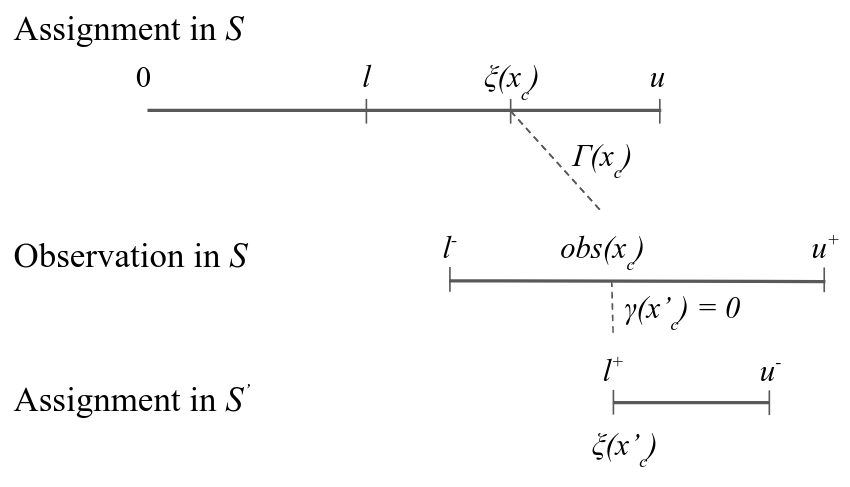
\includegraphics[width=3.5in]{images/viz-eqn-obs-assign.png}
\caption{\label{fig:obs-assign}We visualize the relationship between realized assignments across \(S\) and \(S'\). In this example, each horizontal line is a timeline monotonically increasing from left to right. Dashed lines represent observation delays. We see how an assignment in \(S\), \(\assign(x_{c})\), realized observation delay, \(\Gamma(x_{c})\), and an observation in \(S\), \(\obs(x_{c})\), contribute to an assignment in \(S'\), \(\assign(x'_{c})\).}
\end{figure}

Note that we receive \(\obs(x_{c})\) from Nature, but make the assignment \(\xi(x'_{c})\) in the
dispatchable form of \(S'\). To be clear, while \(\assign(x_{c})\) is an interval, \((\mathbb{R} \cup
\infty) \times (\mathbb{R} \cup \infty)\), \(\assign(x'_{c})\) is in \(\mathbb{R}\). For a fixed
interval, e.g. \(\obs(x_{c}) \in [t, t]\), we sometimes employ an equivalent representation,
\(\assign(x_{c}) = t\).


Additionally, we sometimes apply \(-\) and \(+\) superscripts to \(l\) and \(u\) to denote the earliest and
latest times respectively that an assignment at those bounds could be observed. For instance, the
relationship in Definition \ref{defn:vdc-obs} simplifies to,

\begin{align}
\label{eqn:obs-assign}
\label{eqn:obs-assign}
\obs(x_{c}) &= [l + \gammabar^-(x_{c}), u + \gammabar^+(x_{c})] \\
\obs(x_{c}) &= [l^-(x_{c}), u^+(x_{c})]
\end{align}

Lastly, we need a means to compare observation spaces if we are to transform variable-delay to
fixed-delay STNUs.

\begin{defn}
\textbf{Observation Space Mapping}

Let \(\mu\) be a mapping from an assignment to a situation, \(\mu : \xi \rightarrow \omega\). To say
that \(\mu(x'_{c}) \subseteq \omega_{v}(x_{c})\) means that, for any assignment of \(x'_{c}\) in \(S'\),
there is an equivalent situation in \(S\) for \(x_{c}\).
\end{defn}

For the transitions below, it is a \emph{valid observation space mapping}, if we can show that
\(\mu(x'_{c}) \subseteq \omega_{v}(x_{c})\). If so, it is guaranteed that any assignment in the
observation space of \(x'_{c}\) also has a valid assignment in the observation space of \(x_{c}\).

We now have the necessary vocabulary and notation to step through the transformations from \(S\) to
\(S'\). These lemmas were first presented in \citeprocitem{1}{[1]}, with some refinement by us for the
aforementioned journal article submission.

\begin{defn}
\textbf{Variable-Delay to Fixed-Delay Transformations}

The \emph{variable-delay to fixed-delay transformations} define a set of observation space mappings,
where there are valid observation space mappings for all the contingent constraints in \(S'\) to \(S\).
\end{defn}

Thus, if there is a satisfying \(\mathcal{S}\) for the fixed-delay observation space of \(S'\), it is guaranteed to
simultaneously satisfy any situation in the variable-delay observation space, \(\Omega_{v}\), of \(S\).

\begin{lemma}
\label{lemma:emulating-fixed}
For any contingent event \(x_c \in X_c\) in \(S\), if \(\gammabar^-(x_c) = \gammabar^+(x_c)\), we emulate
\(\gammabar(x_c)\) in \(S'\) using \(\gamma(x'_c) = \gammabar^+(x_c)\).
\end{lemma}

\begin{proof}
We translate an already fixed-bounded observation delay in the form of \(\gammabar(x_{c})\) to the
equivalent fixed-delay function, \(\gamma(x'_{c})\), thus \(\omega_{f}(x'_{c}) = \omega_{v}(x_{c})\).
\end{proof}

\begin{lemma}
\label{lemma:partially-unobservable}
For any contingent event \(x_c \in X_c\), \(\gammabar^+(x_c) = \infty\), we emulate \(\gammabar(x_c)\) in
\(S'\) as \(\gamma(x'_c) = \infty\).
\end{lemma}

\begin{proof}
There are projections where we would not receive information about \(x_{c}\), therefore we have to act
as if we \emph{never} receive an observation of \(x_{c}\). Any \(\mathcal{S}\) that works when we do not
receive information about \(x_{c}\) would also work when do receive an observation if we choose to
ignore the observation.

None of our decisions depend on \(\xi(x'_{c})\), thus no observation space mapping to \(S\) is
necessary.
\end{proof}

\begin{figure}[htbp]
\centering
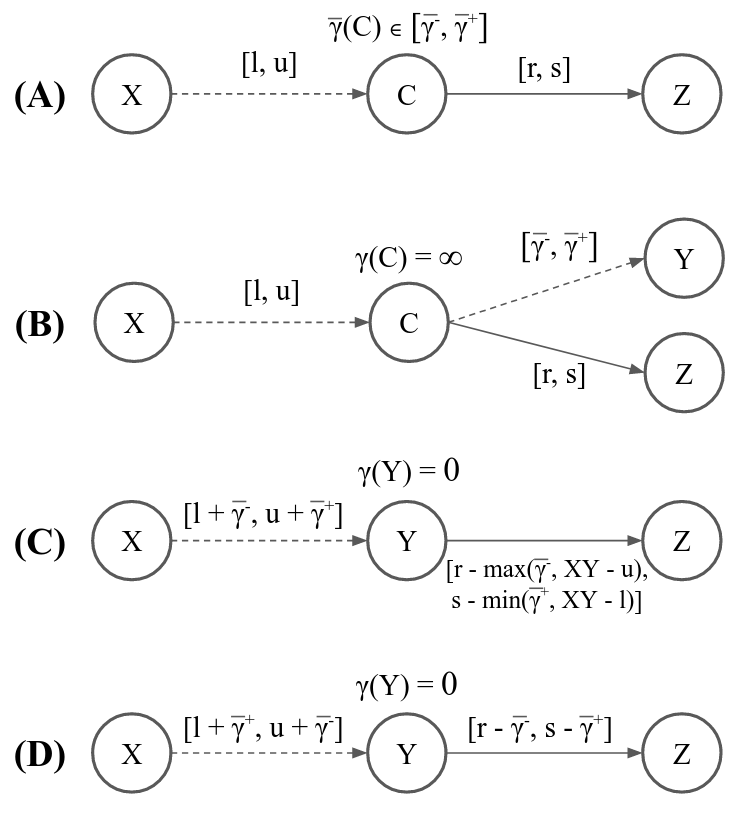
\includegraphics[width=.9\linewidth]{images/lemmas-combined.png}
\caption{\label{fig:lemmas-combined}A visualization of the lemmas used to transform contingent links with variable observation delay and subsequent requirement links.}
\end{figure}

\begin{lemma}
\label{lemma:not-enough-information}
If \(u - l \leq \gammabar^+(x_c) - \gammabar^-(x_c)\), we emulate \(\gammabar(x_c)\) in \(S'\) using
\(\gamma(x'_c) = \infty\).
\end{lemma}

\begin{proof}
We can ignore observations of \(x_{c}\) because they are not guaranteed to narrow where \(\assign(x_c)\)
was assigned in the range \([l, u]\).

Let \(\alpha\) be the range of \(\obs(x_{c})\) when \(\assign(x_{c}) \in [l, l]\). Let \(\beta\) be the
range of \(\obs(x_{c})\) when \(\assign(x_{c}) \in [u, u]\). By Equation \ref{eqn:obs-assign},

\begin{align*}
\alpha &= [l^-(x_{c}), l^+(x_{c})] \\
\beta &= [u^-(x_{c}), u^+(x_{c})]
\end{align*}

We can show that \(u^-(x_{c}) \leq l^+(x_{c})\).

\begin{align*}
u - l &\leq \gammabar^+(x_c) - \gammabar^-(x_{c}) \\
u + \gammabar^-(x_{c}) &\leq l + \gammabar^+(x_{c}) \\
u^-(x_{c}) &\leq l^+(x_{c})
\end{align*}

The lower bound of \(\beta\) is less than the upper bound of \(\alpha\), thus \(\alpha \cap \beta\). An
observation \(\obs(x_{c}) \in [u^-(x_{c}), l^+(x_{c})]\) could be the result of \(\assign(x_{c}) = [l,
l]\), \(\assign(x_{c}) = [u, u]\), or any value \(\assign(x_{c}) \in [l, u]\). Observations provide no
information about the underlying contingent constraint, therefore we ignore \(\obs(x_{c})\).

None of our decisions depend on \(\xi(x'_{c})\), thus no observation space mapping to \(S\) is
necessary.
\end{proof}

\begin{lemma}
\label{lemma:main-tightening}
If \(u - l > \gammabar^+(x_c) - \gammabar^-(x_c)\), we can emulate \(\gammabar(x_c)\) under minimal
information by replacing the bounds of \(x_c\) with \(x'_{c} \in [l^+(x_{c}), u^-(x_{c})]\) and letting
\(\gamma(x'_c) = 0\).
\end{lemma}

\begin{proof}
Under Lemma \ref{lemma:main-tightening}, observations \(\obs(x_{c})\) are guaranteed to narrow the range of
\(\assign(x_{c})\).

We have the same ranges for \(\alpha\) and \(\beta\) as in Lemma \ref{lemma:not-enough-information}, however
we can show that \(u^-(x_{c}) \geq l^+(x_{c})\) instead.

\begin{align*}
u - l &\geq \gammabar^+(x_c) - \gammabar^-(x_{c}) \\
u + \gammabar^-(x_{c}) &\geq l + \gammabar^+(x_{c}) \\
u^-(x_{c}) &\geq l^+(x_{c})
\end{align*}

Thus, receiving an observation is guaranteed to narrow the derived range of \(\assign(x_{c})\). The
transformation tightens the range of \(x'_{c}\) to one where there is maximum ambiguity of the
assignment of \(x_{c}\) while guaranteeing an execution strategy for any assignment of \(x_{c} \in [l,
u]\).
\end{proof}

After applying Lemma \ref{lemma:main-tightening}, despite the limited expected range of assignments in
\(x'_{c}\) in \(S'\) compared to \(x_{c}\) in \(S\), we can show that Lemma \ref{lemma:applied-execution}
guarantees a satisfying schedule for any \(\obs(x_{c}) \in [l^-(x_{c}), u^+(x_{c})]\) using an
\(\mathcal{S}\) that employs \emph{buffering} and \emph{imagining} contingent events.

\begin{defn}
\textbf{Buffering}

\emph{Buffering} a contingent event \(x_{c}\) is an execution strategy where, if \(x_{c}\) is observed
earlier than the lower bound of the observation space \(\obs(x_{c}) < \omega_{f}^-(x'_{c})\), we
assign \(\xi(x'_{c})\) to the lower bound of the observation space, \(\xi(x'_{c}) =
\omega_{f}^-(x'_{c})\).
\end{defn}

\begin{defn}
\textbf{Imagining}

\emph{Imagining} a contingent event \(x_{c}\) is an execution strategy where, if \(x_{c}\) is observed later
than the upper bound of the observation space, \(\obs(x_{c}) > \omega_{f}^+(x'_{c})\), we assign
\(\xi(x'_{c})\) to the upper bound of the observation space, \(\xi(x'_{c}) = \omega_{f}^+(x'_{c})\).
\end{defn}

\begin{lemma}
\label{lemma:buffering-imagining}
If \(S'\) is fixed-delay controllable after applying Lemmas \ref{lemma:main-tightening}, \ref{lemma:execution},
and \ref{lemma:applied-execution} to contingent event \(Y\) with following requirement event \(Z\), there is a
valid \(\mathcal{S}\) for any observation in the observation space of \(S\), \(\omega_{v}(Y) = [a^-(Y),
b^+(Y)]\).
\end{lemma}

\begin{proof}
We first note the observation space of \(S'\) is a subinterval of the original observation space of
\(S\), \(\omega_{f}(Y') \subset \omega_{v}(Y)\), and there are two distinct ranges of observations that
are not in \(\omega_{f}(Y')\).

\begin{align*}
\omega_{f}(Y') &= [a + \gammabar^+(Y), b + \gammabar^-(Y)];~\omega_{v}(Y) = [a + \gammabar^-(Y), b + \gammabar^+(Y)] \\
\omega_{f}(Y') &\not\supset [a + \gammabar^-(Y), a + \gammabar^+(Y))~~(\textit{"Early" observations}) \\
\omega_{f}(Y') &\not\supset (b + \gammabar^+(Y), b + \gammabar^+(Y)]~~(\textit{"Late" observations})
\end{align*}

We address the early observations first. The range of early assignments of \(\xi(Y)\) in \(S\) that we
care about are the ones that could produce an observation \(\obs(Y) \leq a + \gammabar^+(Y)\), which
is \(\xi(Y) = [a, a + (\gammabar^+(Y) - \gammabar^-(Y))]\). We rewrite the range of early assignments
as \(\xi(Y) = a + (\gammabar^+(Y) - \gammabar^-(Y)) - \epsilon\), where \(0 \leq \epsilon \leq
(\gammabar^+(Y) - \gammabar^-(Y))\). By the semantics of \(S\), the range of assignments of \(\xi(Z)\) is
then,

\begin{align*}
\xi(Z) &= [a + (\gammabar^+(Y) - \gammabar^-(Y)) - \epsilon, a + (\gammabar^+(Y) - \gammabar^-(Y)) - \epsilon] + [u, v] \\
\xi(Z) &= [a + u + (\gammabar^+(Y) - \gammabar^-(Y)) - \epsilon, a + v + (\gammabar^+(Y) - \gammabar^-(Y)) - \epsilon]
\end{align*}

The earliest assignment of \(Y'\) in \(S'\) is \(\xi(Y') = a + \gammabar^+(Y)\). By the semantics of \(S'\),
the range of assignments of \(\xi(Z')\) is then,

\begin{align*}
\xi(Z') &= [a + \gammabar^+(Y), a + \gammabar^+(Y)] + [u - \gammabar^-(Y), v - \gammabar^+(Y)] \\
\xi(Z') &= [a + u + (\gammabar^+(Y) - \gammabar^-(Y)), a + v]
\end{align*}

We see that \(\xi(Z') \subseteq \xi(Z)\) for any \(\epsilon\), meaning the execution strategy when
\(\xi(Y') = a + \gammabar^+(Y)\) results in a valid assignment of \(\xi(Z)\) for all early observations
of \(\xi(Y)\). We are safe to buffer early observations to \(\xi(Y') = a + \gammabar^+(Y)\).

We use the same argument for imagining late observations. The range of late assignments of \(\xi(Y)\)
in \(S\) that we care about are the ones that could produce an observation \(\obs(Y) \geq b +
\gammabar^-(Y)\), which is \(\xi(Y) = b - (\gammabar^+(Y) - \gammabar^-(Y)) + \epsilon\). By the
semantics of \(S\), the range of assignments of \(\xi(Z)\) is then,

\begin{align*}
\xi(Z) &= [b - (\gammabar^+(Y) - \gammabar^-(Y)) + \epsilon, b - (\gammabar^+(Y) - \gammabar^-(Y)) + \epsilon] + [u, v] \\
\xi(Z) &= [b + u - (\gammabar^+(Y) - \gammabar^-(Y)) + \epsilon, b + v - (\gammabar^+(Y) - \gammabar^-(Y)) + \epsilon]
\end{align*}

The last assignment of \(Y'\) in \(S'\) is \(\xi(Y') = b + \gammabar^-(Y)\). By the semantics of \(S'\),
the range of assignments of \(\xi(Z')\) is then,

\begin{align*}
\xi(Z') &= [b + \gammabar^-(Y), b + \gammabar^+(Y)] + [u - \gammabar^-(Y), v - \gammabar^+(Y)] \\
\xi(Z') &= [b + u, b + v - (\gammabar^+(Y) - \gammabar^-(Y))]
\end{align*}

We see that \(\xi(Z') \subseteq \xi(Z)\) for any \(\epsilon\), meaning the execution strategy when
\(\xi(Y') = b + \gammabar^-(Y)\) results in a valid assignment of \(\xi(Z)\) for all late observations
of \(\xi(Y)\). In practice, there is no reason to wait until after \(\obs(Y) = b + \gammabar^-(Y)\) to
receive a late observation. As soon as we see the clock has reached \(b + \gammabar^-(Y)\), we are
safe to imagine that \(\obs(Y)\) has been received.
\end{proof}

This concludes the modifications required to transform a contingent event \(x_{c} \in X_{c}\) in \(S\)
to its equivalent \(x'_{c} \in X_{c}\) in \(S'\). What remains is to address the transformation of
requirement links, \(x_{r} \in X_{r}\), in \(S\) such that their transformed equivalents, \(x'_{r} \in
X_{r}\) in \(S'\), express the same execution semantics in \(S'\) as they did in \(S\). We will demonstrate
the correctness of the transformations after Lemma \ref{lemma:applied-execution}.

\begin{lemma}
\label{lemma:execution}
If we have contingent link \(\conedge{X}{C}{}\) with duration \([l, u]\), outgoing requirement link
\(\edge{C}{Z}{}\) with duration \([u, v]\) with an unobservable \(C\), and contingent link
\(\conedge{C}{Y}{}\) with range \([\gammabar^-(x_{c}), \gammabar^+(x_{c})]\), we can emulate the role of
the original requirement link during execution with a new link \(\edge{Y}{Z}{}\) with bounds \([u -
max(\gammabar^-(x_{c}), XY - u), v - min(\gammabar^+(x_{c}), XY - l)]\), where \(XY\) is the true
duration of \(\conedge{X}{Y}{}\).
\end{lemma}

\begin{proof}
See Figure \ref{fig:lemmas-combined}c for reference. From an execution perspective, \(X\) and \(Y\) are
the only events that can give us any information that we can use to reason about when to execute \(Z\)
(since \(C\) is wholly unobservable).

If we execute \(Z\) based on what we learn from \(Y\), then we use our information from \(Y\) to make
inferences about the true durations of \(\conedge{X}{C}{}\) and \(\conedge{C}{Y}{}\) based on
\(\conedge{X}{Y}{}\). We know that the lower-bound of \(\conedge{C}{Y}{}\) is at least \(XY - b\) and that
its upper-bound is at most \(XY - a\). But we also have the a priori bounds on the contingent link
that limit its range to \([\gammabar^-, \gammabar^+]\). Taken together, during execution we can infer
that the true bounds of \(\conedge{C}{Y}{}\) are \([max(\gammabar^-, XY - b), min(\gammabar^+, XY -
a)]\). Since we have bounds only on \(Z\)'s execution in relation to \(C\), we can then infer a
requirement link \(\edge{Y}{Z}{}\) with bounds \([u - max(\gammabar^-, XY - b), v - min(\gammabar^-,
XY - a)]\).

If we try to execute \(Z\) based on information we have about \(X\), we must be robust to any possible
value assigned to \(\conedge{X}{C}{}\). This means that we would be forced to draw a requirement link
\(\edge{X}{Z}{}\) with bounds \([u+b, v+a]\). But we know that \(u - max(\gammabar^-, XY - b) \leq u +
b - XY\) and \(v - min(\gammabar^-, XY - a) \geq v + a - XY\), which means that the bounds we derived
from \(Y\) are at least as expressive as the bounds that we would derive from \(X\).
\end{proof}

Since we have a local execution strategy that depends on the real value of \(XY\), we can try to apply
this strategy to the contingent link that we restricted in Lemma \ref{lemma:main-tightening}, in
order to repair the remaining requirement links.

\begin{lemma}
\label{lemma:applied-execution}
If we have an outgoing requirement link \(\edge{C}{Z}{}\) with duration \([u, v]\), where \(C\) is a
contingent event, we can emulate the role of the original requirement link by replacing its bounds
with \([u - \gammabar^-(x_{c}), v - \gammabar^+(x_{c})]\).
\end{lemma}

\begin{proof}
See Figure \ref{fig:lemmas-combined}d for reference. If we directly apply the transformation from Lemma
\ref{lemma:execution} and Figure \ref{fig:lemmas-combined}c to our original STNU, we introduce complexity
through the need to reason over \(min\) and \(max\) operations in our link bounds. However, from Lemma
\ref{lemma:main-tightening}, we know that in a controllability evaluation context, it is acceptable
for us to simplify the \(\conedge{X}{Y}{}\) link to a stricter range of \([a + \gammabar^+, b +
\gammabar^-]\), instead of \([a + \gammabar^-, b + \gammabar^+]\). This means that for the purpose of
evaluating controllability, we can assume \(a + \gammabar^+ \leq XY \leq b + \gammabar^-\). When we
evaluate the requirement link \(\edge{Y}{Z}{}\), we see \(max(\gammabar^-, XY - b) = \gammabar^-\) and
\(min(\gammabar^+, XY - a) = \gammabar^+\). This gives us bounds of \([u - \gammabar^-, v -
\gammabar^+]\) for the \(\edge{Y}{Z}{}\) requirement link as seen in Figure \ref{fig:lemmas-combined}d.
\end{proof}

Lemma \ref{lemma:applied-execution} handles outgoing requirement edges connected to contingent
events. In addition, we must handle incoming edges.

\begin{corollary}
\label{corollary:reversed}
If we have an incoming requirement link \(\edge{Z}{C}{}\) with duration \([u, v]\), where \(C\) is a
contingent event, we can replace the bounds of the original requirement link with \([u +
\gammabar^+(x_{c}), v + \gammabar^-(x_{c})]\).
\end{corollary}

\begin{proof}
A requirement link \(\edge{Z}{C}{}\) with bounds \([u, v]\) can be immediately rewritten as its reverse
\(\edge{C}{Z}{}\) with bounds \([-v, -u]\). After reversing the edge, we can apply Lemma
\ref{lemma:applied-execution} to get \(\edge{Y}{Z}{}\) with bounds \([-v - \gammabar^-, -u -
\gammabar^+]\), which we can reverse again to get \(\edge{Z}{Y}{}\) with bounds \([u + \gammabar^+, v +
\gammabar^-]\).
\end{proof}

We can examine a concrete example of Lemmas \ref{lemma:main-tightening}, \ref{lemma:execution}, and
\ref{lemma:applied-execution} to show equivalence in the transformation from Figure \ref{fig:lemmas-combined}a
to \ref{fig:lemmas-combined}d. We start by building an example of \ref{fig:lemmas-combined}a. Let
\(\conedge{X}{C}{[2, 5]}\) with \(\gammabar(C) \in [1, 2]\) and \(\edge{C}{Z}{[11, 20]}\). If we learn of
event \(C\) at time 4, then one possibility is that the realized duration of \(C\) could have been 2
with an observation delay of 2. In this case, event \(Z\) must be executed in \([13, 22]\). However, if
the realized duration of \(C\) were 3 with an observation delay of 1, then \(Z\) would fall in \([14,
23]\). Given we cannot distinguish between the possibilities, we take the intersection of the
intervals, yielding \(Z \in [14, 22]\). Likewise, if we learn of \(C\) at time 6, then \(C\) could have
been realized at time 5 with an observation delay of 1 or it could have been realized at time 4 with
an observation delay of 2. In the first case, \(Z\) must then fall in \([16, 25]\), while in the second,
\(Z\) would fall in \([15, 24]\). The intersection yields \([16, 24]\).

By the semantics represented in Figure \ref{fig:lemmas-combined}d, we can build an equivalent network with
\(\gamma(Y) = 0\) by setting \(\conedge{X}{Y}{[4, 6]}\) and \(\edge{Y}{Z}{[10, 18]}\). If \(Y\) is observed
at time 4, \(Z\) must be executed in \([14, 22]\). If \(Y\) is observed at time 6, \(Z\) then must be
executed in \([16, 24]\). The execution semantics for both cases match the equivalent networks from
\ref{fig:lemmas-combined}a described above.

\section{Discussion}
\label{sec:orgc37ea10}

We have demonstrated a modeling formalism to describe temporal networks with uncertain observation
delay, along with a sound and complete procedure for checking controllability of said temporal
networks. VDC is sound because if it finds that \(S'\) has a valid execution strategy, then it must
also be the case that \(S\) has an execution strategy. VDC is complete because if it finds that \(S'\)
is not controllable, then there exists a projection of \(S\) that is uncontrollable, thus \(S\) is not
variable-delay controllable.

\section{Experimental Analysis}
\label{sec:orgcef7059}
\label{sec:vdc-experimental}

In this section, we provide empirical evaluations of our variable-delay controllability checking
algorithms, showing that variable-delay controllability gives us a level of modeling expressiveness
that cannot be captured by approximations that use delay controllability alone. We do so by
constructing examples of variable-delay STNUs for realistic multi-agent coordination scenarios that
are taken from the domain of planetary exploration, inspired by the real decision-making processes
during Apollo EVAs and modern day EVA operations research. First, we briefly describe the
operational environment, relevant actors, and decisions in EVAs. We then provide a selection of
STNUs that reflect the activities and temporal constraints of planetary exploration. Using these
building blocks, we make a case for the expressivity of VDC in modeling uncertain communication,
then generate larger STNUs to demonstrate the soundness of variable-delay controllability
checking.\footnote{The implementation of the experiments herein can be found at
\href{https://gitlab.com/mit-mers/delay-stnu-benchmarks}{[https://gitlab.com/mit-mers/delay-stnu-benchmarks}].}

\begin{figure}[htbp]
\centering
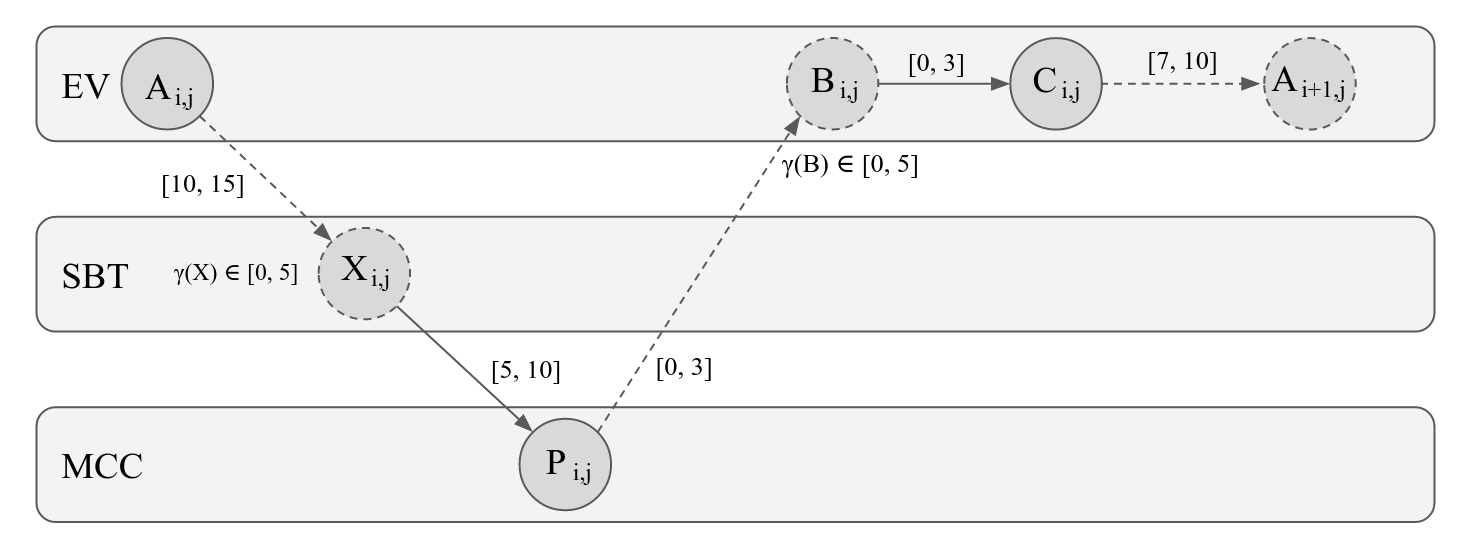
\includegraphics[width=1\textwidth]{images/eva-stnu.png}
\caption{\label{fig:sbt-stnu}An STNU representing an EVA sampling task. The episode durations are representative of the bounds used in simulation. The depiction of this STNU with variable-delay is presented with rows representing actors to clarify the context of each event.}
\end{figure}

Now, we present a sample collection communication scenario in Figure \ref{fig:sbt-stnu} that is
representative of the types of activities performed during exploration and requires uncertain
communication delay to faithfully model.

At a high level, in this activity a crew of \(i\) astronauts perform \(j\) activities of scanning
potential samples and receiving feedback from the science team as to whether they should store or
discard those sample. Scanning requires liberating, that is chipping away, a piece of rock from an
outcrop, \(A_{i,j}\), and performing a scan of the newly exposed surface with a handheld spectrometer.
Spectroscopy data is eventually received at \(X_{i,j}\); we model this duration of this process with
the contingent link \(\conedge{A_{i,j}}{X_{i,j}}{}\) where \(X_{i,j}\) is uncontrollable because the
time to liberate and scan is a function of the environment (eg. how hard the sample is to access),
not the crew. The processing completion time of the handheld spectrometer is highly variable, and as
such we have \(\gammabar({X_{i,j}})\) represent a variable delay in receiving the results of the scan.
Interestingly, note that the general time of \(A_{i,j}\) will be known immediately through the use of
audio and video communications - the variability of \(X_{i,j}\) refers to the delay of receiving the
spectroscopy data itself.

During a narrow window of opportunity between the receipt of the sample information and a deadline
imposed by Mission Control, \(P_{i,j}\), the science team must confer and decide on a sample
collection priority list to send to Mission Control, \(\edge{X_{i,j}}{P_{i,j}}{}\). Even once Mission
Control has a sample priority list in hand, \(P_{i,j}\), due to health and safety concerns, they may
prioritize other messages before they send the science team's sampling priority decision to the
crew. As such, the message passing process, \(\conedge{P_{i,j}}{B_{i,j}}{}\), is modeled as
uncontrolled with a variable communication delay. Once the crew receives the priority list, \(B\),
they then stow the requested amount of samples at \(C_{i,j}\). Then the astronaut traverses to the
next location and the procedure repeats anew. We use \(\conedge{C_{i,j}}{A_{i,j+1}}{}\) to model the
time needed to traverse to the site of the next activity. We apply a requirement link with a
lower-bound of 0 and an upper bound of the limiting consumable from the overall start of each STNU
to its overall end after each astronaut has completed all activities.

With realistic STNUs in hand, we can now evaluate the performance of our variable-delay
formulations. For the simulations presented in subsequent sections, we generated STNUs that follow
the form of Figure \ref{fig:sbt-stnu} with randomized bounds on the links and delay functions, as will be
described below.

\begin{table*}[t]
\centering
\begin{tabular}{ |>{\centering\arraybackslash} m{4.4cm}||>{\centering\arraybackslash} m{4.5cm}|>{\centering\arraybackslash} m{5.0cm}|  }
 \hline
 & Variable-delay controllable & Variable-delay uncontrollable\\
 \hline
 \hline
 Min-fixed controllable & 222 & 619\\
 \hline
 Min-fixed uncontrollable & 0 & 159\\
 \hline
 \hline
 Mean-fixed controllable & 222 & 583\\
 \hline
 Mean-fixed uncontrollable & 0 & 195\\
 \hline
 \hline
 Max-fixed controllable & 222 & 355\\
 \hline
 Max-fixed uncontrollable & 0 & 423\\
 \hline
\end{tabular}
\caption{Variable-delay vs. minimum, mean, and maximum fixed-delay controllability results with the parallel installation STNU from Figure \ref{fig:dish-stnu}.}
\label{table:comparison}
\end{table*}

We now will evaluate the comparative quality of variable-delay formulations against fixed-delay
approximations by using the repeater installation scenario seen in Figure \ref{fig:dish-stnu}. We
generate STNUs with four astronauts each performing five installations. We set the lower bounds of
\(\conedge{A_{i,j}}{B_{i,j}}{}\) to 0 and choose the upper bounds from a uniform distribution of
integers between 0 and 20, \(\mathcal{U}_{[0, 20]}\). There is no delay function for \(B_{i,j}\).
Likewise, for \(\edge{B_{i,j}}{C_{i,j}}{}\), we set the lower bounds to 0 and choose an integer upper
bound in \(\mathcal{U}_{[0, 15]}\). \(\conedge{C_{i,j}}{D_{i,j}}{}\) has a lower bound of 0 and an upper
bound integer chosen in \(\mathcal{U}_{[0, 20]}\). The variable-delay function \(\gamma(D_{i,j})\) has a
lower bound of 0 and upper-bound chosen from the exponential distribution \(f(t) = \lambda
e^{-\lambda t}\) with \(\lambda = 3\). \(\conedge{D_{i,j}}{A_{i,j+1}}{}\) takes a lower bound integer,
\(a\), from \(\mathcal{U}_{[10, 20]}\) and its upper bound in \(a + \mathcal{U}_{[4, 10]}\). Lastly, we
pick a random limiting consumable as the multiple of the number of activities and an integer from
\(\mathcal{U}_{[50, 60]}\).

We employ three different strategies for each \(\gamma(x_c)\) in \(S\) for our fixed-delay
approximations: \(\gamma(x_c) = \gammabar^-(x_c)\), \(\gamma(x_c) = \frac{\gammabar^- +
\gammabar^+}{2}\), and \(\gamma(x_c) = \gammabar^+(x_c)\). For each strategy, we know that whenever the
original STNU is variable-delay controllable with respect to \(\gammabar\), it is also fixed-delay
controllable with respect to \(\gamma\). Each choice of \(\gamma\) represents a potential realization of
the delays offered by \(\gammabar\), and the fixed-delay approximation has the added benefit of
eliminating uncertainty in observation.

We generate 1000 different STNUs and compare the variable-delay controllability results to the
different fixed-delay controllability approaches (Table \ref{table:comparison}). Note that our randomly
generated variables, notably the choice of \(\gamma(C_{i,j})\) and the width of the following
\(\edge{C_{i,j}}{D_{i,j}}{}\) link, were selected such that the STNUs generated could be
variable-delay, fixed-delay, dynamic, or strong controllable, or uncontrollable. The instances that
are of greatest interest are those where the STNU is not variable-delay controllable but the
fixed-delay approximations determine it to be controllable.

This false positive rate of the minimum fixed-delay controllability approximation is quite high at
80.0\%. The mean and maximum fixed-delay approximations have more reasonable false positive rates at
74.9\% and 45.6\% respectively. Since all approximations yield the correct answer when the original
STNU is variable-delay controllable, it follows that the maximum fixed-delay approximation has the
lowest false positive rate, as it is the most demanding of the three.

We note that these results are dependent on the width of the variable-delay ranges found in the
network. We can increase the likelihood that a delay takes longer by increasing the choice of
\(\lambda\) in our exponential delay function. When we vary our delay function using \(\lambda = 4.5,
6, 7.5\), and \(9\), the false positives of the max-delay approximation are 27.9\% 12.9\%, 7.0\%, and
3.1\%, respectively.

In addition to simulating the network using fixed-delays, we also consider the effect of combining
the two sources of uncertainty, the duration of the action and the delay in observation, into one
new source of uncertainty. Unlike the fixed-delay approximations, we know that if a network under
this transformation is controllable, then so too is the original network, as this approach discards
any existing knowledge about the difference in uncertainties between the original event and the
observation of that event.

\begin{table*}[t]
\centering
\begin{tabular}{ |>{\centering\arraybackslash} m{4.4cm}||>{\centering\arraybackslash} m{4.5cm}|>{\centering\arraybackslash} m{5.0cm}|  }
 \hline
 & Variable-delay controllable & Variable-delay uncontrollable\\
 \hline
 \hline
 Elongated controllable & 36 & 0\\
 \hline
 Elongated uncontrollable & 186 & 778\\
 \hline

\end{tabular}
\caption{Variable-delay controllability vs. the controllability of a network that elongates its contingent links to account for observational uncertainty when using an exponential delay function with $\lambda = 3$.}
\label{table:comparison-elongated}
\end{table*}

As seen in Table \ref{table:comparison-elongated}, this approach yields no false positives, but still
presents a modestly high false negative rate of 19.3\%. An appropriate approximation strategy can be
adopted to prevent either false positives or false negatives; however, such a wide disparity in
results strongly reinforces the value of modeling observational uncertainty directly.

\chapter{Dynamic Scheduling with Delayed Event Monitoring}
\label{sec:org052d259}
\label{ch:delay-scheduling}

Now that we have shown there exists a valid execution strategy for variable-delay controllable
STNUs, we contribute a novel scheduling and dispatching architecture for online, dynamic execution.
In this Chapter, our aim is to describe the single-agent form of a new instantiation of Kirk, \emph{Delay
Kirk}, that can reason over uncertain observation delay to decide when to execute requirement
events. There are two main components to Delay Kirk: (1) a \emph{delay scheduler}, and (2) a \emph{delay
dispatcher}. As will be shown in Section \ref{sec:delay-scheduling}, scheduling variable-delay
controllable STNUs is an extension to existing dynamic scheduling algorithms with modifications for
the execution strategy shown to be sound and complete in Chapter \ref{ch:modeling-tn}.

Additionally, to the best of our knowledge, scheduling fixed-delay STNUs has not been presented in
the literature. Fixed-delay scheduling is required for addressing (1). As such, we contribute a
fixed-delay scheduler in Section \ref{sec:delay-scheduling}. The execution strategy from Chapter
\ref{ch:modeling-tn} will be shown to be a small extension to the fixed-delay scheduler. As to (2), to the
best of our knowledge, there are no other formalized dispatching algorithms in the literature. In
the development of Delay Kirk, we found it to be extremely useful to formalize dispatching as part
of creating a clear interface boundary between scheduling and dispatching. The dispatching
algorithms we put forth in Section \ref{sec:dynamic-dispatching} represent novel contributions to temporal
reasoning.

This Chapter makes additional contributions to scheduling and dispatching. Safely executing events
on real hardware requires modifications to generating decisions in dynamic scheduling. We include
said modifications, with confluent interfaces in dynamic dispatching, to suit our intended use cases
for Delay Kirk.

In Section \ref{sec:optimistic-rescheduling}, we extend our approach to scheduling variable-delay STNUs by
introducing an optional procedure that addresses a shortcoming in the semantics of scheduling a
variable-delay STNU. The shortcoming takes the form of potentially unnecessary wait times that are
added after receiving contingent event assignments, extending the makespan of procedures. We present
a generate-and-test algorithm to partially mitigate said shortcomings.

Finally, Section \ref{sec:scheduling-experimental} provides a series of benchmarks of the scheduling and
dispatching algorithms described in this Chapter.

\section{Dynamic Scheduling through Real-Time Execution Decisions}
\label{sec:org9730cf7}
\label{sec:dynamic-scheduling}

We first provide a necessary overview of dynamic scheduling of vanilla STNUs, which we will extend
for STNUs with observation delay in Section \ref{sec:delay-scheduling}.

An STNU, \(S\), that exhibits dynamic controllability can be \emph{scheduled} dynamically (or \emph{online}). At
a high-level, dynamic scheduling is the process of mapping the history of event assignments to the
execution time of future free events. We will build off of the scheduling work by Hunsberger
\citeprocitem{36}{[36]}, \citeprocitem{38}{[38]}, which describes an \(O(N^{3})\) online procedure, FAST-EX, for
dynamic scheduling of STNUs. We chose FAST-EX because, to the best of our knowledge, this is the
fastest dynamic scheduling algorithm in the literature today. At its core is the notion of
\emph{Real-Time Execution Decisions} (RTEDs), which map a timepoint to a set of requirement events to be
executed and are generated based on \emph{partial schedules} of STNUs being executed. \texttt{WAIT} decisions
may also be produced, reflecting the need to wait for the assignment of a contingent event before
continuing. RTED-based scheduling applies a dynamic programming paradigm in three steps:

\begin{enumerate}
\item creating a dispatchable form of temporal constraints offline in the form of a distance graph,
\item updating the dispatchable form as the partial schedule is updated online through event
assignments, and
\item querying the dispatchable form online to quickly find the next RTED \citeprocitem{39}{[39]}.
\end{enumerate}

The dispatchable form employed by FAST-EX is the \emph{AllMax} distance graph, which is produced by the
Morris \(O(N^{4})\) DC-checking procedure \citeprocitem{27}{[27]}.

\begin{defn}
\textbf{AllMax Distance Graph} \citeprocitem{26}{[26]}

The \emph{AllMax} distance graph is a distance graph exclusively consisting of unlabeled and upper-case
edges.
\end{defn}

The key idea of FAST-EX is maintaining accurate distances from an artificial zero point, \(Z\), of the
distance graph to all events. At the outset of execution, all events from \(S\) are present as nodes
in \emph{AllMax}. As events are assigned, \emph{AllMax} performs update steps using Dijkstra Single
Source/Sink Shortest Path (SSSP) to maintain distances to unexecuted events, while also collapsing
executed events to \(Z\). We include pseudo-code of the real-time update step in Figure
\ref{alg:fast-ex-update}.

\begin{algorithm}
\SetAlgoLined
\SetKwFunction{Return}{return}
\SetKwInput{Input}{Input}
\SetKwInput{Output}{Output}
\SetKwInput{Algorithm}{\textsc{FAST-EX Update}}
\SetKwInput{Initialize}{Initialization}
\SetKwIF{If}{ElseIf}{Else}{if}{then}{else if}{else}{endif}
\Indm
\Input{Time $t$; Set of newly executed events $\texttt{Exec} \subseteq X_{e} \cup X_{r}$; AllMax Graph $G$; Distance matrix $D$, where $D(A, B)$ is the distance from $A$ to $B$}
\Output{Updated $D$}
\Indp
\Algorithm{}
\Indp
\For{each contingent event $C \in \texttt{Exec}$} {
    Remove each upper-case edge, $\edge{Y}{A}{C:-w}$, labled by $C$\;
    Replace each edge from $Y$ to $Z$ with the strongest replacement edge\;
}
\For{each event $E \in \texttt{Exec}$} {
    Add lower-bound edge $\edge{E}{Z}{-t}$\;
}
For each event $X$, update $D(X, Z)$ using Dijkstra Single-Sink Shortest Paths\;
\For{each event $E \in \texttt{Exec}$} {
    Add upper-bound edge $\edge{Z}{E}{t}$\;
}
For each event $X$, update $D(Z, X)$ using Dijkstra Single-Source Shortest Paths\;
\caption{Algorithm for updating distances for all events in relation to $Z$ upon the execution of an event. Adapated from \citeprocitem{3}{[3]}, Fig. 19.}
\label{alg:fast-ex-update}
\end{algorithm}

With an up-to-date distance graph in hand, we can perform an online query for the current RTED.

\begin{defn}
\textbf{Real-Time Execution Decisions} \citeprocitem{39}{[39]}

A \emph{Real-Time Execution Decision} is a two-tuple \(\langle t, \chi \rangle\), where:
\begin{itemize}
\item \(t\) is a time with domain \(\mathbb{R}\),
\item \(\chi\) is a set of \(x_{r} \in X_{r}\) to be executed at time \(t\)
\end{itemize}
\end{defn}

Let \(U_{x}\) be the set of unexecuted free timepoints. If \(U_{x}\) is empty, then the RTED is to
\texttt{WAIT}. Otherwise, we find the lower bound of the earliest executable time point and the set of
executable events associated with it.

\begin{align}
\label{eqn:rted1}
t &= \min\{-D(X, Z)~|~X \in U_{x}\} \\
\label{eqn:rted-chi}
\chi &= \{X \in U_{x}~|~-D(X, Z) = t\}
\end{align}

We cannot execute events in the past. Let \texttt{now} be the current time, i.e. the last timepoint
captured in the event assignments. It is possible that \(t \leq \texttt{now}\), in which case we must
reassign \(t\) to guarantee that \(t > \texttt{now}\). To do so, we update \(t\) as follows, where \(t^+\)
is earliest upper bound of the executable timepoints,

\begin{align}
\label{eqn:rted2}
t^+ &= \min\{D(Z, X)~|~X \in U_{x}\} \\
\label{eqn:rted-t}
t &= \cfrac{\texttt{now} + t^+}{2}
\end{align}

So long as \(t^+ > \texttt{now}\), we know that the reassignment of \(t\) ensures \(t > \texttt{now}\).

\section{Delay Scheduling as an Extension to Dynamic Scheduling}
\label{sec:orgee95dee}
\label{sec:delay-scheduling}

\begin{figure}[htbp]
\centering
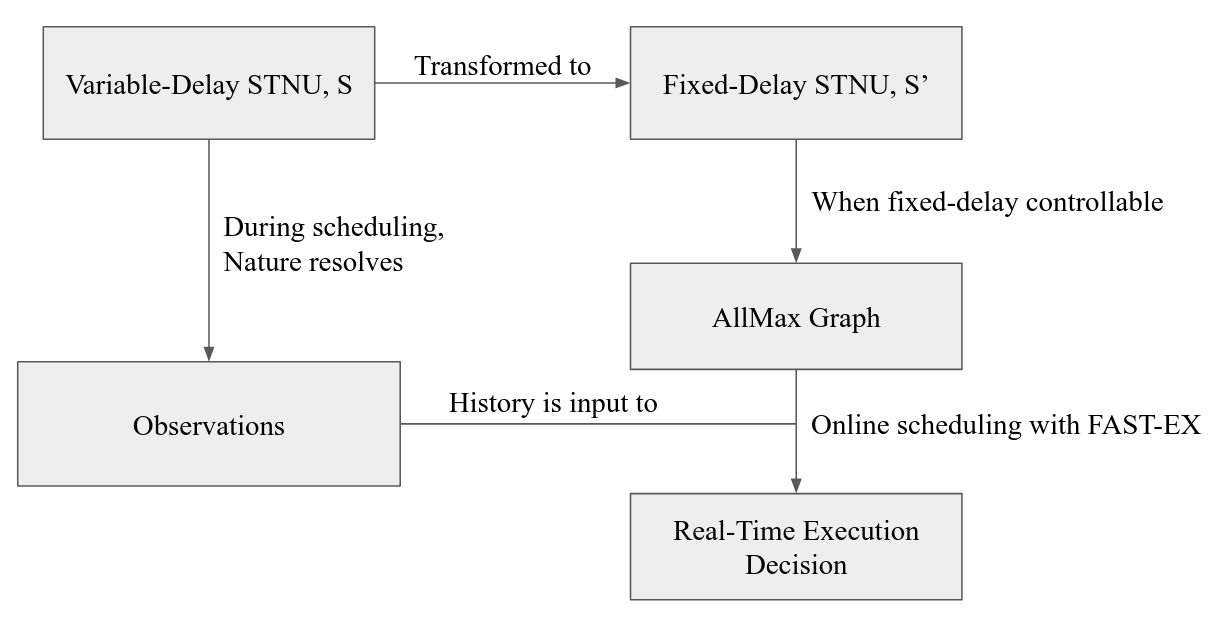
\includegraphics[width=0.8\textwidth]{images/flow-chart.png}
\caption{\label{fig:flow-chart}A high-level flow chart showing how we use variable-delay STNUs to generate scheduling decisions. The boxes represent the data structures involved in scheduling, while the arrows are the processes that are followed to eventually produce RTEDs.}
\end{figure}

Figure \ref{fig:flow-chart} presents a high-level overview of the information flow in the scheduling
process.

In order to schedule a variable-delay STNU, the core problem we must address is that, to date, there
is no means to directly create a corresponding dispatchable form that accounts for uncertain
assignments resulting from variable observation delay. We encountered this same problem when
describing the process of checking VDC in Section \ref{sec:vdc}. We overcame this limitation by first
transforming the variable-delay STNU to a fixed-delay STNU before checking FDC. A similar strategy
will be followed for scheduling in that we will transform the variable-delay to a fixed-delay STNU,
then dispatch events using the dispatchable form of the fixed-delay STNU instead. However, doing so
creates a second problem. While we will be performing FAST-EX against the fixed-delay STNU, the
contingent event observations we receive will adhere to the constraints and variable-delay function
of the variable-delay STNU. Hence, we must modify our real-time update and RTED generation
algorithms to account for early and late contingent event observations.

We start by providing an explanation of fixed-delay scheduling, before expanding it to address the
execution strategies of variable-delay scheduling.

\subsection{Fixed-Delay Scheduling}
\label{sec:orga83b318}

We first establish the algebra of receiving observations.

\begin{lemma}
\label{lemma:information-fixes-bounds}
For any contingent event, \(x_{c} \in S\) or \(x'_{c} \in S'\), observing \(x_{c}\) at time \(t \in
[l^-(x_{c}), u^+(x_{c})]\) fixes the observation to \(\obs(x_{c}) = [t, t]\).
\end{lemma}
\begin{proof}

Prior to execution, an observation of \(x_{c}\) may fall anywhere within the set-bounded interval from
the earliest possible observation at \(l^-(x_{c})\) to the last possible observation at \(u^+(x_{c})\).
Receiving an observation \(\obs(x_{c}) = t\) during execution eliminates all possible observations
outside the interval \([t, t]\).
\end{proof}

\begin{lemma}
\label{equal-is-fixed-bounds}
For any temporal constraint, \(x\), with bounds \(x \in [l, u]\) for some \(l\) and \(u\), and timepoint \(t
\in [l, u]\), if information reduces the bounds of \(x\) to \(x \in [t, t]\), we may assert \(x = t\).
\end{lemma}

\begin{proof}

When the bounds of an interval, \(x \in [l, u]\) are fixed such that \(t = l = u\), we can assert that
\(x\) must have resolved to \(t\).
\end{proof}

\begin{lemma}
\label{lemma:subtract-gamma}
For any contingent event \(x'_{c} \in X_{c}\) in fixed-delay controllable \(S'\), if \(\gamma(x'_{c}) \in
\mathbb{R}\), we assign \(\assign(x'_{c}) = \obs(x_{c}) - \gamma(x'_{c})\) in the dispatchable form of
\(S'\).
\end{lemma}

\begin{proof}
The central challenge of checking fixed-delay controllability is determining that an execution
strategy exists that allows an agent to wait an additional \(\gamma(x'_{c})\) time units after a
contingent event has been assigned to learn its outcome. Importantly, the \(\gamma\) function is not
used to modify the edges of the labeled distance graph, which are derived from the constraints \(r
\in R_{e} \cup R_{c}\) in \(S'\).

As \(\gamma(x'_{c})\) resolves to a known and finite value, we can derive the true value of
\(\assign(x'_{c})\) to be assigned in the labeled distance graph. Contingent event assignments are
recorded in the labeled distance graph as follows, where \(\obs(x_{c})\) is the resolved observation,

\begin{align}\assign(x'_c) = \obs(x_c) - \gamma(x'_c) \label{eqn:fixed-recording}
\end{align}
\end{proof}

The FAST-EX real-time update algorithm, Algorithm \ref{alg:fast-ex-update}, then becomes Algorithm
\ref{alg:fast-ex-fixed-obs}.

\begin{algorithm}
\SetAlgoLined
\SetKwFunction{Return}{return}
\SetKwInput{Input}{Input}
\SetKwInput{Output}{Output}
\SetKwInput{Algorithm}{\textsc{FAST-EX Update with Fixed Observation Delay}}
\SetKwInput{Initialize}{Initialization}
\SetKwIF{If}{ElseIf}{Else}{if}{then}{else if}{else}{endif}
\Indm
\Input{Time $t$; Set of newly observed events $\texttt{Exec} \subseteq X_{e} \cup X_{r}$; AllMax Graph $G$; Distance matrix $D$, where $D(A, B)$ is the distance from $A$ to $B$; Fixed-delay function $\gamma$;}
\Output{Updated $D$}
\Indp
\Algorithm{}
\Indp
\For{each contingent event $C \in \texttt{Exec}$} {
    $\assign(C) \leftarrow \obs(C) - \gamma(C)$\;
    Remove each upper-case edge, $\edge{Y}{A}{C:-w}$, labled by $C$\;
    Replace each edge from $Y$ to $Z$ with the strongest replacement edge\;
}
\For{each event $E \in \texttt{Exec}$} {
    Add lower-bound edge $\edge{E}{Z}{-t}$\;
}
For each event $X$, update $D(X, Z)$ using Dijkstra Single-Sink Shortest Paths\;
\For{each event $E \in \texttt{Exec}$} {
    Add upper-bound edge $\edge{Z}{E}{t}$\;
}
For each event $X$, update $D(Z, X)$ using Dijkstra Single-Source Shortest Paths\;
\caption{Algorithm for updating distances for all events in relation to $Z$ upon the execution or observation of an event.}
\label{alg:fast-ex-fixed-obs}
\end{algorithm}

No other modifications to FAST-EX are required to schedule a fixed-delay STNU.

\subsection{Variable-Delay Scheduling}
\label{sec:org44c55af}

Our execution strategy must address each of the following special categories of contingent event
observations:

\begin{enumerate}
\item contingent events with infinite observation delay,
\item contingent events that are observed outside \([l^+(x_{c}), u^-(x_{c})]\) in \(S'\).
\end{enumerate}

The first category is a requirement for dispatching the fixed-delay equivalent of a variable-delay
STNU. If the constraints of a problem domain are modeled directly in a fixed-delay STNU and the
modeler gives a contingent event, \(x_{c}\), infinite delay, e.g. \(\gamma(x_{c}) = \infty\), the event
will never be observed and thus a fixed-delay scheduler has no need for an execution strategy in the
event that \(x_{c}\) is observed. However, by Lemmas \ref{lemma:partially-unobservable} and
\ref{lemma:not-enough-information} there are some contingent events with potentially finite observation
delay in \(S\) that are transformed to infinite observation delay in \(S'\), making it possible that the
scheduler receives observations of them.

\begin{lemma}
\label{lemma:ignore-inf-delay}
For any contingent event \(x'_{c} \in X_{c}\) in fixed-delay controllable \(S'\), if \(\gamma(x'_{c}) =
\infty\), we mark the event executed but do not assign \(\assign(x'_{c})\) in the dispatchable form of
\(S'\).
\end{lemma}

\begin{proof}
If we are scheduling a fixed-delay STNU, \(S'\), that is already known to be fixed-delay controllable,
an execution strategy must exist that is independent of the assignment of \(\assign(x'_{c})\) when
\(\gamma(x'_{c}) = 0\). We are not required to record \(\assign(x'_{c})\) when \(\gamma(x'_{c}) = \infty\)
to guarantee controllability and may safely ignore it.

We mark the event executed to prevent it from appearing in future RTEDs.
\end{proof}

\begin{figure}[htbp]
\centering
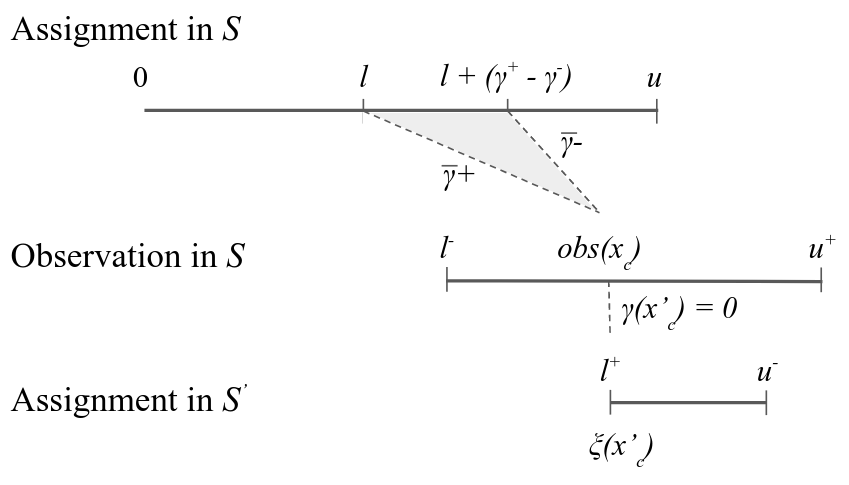
\includegraphics[width=3in]{images/viz-l-plus.png}
\caption{\label{fig:observations}Here, we show how the combination of \(\assign(x_{c})\) and \(\gammabar(x_{c})\) lead to an assignment of \(\assign(x'_{c})\) in \(S'\). We see the range \(\alpha \in [l, l + \gammabar^+(x_{c}) - \gammabar^-(x_{c})\) representing the earliest and latest assignments of \(\assign(x_{c})\) that could result in \(\obs(x_{c}) \in \assign(x'_{c}) \in [l^+(x_{c})\), l\^{}+(x\textsubscript{c})]\$. The grey region represents the range of possible observation delays, \(\gammabar(x_{c})\), supporting \(\assign(x'_{c}) \in [l^+(x_{c}), l^+(x_{c})]\).}
\end{figure}

The second category refers to the need for buffering and imagining events as a result of Lemma
\ref{lemma:main-tightening} using the execution strategy proven to be valid in Lemma
\ref{lemma:buffering-imagining}. There are three regimes of contingent event observations to address.

\begin{enumerate}
\item \(\obs(x_{c})  \in [l^-(x_{c}), l^+(x_{c}))\), ie. strictly earlier than the range
of \(\assign(x'_{c})\),
\item \(\obs(x_{c}) \in [l^+(x_{c}), u^-(x_{c})]\), ie. the range equivalent to \(x'_{c}\), and
\item \(\obs(x_{c}) \in(u^-(x_{c}), u^+(x_{c})]\), ie. strictly later than the range of
\(\assign(x'_{c})\).
\end{enumerate}

Note that we omit the \(-\gamma(x'_{c})\) term from Equation \ref{eqn:fixed-recording} in this analysis due
to the fact that \(\gamma(x'_{c}) = 0\) after applying Lemma \ref{lemma:main-tightening}.

Our execution strategy is to then make the following assignments during the FAST-EX real-time
update.

\begin{equation}
\assign(x'_c) = \begin{cases}
$l^+(x_{c})$  & \text{if } $\obs(x_{c}) \in [l^-(x_{c}), l^+(x_{c}))$ \textit{(buffering)} \\
$\obs(x_{c})$ & \text{if } $\obs(x_{c}) \in [l^+(x_{c}), u^-(x_{c})]$ \\
$u^-(x_{c})$  & \text{if } $\obs(x_{c}) \in (u^-(x_{c}), u^+(x_{c})]$ \textit{(imagining)}
\end{cases}
\end{equation}

In the last case, late observations are assigned to an earlier time. During execution, time is
always increasing. There is no need to wait to make an observation after \(u^-(x_{c})\). Instead, we
modify RTED generation, namely Equation \ref{eqn:rted1}, such that we dispatch \(x'_{c}\) at \(u^-(x_{c})\) if
it is not been observed before \(u^-(x_{c})\). Let \(U_{c}\) be the set of unobserved contingent
timepoints.

\begin{align}
\label{rted-with-ctg}
t_{x} &= \min\{-D(X, Z)~|~X \in U_{x}\} \\
t_{c} &= \min\{D(Z, X)~|~X \in U_{c}\} \\
t &= \min\{t_{x}, t_{c}\} \\
\chi_{x} &= \{X \in U_{x}~|~-D(X, Z) = t\} \\
\chi_{c} &= \{X \in U_{c}~|~D(Z, X) = t\} \\
\chi &= \chi_{x} \cup \chi_{c}
\end{align}

We see that RTEDs may now include unobserved (or unexecuted) contingent timepoints at their upper
bounds. Note that there is no need to distinguish between contingent events that are the result of
tightening during the fixed-delay transformation by applying Lemma \ref{lemma:main-tightening} and others.
We assume that the contingent constraints of the variable-delay STNU accurately reflect Nature. The
latest any other contingent event should be observed is their upper bound in \(S'\) and thus should
never be in the set of events, \(\chi\), of an executed RTED.

We have defined variable-delay execution strategies for when contingent events have infinite delay
and tightened constraints. The remaining category of contingent events is when a contingent event
has a finite, non-zero \(\gamma(x'_{c})\) in \(S'\). If that is the case, \(x'_{c}\) must have had fixed
observation delay in \(S\), Lemma \ref{lemma:emulating-fixed}, and can be scheduled normally after backing
out the observation delay with Equation \ref{eqn:fixed-recording}.

We have addressed the key issue of reconciling observations from \(S\) with the dispatchable form from
\(S'\). We now present a dispatcher and wrapper algorithms on top of FAST-EX that combine to add
robustness for variable observation delay.

\section{Dynamic Dispatching of STNUs with Observation Delay}
\label{sec:orge21d1c5}
\label{sec:delay-scheduler}

The terms ``scheduling'' and ``dispatching'' are often used interchangeably in temporal reasoning
literature. However, we distinguish the goals of a scheduler, as described above, and a dispatcher.

\begin{itemize}
\item \textbf{Scheduling} Generating RTEDs based on a partial schedule
\item \textbf{Dispatching} Reasoning over a clock and RTEDs to guarantee requirement events are safely (w.r.t.
controllability) executed
\end{itemize}

Thus our aim is to

We present an overview of the scheduling algorithm below with explanations following.

While we made a careful distinction between \(x_{c}\) and \(x'_{c}\) in our discussion of scheduling, in
our implementation it was important to be able to easily replace one with another when looking up
values in hash-tables and lists. For instance, to implement Equation \ref{eqn:fixed-recording}, we receive
\(x_{c}\) but key the fixed-delay function on \(x'_{c}\). Rather than adding an additional translation
layer, we give each temporal event in \(S\) a unique name, all of which get copied to their equivalent
events in \(S'\). Hash-tables are keyed on event names, vastly simplifying lookups in the AllMax
graph, delay function, and elsewhere.

\subsection{Real vs No-op Events}
\label{sec:org1657e17}
\label{sec:real-vs-noop-events}

The introduction of buffering and imagining events creates a new distinction between temporal
events: there are events that need to be executed by the agent and there are those events that do
not. We call these \emph{real} and \emph{no-op} (``no operation'') events. Both contingent \emph{and} requirement
events may fall into either category. Below, we present our rationale for the distinction between
real and no-op events, and how we modify real-time execution decisions accordingly.

To start, both buffered and imagined contingent events are no-ops. Both cases represent timepoints
that we use to update our dispatchable form to maintain consistency with \(S'\).

Consider the process of normalization of an STNU \citeprocitem{27}{[27]}. While building the labeled
distance graph during a dynamic controllabillity check, we rewrite contingent links such that their
lower bounds are always \(0\). For instance, for a contingent event \(C\) and free event \(E\), \(C - E \in
[l, u]\), during normalization we create a new requirement event, \(C'\), fixed at the lower bound of
the contingent link, and then shift the bounds of the contingent link to start at 0 while
maintaining the original range, \(u - l\). This results in two constraints: \(E - C' \in [l, l]\) and
\(C - C' \in [0, u - l]\) that still reflect the original contingent link's semantics.

To a scheduler, there is no distinction between the semantics of a real event, as modeled by a human
planner writing an STNU for an agent to execute, and \(C'\), an artifact of checking controllability.
Both are modeled in the AllMax distance graph forming the basis of RTED generation. However, an
agent does not need to execute any task in the outside world to satisfy \(E - C'\). We take a view
that the only information our agent has about the timepoints it should execute comes from the input
STNU. Thus, we need RTEDs to reflect the distinction between requirement events that are \emph{real},
meaning the agent is responsible for taking some action to execute them, and those that are
\emph{no-ops}, or algorithmic by-products that require no operation. This distinction naturally leads to
the following addendum to the definition of RTEDs.

\newcommand*{\eventnoop}{\mathit{event}\textsf{-}\mathit{noop}}
\newcommand*{\eventnoops}{\mathit{event}\textsf{-}\mathit{noops}}

\begin{defn}
\textbf{Event-No-op Pair}

An \emph{Event-No-op Pair}, \(\eventnoop\), is a two-tuple, \(\langle x, \mathit{noop} \rangle\),
where:
\begin{itemize}
\item \(x\) is an event in \(X_{e} \cup X_{c}\),
\item \(\mathit{noop}\) is a boolean, where if true, the event does not correspond to an action an agent
should take, else real.
\end{itemize}
\end{defn}

\begin{defn}
\label{def:rted-op}
\textbf{RTED with Operational Distinction}

A \emph{Real-Time Execution Decision with Operational Distinction} is a two-tuple \(\langle t,
\eventnoops \rangle\), where:
\begin{itemize}
\item \(t\) is a time with domain \(\mathbb{R}\),
\item \(\eventnoops\) is a set of \(\eventnoop\) pairs to be executed at time \(t\).
\end{itemize}
\end{defn}

For convenience and simplicity, and given the similarities between RTED and RTED with Operational
Distinction, future references to RTEDs will always mean RTEDs with Operational Distinctions.

\section{Dynamic Dispatching}
\label{sec:org1b6c066}
\label{sec:dynamic-dispatching}

This thesis contributes a dynamic dispatching algorithm for which the process of generating RTEDs is
a subroutine. In our view, RTEDs are not commands to the agent. Rather, they inform the agent of the
time windows where actions ensure consistency. As such, a dedicated dispatcher layer is required to
translate RTEDs to real actions at the right time. The dispatcher will request RTEDs and then wait
until the time window of the execution to trigger their execution.

A \emph{dynamic dispatcher} (or just ``dispatcher'') is an interface layer situated between the scheduler
and a \emph{driver} that communicates with hardware. The dispatcher has a two-fold responsibility: it
triggers the execution of RTEDs in the outside world by communicating with the driver (Section
\ref{sec:event-dispatching}), and it relays observations from the outside world about the execution of
events to the scheduler (Section \ref{sec:event-observations}). An explicit dispatching layer allows us to
centralize the logic for interacting with the outside world therein, keeping the scheduler simple.
In the implementation of Kirk used in this thesis, the scheduler wholly consists of the algorithms
described above, nothing more. We go so far as to enforce that the scheduler itself has no notion of
a clock. Instead, the dispatcher has a clock. When the dispatcher wants the scheduler to update
itself, it is required to send both an event and a elapsed time to the scheduler.

Consequently, the dispatching algorithm is separate from the scheduler. As such, there is no hard
requirement on the FAST-EX-based scheduler described above. Any scheduling algorithm that produces
RTEDs adhering to Definition \ref{def:rted-op} would be compatible with the dispatcher described below.

\subsection{Dynamic Event Dispatching}
\label{sec:orgde399db}
\label{sec:event-dispatching}

The dynamic dispatcher runs the main loop of the executive's temporal reasoning routine. The inner
loop, Algorithm \ref{alg:dispatcher-inner}, is responsible for retrieving the latest RTEDs and firing
driver commands when the clock indicates that the agent is inside RTED time windows. The outer loop,
Algorithm, \ref{alg:dispatcher-outer}, runs continuously until the scheduler reports that there are no
free events remaining to schedule. The dispatcher requests RTEDs with blocking synchronous calls,
while the dispatcher and driver communicate asynchronously. The dispatcher spawns a thread to make
non-blocking calls to the driver's interface to execute events. The dispatcher and driver also share
a FIFO queue that the driver can append messages to indicating the successful execution of events.

We now provide a walkthrough of the dynamic dispatching algorithm. For simplicity's sake, the term
\emph{schedule} here is shorthand for whatever data structures the scheduler uses to generate RTED.
\emph{Updating the schedule} may be used to refer to making an event assignment in the scheduler,
triggering any necessary changes to the schedule.

The interaction between the inner and outer loop is limited. The inner loop returns a Boolean
indicating whether there are executable events remaining. The outer loop is a simple \texttt{while} that
repeats until it receives \texttt{false} from the inner loop. Otherwise, the only communication between the
inner and outer loops is a variable containing the last RTED that was generated but not executed.
The outer loop creates the variable and passes it by reference to the inner loop. The inner loop is
free to use or modify the variable as it sees fit.

We break the inner loop of algorithm into three distinct phases.

\begin{enumerate}
\item Receive execution confirmation from the driver.
\item Collect an RTED and confirm the clock time is within the execution window.
\item If there is an RTED:
\begin{enumerate}
\item send executable events to the driver, else
\item immediately assign all \texttt{noop} events to the current time.
\end{enumerate}
\end{enumerate}

Our goal in the inner loop is to dispatch events to the driver only after updating the schedule,
collecting an up-to-date RTED, and confirming we are within the time window of the RTED. The loop
will exit before reaching the dispatch step if any conditions are not met.

For the first step, we ask the scheduler if there are any remaining executable events. If there are
none, we return \texttt{false} to signal the loop's termination, otherwise we continue.

Next, we check the FIFO queue for any event execution messages returned from the driver. The
presence of a message would indicate that the driver has successfully executed a free event. We
iteratively pop messages off the queue and update the schedule with the events and execution time
contained in each message. Note that the scheduler update is a blocking operation because we need an
up-to-date schedule to guarantee future RTEDs are consistent. We then invalidate the last RTED
generated.

The second step starts once we have popped all messages from the driver off the queue. If we do not
have a valid RTED from the last iteration of the inner loop, we ask the scheduler for one and save
it to the referenced variable from the outer loop. Given that we interact with the driver
asynchronously, it is possible that the current RTED is one that has already been sent to the driver
but we have yet to receive a message confirming its execution. If so, there is nothing to do so we
return \texttt{true}.

Lastly, we compare the suggested time in the RTED against the clock's elapsed time. Given the
relationship between the scheduler, inner loop, and driver, we do not assume that dispatched events
are executed instantaneously by the driver. We know that execution contends against delays such as
the computational time in simply calling a function, to network latency, to robotic hardware that
takes a moment to interpolate a motion plan from waypoints. In some contexts, it may make sense to
preempt execution by dispatching events some small amount of time \emph{before} the clock time reaches
the RTED execution window. We call this preemption time \(\epsilon\), where \(\epsilon \in
\mathbb{R}^{\geq 0}\). Thus, we dispatch events, \texttt{dispatch-p}, when \(\texttt{dispatch-p} =
(t_{\text{RTED}} - t_{\text{clock}} \leq \epsilon)\). If \(\epsilon = 0\), the dispatcher is not
allowed to preemptively dispatch events before the RTED time. We allow the human operator to choose
an \(\epsilon\) that is consistent with the operational context for the driver.

If \texttt{dispatch-p} is \texttt{false}, we are too early to execute the RTED and so the loop returns \texttt{true}.
Otherwise we continue.

Once we reach the third stage, we are guaranteed to be able to safely dispatch events because (1) we
have confirmed that the RTED we have in hand has unexecuted events that have never been dispatched,
and (2) that we are in a time window that the scheduler has told us is consistent with the STNU's
constraints. Going forward, we take advantage of the operational distinction we added to
Hunsberger's RTEDs in Definition \ref{def:rted-op}. Using the \(\mathit{noop}\) property of each
\(\eventnoop\) pair in the RTED, we filter the \(\eventnoop\) pairs into a set of \texttt{noop} events and a
set of real events. The real events are asynchronously sent to the driver. We then loop through the
\texttt{noop} events and schedule them in turn.

Finally, because events were dispatched, the inner loop returns \texttt{true}.

\begin{algorithm}
\SetAlgoLined
\SetKwComment{Comment}{//}{}
\SetKwFunction{Return}{return}
\SetKwInput{Input}{Input}
\SetKwInput{Output}{Output}
\SetKwInput{Algorithm}{\textsc{Dynamic Dispatching Outer Loop}}
\SetKwInput{Initialize}{Initialization}
\SetKwIF{If}{ElseIf}{Else}{if}{then}{else if}{else}{endif}
\SetKw{Continue}{continue}

\Indm

\Initialize{$\mathit{RTED_{\mathit{last}}} \gets \varnothing$}

\Indp
\Algorithm{}
\Indp

\While{Calling inner loop with $\mathit{RTED_{\mathit{last}}}$ returns $\textbf{true}$} {
    \Continue
}
\caption{The outer loop of the dynamic dispatching algorithm.}
\label{alg:dispatcher-outer}
\end{algorithm}

\begin{algorithm}
\SetAlgoLined
\SetKwComment{Comment}{//}{}
\SetKwFunction{Return}{return}
\SetKwInput{Input}{Input}
\SetKwInput{Output}{Output}
\SetKwInput{Algorithm}{\textsc{Dynamic Dispatching Inner Loop}}
\SetKwInput{Initialize}{Initialization}
\SetKwIF{If}{ElseIf}{Else}{if}{then}{else if}{else}{endif}

\Indm
\Input{$\mathit{Scheduler}$; $\mathit{Driver}$; FIFO queue, $\mathit{Queue}$; $\mathit{RTED_{\mathit{last}}}$; $\epsilon$;}
\Output{Boolean whether the outer loop should continue}

\Initialize{$\mathit{events}_{\mathit{real}} \gets$ \{\}; $\mathit{events}_{\mathbf{noop}} \gets$ \{\};}

\Indp
\Algorithm{}
\Indp

\If{$\mathit{Scheduler}$ has no more unexecuted events} {
    \Return $\mathtt{false}$\;
}

\For{$\mathit{message}$ in $\mathit{Queue}$} {
    Pop $\mathit{message}$\;
    \For{$\mathit{event}, t_{\mathit{execution}}$ in $\mathit{message}$} {
        Set $\assign(\mathit{event}) = t_{\mathit{execution}}$ in $\mathit{Scheduler}$\;
    }
    $\mathit{RTED_{\mathit{last}}} \gets \varnothing$\;
}

$\mathit{RTED} \gets$ a new RTED from $\mathit{Scheduler}$; \Comment{Equations \ref{eqn:rted-chi} and \ref{eqn:rted-t}}

\If{$\mathit{RTED} = \mathit{RTED}_{\mathit{last}}$} {
    \Return $\mathtt{true}$\;
}

$\mathit{RTED}_{\mathit{last}} \gets \mathit{RTED} = $\;

\If{$t_{\mathit{RTED}} - t_{\mathit{current}} > \epsilon$} {
    \Return $\mathtt{true}$\;
}

\For{$\eventnoop$ pair in $\mathit{RTED}_{\eventnoops}$} {
    \eIf{$\eventnoop[noop]$ is \textbf{true}} {
        Add $\eventnoop[x]$ to $\mathit{events}_{\mathbf{noop}}$\;
    } {
        Add $\eventnoop[x]$ to $\mathit{events}_{\mathit{real}}$\;
    }
}

Asynchronously send all $\mathit{events}_{\mathit{real}}$ to the $\mathit{Driver}$\;

\For{$\mathit{event}$ in $\mathit{events}_{\mathbf{noop}}$} {
    Set $\assign(\mathit{event}) = t_{\mathit{RTED}}$ in $\mathit{Scheduler}$\;
}

\Return $\mathtt{true}$\;

\caption{The inner loop of the dynamic dispatching algorithm.}
\label{alg:dispatcher-inner}
\end{algorithm}

The biggest contributor to the performance of the inner loop, Algorithm \ref{alg:dispatcher-inner}, is
updating the schedule. Assuming the \(\mathit{Scheduler}\) is the Delay Scheduler described in Section
\ref{sec:delay-scheduler}, then performing an assignment of an event will trigger the FAST-EX update that
runs in \(O(N^{3})\) \citeprocitem{36}{[36, p. 144]} with the number of events in the STNU. In the worst
case, all events in the STNU arrive at the same time, whether as messages from the driver in the
FIFO queue, or RTED \texttt{noop} events. Thus, the dynamic dispatcher's inner loop runs in \(O(N^{4})\).

\subsection{Observing Contingent Events}
\label{sec:org7092fe8}
\label{sec:event-observations}

The dispatcher relays contingent event observations to the scheduler. In the base case, when a
contingent event is observed, the dispatcher updates the schedule with the event and current clock
time. If this were the only responsibility of the dispatcher when receiving a contingent event, we
would end the section here. However, this interface is also where we implement an \emph{Optimistic
Rescheduling} technique to address a problem inherent to the buffering performed by the Delay
Scheduler.

We describe Optimistic Rescheduling below and present the full contingent event
observation algorithm.

\begin{enumerate}
\item Optimistic Rescheduling
\label{sec:orgf4e935a}
\label{sec:optimistic-rescheduling}

We return to problem of potentially unnecessary wait time created by the buffering execution
strategy described in Lemma \ref{lemma:buffering-imagining}. First, we use an example to demonstrate how
buffering early contingent events results in a reduction of the execution space. Then we contribute
a technique for managing event observations that circumvents the loss of execution space.

Consider the following variable-delay controllable STNU, which we will refer to as
\(\mathit{Bufferable}\).

$$
\vdelayedge{A}{B}{[1, 7]}{[1, 3]}
\edge{}{C}{[5, 9]}
$$

Following the semantics of the delay scheduler, we would first transform \(\mathit{Bufferable}\) to
its fixed-delay equivalent, \(\mathit{Bufferable}'\) by applying Lemma \ref{lemma:main-tightening}.

$$
\fdelayedge{A'}{B'}{[4, 8]}{0}
\edge{}{C'}{[4, 6]}
$$

If we assume \(A\) is executed at \(t = 0\), the only question is when to schedule \(C\) (or its
fixed-delay equivalent, \(C'\)). According to the semantics of \(\mathit{Buffering}\), if \(B\) is
observed at \(t = 2\), we know that \(B\) was assigned at \(t = 1\). Thus, we only need to wait until \(t =
6\) to schedule \(C\). However, the delay scheduler would schedule according the constraints found in
\(\mathit{Buffering}'\), wherein \(\assign(B') = 2\) falls earlier than the lower bound of
\(\conedge{A'}{B'}{[4, 8]}\), triggering Lemma \ref{lemma:buffering-imagining}. As a result, we act as if
\(\assign(B') = 4\) and then wait for the lower bound of \(\edge{B'}{C'}{[4, 6]}\). The end result is
that \(C'\) is assigned to a later time of \(t = 8\).

From a human mission manager perspective, this wait appears to be a waste. Time is money. And in the
case of planetary exploration, time is safety. If a NASA flight controller were to ask why your
software is telling astronauts on Moon to just stand there doing nothing, responding that your
algorithm \emph{does not know} if it is safe to act, would be unacceptable. Therefore, we contribute a
generate-and-test approach that looks for opportunities to avoid buffering when contingent events
arrive before their expected windows in the fixed-delay STNU. The goal of this method is to dispatch
future events earlier if possible.

At its core, Optimistic Rescheduling consists of copying the original variable-delay STNU then
rewriting it to reflect the resolution of uncertainty so far. Key to rewriting the variable-delay
STNU is narrowing the constraint and observation delay to match what was observed. We then
re-perform controllability checks. If controllable, we have a new schedule that removes the need to
buffer this contingent event. If not controllable, we do nothing, buffer the contingent event as
planned, and continue dispatching against the original schedule.

We now step through the Event Observations with Optimistic Rescheduling algorithm (Algorithm
\ref{alg:optimistic-rescheduling}) in detail.

\begin{algorithm}
\SetAlgoLined
\SetKwComment{Comment}{//}{}
\SetKwFunction{Return}{return}
\SetKwInput{Input}{Input}
\SetKwInput{Output}{Output}
\SetKwInput{Algorithm}{\textsc{Event Observations with Optimistic Rescheduling}}
\SetKwInput{Initialize}{Initialization}
\SetKwIF{If}{ElseIf}{Else}{if}{then}{else if}{else}{endif}

\Indm
\Input{Original VDC STNU $S$; Equivalent fixed-delay function $\gamma$\; Partial history $\xi$; Executed events map $\mathit{Ex}(S, x)$; Observed contingent event $x$; Normalized lower bound $\hat x$; Current time $t$;}
\Output{Boolean whether $x$ was successfully scheduled, VDC STNU}

\Indp
\Algorithm{}
\Indp

$\mathit{successp}, \mathit{bufferedp} \gets \mathtt{updateSchedule(S, x, t)}$\;

\If{$\neg \mathit{bufferedp}$} {
    \Return $\mathit{successp}, S$\;
}

$S^{\ast} \gets \mathtt{rewriteSTNU(S, x, t)}$\;

\If{$S^{\ast}$ is not variable-delay controllable} {
    \Return $\mathit{successp}, S$\;
}

\For{$\mathit{a}$ in $\xi$ \Comment{$\mathit{a}$ is an assignment}} {
    \If{$\gamma(\mathit{a[event]}) \neq \infty$} {
        $\mathtt{updateSchedule(\mathit{S^{\ast}}, \mathit{a[event]}, \mathit{a[time]} + \gamma(\mathit{a[event]}))}$;
    }
}

\For{$\mathit{event}$ in $\mathit{Ex(S)}$} {
     $\mathit{Ex}(S^{\ast}, x) \gets \mathit{Ex}(S, x)$
}

$\mathtt{updateSchedule(\mathit{S^{\ast}}, \hat x, t)}$\;
$\mathtt{updateSchedule(\mathit{S^{\ast}, x, t)}$\;

\Return $\mathtt{true}, S^{\ast}$\;

\caption{An Algorithm for observing contingent events with Optimistic Rescheduling.}
\label{alg:optimistic-rescheduling}
\end{algorithm}

We cannot know if an event is buffered if we do not attempt to schedule it. Our first step is to
schedule an event like normal. If scheduling is possible without buffering, we simply return whether
scheduling was successful.

If the event was buffered, then we begin to optimistically reschedule. We do so by tightening the
bounds of the original VDC STNU, \(S_{\mathit{original}}\), based on the observation we received,
which is the responsibility of Algorithm \ref{alg:rewrite-stnu}, implementing Lemma \ref{lemma:narrow-bounds}.

If the rewritten STNU, \(S^{\ast}\), is found to be VDC, we prepare to schedule it. First we iterate
through all the assignments in the partial schedule and make the same assignments against the new
STNU. When assignments are made, we subtract out the fixed observation delay. In this loop, we add
the observation delay back, lest it be subtracted from the original observation twice.

If any contingent events with infinite delay were observed, they would have been marked executed but
not assigned. We iterate through the executed events of \(S\) and mark the same events executed in
\(S^{\ast}\).

The distance graph, partial schedule, and executed events of \(S^{\ast}\) now match that of \(S\) before
\(x_{c}\) was received. We are almost safe to record a new observation. Lastly, we must address the
executable event representing the normalized lower bound of \(x_{c}\), \(\hat x_{c}\). During
scheduling, we would have received an RTED consisting of \(\langle l + \gammabar^+(x_{c}), \hat x_{c}
\rangle\). Given that \(x_{c}\) arrived before \(l + \gammabar^+(x_{c})\), we never would have assigned
\(\hat x_{c}\), so we assign \(\assign(\hat x_{c}) = t\) now. We finally update the schedule with the
contingent event that arrived.

\begin{lemma}
\label{lemma:narrow-bounds}
If a contingent event, \(x_{c} \in X_{c}\), where \(u - l > \gammabar^+(x_{c}) - \gammabar^{-}(x_{c})\),
is observed at time \(t\) and when \(t < l + \gammabar^+(x_{c})\), we may replace \(x_{c}\) and
\(\gammabar(x_{c})\) with a constraint, \(x_{c}^{\ast}\), and variable-delay function,
\(\gammabar(x_{c}^{\ast})\), with narrower bounds as follows.

\begin{align*}
x_{c}^{\ast} &= [l^{\ast}, u^{\ast}] \\
x_{c}^{\ast} &= [\max(l, t - \gammabar^+(x_{c})), \min(u, t - \gammabar^{-}(x_{c}))] \\
\gammabar(x_{c}^{\ast}) &= [\max(\gammabar^{-}(x_{c}), t - u), \min(\gammabar^+(x_{c}), t - l)]
\end{align*}
\end{lemma}

\begin{proof}
Buffering is only possible if the conditions of Lemmas \ref{lemma:main-tightening} and
\ref{lemma:buffering-imagining} are triggered. By Lemma \ref{lemma:main-tightening}, we are guaranteed to be
able to narrow where in the range \([l, u]\) \(x_{c}\) was scheduled. By Lemma
\ref{lemma:buffering-imagining}, we know that rewritten bounds will lead to an assignment of \(x_{c}\) that
is no later than \(l + \gammabar^{+}(x_{c})\). Our tool for narrowing the bounds is Equation
\ref{eqn:fixed-recording}, which allows us to use the observation to reason over the assignment and
observation delay. Our strategy is to look at the extreme cases leading to an observation.

We start by reasoning over the earliest and latest assignments respectively. In order for \(x_{c}\) to
be assigned as early as possible, \(l^{\ast}\), we assume the delay has taken on its maximum value,
\(\gammabar^+(x_{c})\).

\begin{align}
\assign(x_{c}) &= \obs(x_{c}) - \gamma(x_{c}) \\
l^\ast &= t - \gammabar^+(x_c) \label{eqn:l-ast}
\end{align}

Likewise, to find the last possible assignment leading to an observation, we subtract the smallest
observation delay, \(\gammabar^{-}(x_{c})\).

\begin{align}
u^\ast = t - \gammabar^-(x_c) \label{eqn:u-ast}
\end{align}

Given that Nature will adhere to the constraints originally put forth in \(S\), the bounds of
\(x_{c}^{\ast}\) must remain within the bounds of \(x_{c}\). Hence, we guarantee the lower bound is at
least \(l\) while the upper bound is at most \(u\).

\begin{align*}
l^\ast &= \max(l, t - \gammabar^+(x_c)) \\
u^\ast &= \min(u, t - \gammabar^-(x_c))
\end{align*}

We use the same logic for narrowing the observation delay. If \(x_{c}\) was assigned as late as
possible, \(u\), then the observation delay would be minimized, \(\gammabar^-(x_{c}^{\ast})\). Likewise,
if \(x_{c}\) was assigned as early as possible, \(l\), the observation delay would be maximized,
\(\gammabar^+(x_{c}^{\ast})\). The narrowed lower and upper bounds of \(\gammabar(x_{c})^{\ast}\) are as
follows.

\begin{align*}
\gamma &= \obs(x_{c}) - \assign(x_{c}) \\
\gammabar^-(x_{c}^{\ast}) &= t - u \\
\gammabar^+(x_{c}^{\ast}) &= t - l \\
\end{align*}

As before, the bounds of \(\gammabar(x_{c}^{\ast})\) must stay within the original bounds of
\(\gammabar(x_{c})\), leaving us with the following narrowed observation delay.

\begin{align}
\gammabar^-(x_{c}^{\ast}) &= \max(\gammabar^{-}(x_{c}), t - u) \\
\gammabar^+(x_{c}^{\ast}) &= \min(\gammabar^+(x_{c}), t - l)
\end{align}
\end{proof}

We revisit the example from the beginning of this section to see Lemma \ref{lemma:narrow-bounds} in
action. As we saw before, any \(\obs(B)\) before \(t = 4\) will result in buffered assignments.

$$
\vdelayedge{A}{B}{[1, 7]}{[1, 3]}
\edge{}{C}{[5, 9]}
$$

Let \(t = 3\). We will step through the reasoning for narrowing the bounds of \(x_{c}\) accordingly.

\begin{align*}
x_{c}^{\ast} &= [\max(l, t - \gammabar^+(x_{c})), \min(u, t - \gammabar^{-}(x_{c}))] \\
x_{c}^{\ast} &= [\max(1, 3 - 3), \min(7, 3 - 1)] \\
x_{c}^{\ast} &= [1, 2] \\
\\
\gammabar(x_{c}^{\ast}) &= [\max(\gammabar^{-}(x_{c}), t - u), \min(\gammabar^+(x_{c}), t - l)] \\
\gammabar(x_{c}^{\ast}) &= [\max(1, 3 - 7), \min(3, 3 - 1)] \\
\gammabar(x_{c}^{\ast}) &= [1, 2]
\end{align*}

We find that \(\assign(x_{c})\) must have fallen somewhere in the range of \([1, 2]\), while
\(\gammabar(x_{c})\) was resolved somewhere in \([1, 2]\). Looking at the extremes, it is clear that
there are multiple combinations of the assignment and observation delay that could lead to an
observation at \(t = 3\). While the narrowed range allows for observations other than \(t = 3\), for
instance, if \(\assign(x_{c}) = 2\) and \(\obs(x_{c}) = 2\) yielding an observation at \(t = 4\), there
are no other ranges of assignments or observation delay outside of \(\assign(x_{c}) \in [1, 2]\) and
\(\gammabar(x_{c}) \in [1, 2]\) that would allow an observation at \(t = 3\).

\begin{algorithm}
\SetAlgoLined
\SetKwComment{Comment}{//}{}
\SetKwFunction{Return}{return}
\SetKwInput{Input}{Input}
\SetKwInput{Output}{Output}
\SetKwInput{Algorithm}{\textsc{Rewrite STNU}}
\SetKwInput{Initialize}{Initialization}
\SetKwIF{If}{ElseIf}{Else}{if}{then}{else if}{else}{endif}

\Indm
\Input{VDC STNU $S_{\mathit{original}}$; Variable-delay function $\gammabar$\; Observed contingent event $x$; Observation time $t$;}
\Output{VDC STNU}

\Initialize{$S_{\mathit{new}} \gets \mathtt{copy}(S_{\mathit{original}})$}

\Indp
\Algorithm{}
\Indp

\For{$\mathit{constraint}$ in $S_{\mathit{new}}$} {
    \If{$\mathit{constraint}$ ends in $x$} {
        $\mathit{constraint}[lower] \gets \max(\mathit{constraint}[lower], t - \gammabar^{+}(x))$\;
        $\mathit{constraint}[upper] \gets \min(\mathit{constraint}[upper], t - \gammabar^{-}(x))$\;
        $\gammabar^{-}(x) \gets \max(\gammabar^{-}(x), t - \mathit{constraint}[upper])$\;
        $\gammabar^{+}(x) \gets \max(\gammabar^{+}(x), t - \mathit{constraint}[lower])$\;
    }
}

\Return $S_{\mathit{new}}$\;

\caption{An Algorithm for rewriting an STNU given the resolution of uncertainty of a contingent link.}
\label{alg:rewrite-stnu}
\end{algorithm}

The complexity of Algorithm \ref{alg:optimistic-rescheduling} is dominated by the loop over
\texttt{updateSchedule}. Each call to \texttt{updateSchedule} is \(O(N^{3})\) in the number of events. In the worst
case scenario, every event up to the last contingent event has been scheduled, giving us a
complexity of \(O(N^{4})\). We discuss potential means for improving Optimistic Rescheduling in
Section \ref{sec:discussion-optimistic-rescheduling}.
\end{enumerate}

\section{Experimental Analysis}
\label{sec:org1851aaa}
\label{sec:scheduling-experimental}

Optimistic vs normal VDC scheduling

\begin{figure}[htbp]
\centering
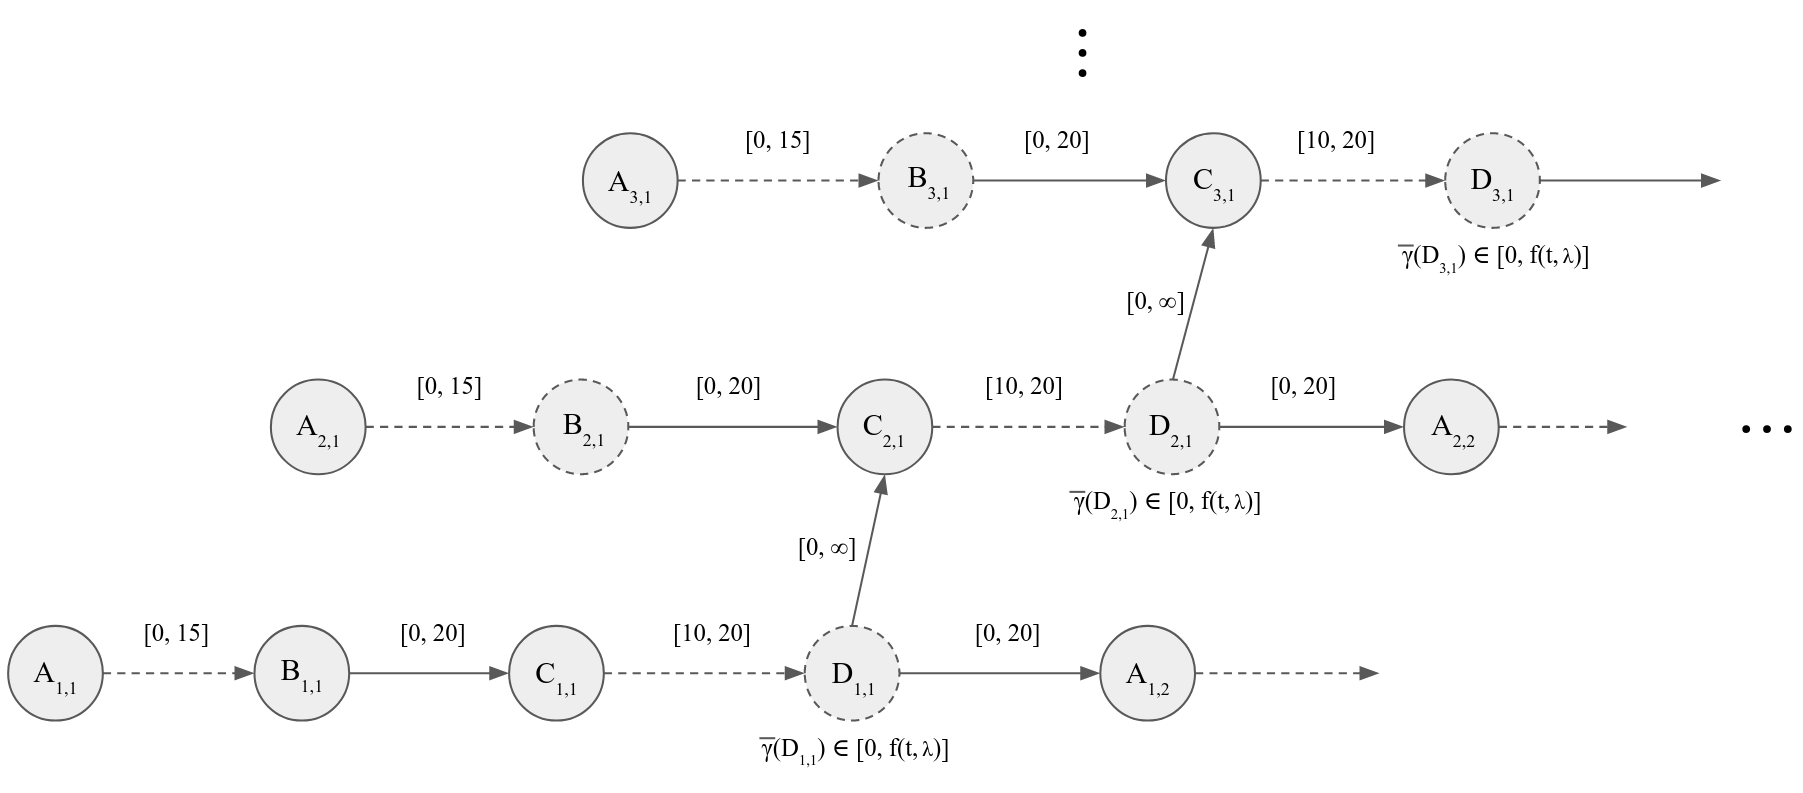
\includegraphics[width=1\textwidth]{images/dish-install-stnu.png}
\caption{\label{fig:dish-stnu}An STNU representing the installation and test of repeater antennas. Each row represents a single astronaut. The episode durations are representative of the bounds used in simulation.}
\end{figure}

we introduce an example which models a construction task on the lunar surface. This scenario depicted with the STNU in Figure \ref{fig:dish-stnu} represents an EVA wherein \(i\) astronauts are each installing \(j\) surface signal repeater antennas. During the activity, every astronaut is responsible for installing one repeater. \%Each event, \(X\), is represented for the \$i\$-th astronaut and \$j\$-th repeater as \(X_{i,j}\).

The astronauts work in parallel, with a \([0, \infty)\) requirement link from the start of the STNU to each \(A_{i,1}\) (not shown). The first episode, \(\conedge{A_{i,j}}{B_{i,j}}{}\), represents traversing to the site of the installation. We model traverses as uncontrollable due to the fact that crews are embarking across unknown terrain. Once at the site, an antenna is installed as represented by \(\edge{B_{i,j}}{C_{i,j}}{}\). Each repeater needs to have its configuration tested and confirmed working by \(D_{i,j}\), represented by the edge \(\conedge{C_{i,j}}{D_{i,j}}{}\). Confirmation takes the form of a request-response cycle to the ground. We model \(D_{i,j}\) as uncontrolled and with variable delay because each antenna takes an unknown time to self-configure and the crew does not know when they will receive a response from MCC that the repeater installation has been verified due to uncertainty in communication. Bandwidth is limited, so we limit the number of repeaters simultaneously sending requests to their configuration. We use the \(\edge{D_{i,j}}{C_{i+1,j}}{}\) links to enforce that the start of the confirmation of the next repeater does not begin until after the previous repeater's confirmation. Confirmations are required until we reach the last crew member or the last activity. Once testing is complete, the astronauts clean up their workstations, \(\edge{D_{i,j}}{A_{i,j+1}}{}\) and then repeat the cycle until all antennas have been installed.

\chapter{Coordinating Multiple Agents under Uncertain Communication}
\label{sec:orga6297c9}
\label{ch:technical-coordination}

In this chapter, we present a novel MA framework for dynamic event scheduling with inter-agent
temporal constraints. Our framework adheres to the variable observation delay modeling framework
presented in Chapter \ref{ch:modeling-tn}, making it robust to uncertain communication.

Online MA coordination of event dispatching allows executives to dynamically decide when to act
given the resolution of inter- and intra-agent temporal constraints. In our formulation, each
executive has its own STNU with contingent events it expects to observe and free events it is
responsible for monitoring. We do not distinguish between contingent events that are the free events
scheduled by peer agents and contingent events from any other source in Nature. There are no
restrictions on inter-agent constraints, though they must avoid chained contingencies the same way
that vanilla, single-agent STNUs do \citeprocitem{25}{[25]}.

We set forth the following requirements for the framework we contribute in this thesis.

\begin{itemize}
\item Executives are \emph{not} required to have perfect knowledge of the complete state of the world, nor
are they required to even \emph{agree} on the state of the world. Rather, their knowledge should be
consistent with the temporal constraints and observation delay modeled in their individual STNUs.
\item Executives are allowed to ignore observations.
\item \emph{All} inter-agent communications must be explicitly modeled.
\end{itemize}

To our knowledge, no such online scheduler for MA coordination has been proposed. In this chapter,
we first present a grounded Artemis-like scenario to motivate coordination. Next, we describe a
modeling framework for MA control programs that is necessary for establishing coordination between
agents. Next, we define an event propagation algorithm used to guarantee that event observations
match individual agent STNUs. We finish by presenting experimental analysis of our event propagation
algorithms, and the results of hardware demonstrations of Delay Kirk using a robotic arm and a
simulated astronaut.

\section{Motivating Scenario from EVAs}
\label{sec:orgd5fe304}

We envision a scenario with an astronaut and a robot coordinating on the lunar surface. The
astronaut is performing scientific exploration while the robot performs remote construction tasks.
The concept of operations allows for the astronaut to use a rover to traverse away from the robot in
search of promising scientific samples. Due to the position of surface relays and general
uncertainty in lunar topology, there is an uncertain time delay between agents.

Bandwidth between Mission Control on Earth and the Moon is limited. There are low and high bandwidth
communications available to both agents. Low bandwidth is responsible for transmitting critical data
(e.g. suit telemetry), while high bandwidth communications are reserved for purposes such as video
calls and large dumps of scientific data. It is not possible for both the astronaut and the robot to
use high bandwidth communications simultaneously. Thus, there is a need for the agents to coordinate
such that they make effective use of high bandwidth communications without stepping on each others
toes, so to speak.

We hone in on a point in an EVA where there is substantial time delay between the astronaut and
robot. The astronaut has set out far from the robot in search of scientifically interesting rock
samples. Meanwhile, the robot is preparing to perform a drilling operation. The astronaut's sample
collection work involves spectroscopy and video imagery, which is being sent to Mission Control
using the high bandwidth connection. It will take between 15 and 30 minutes to downlink all the
data. As soon as sample collection is over, the robot can use the high bandwidth connection to
perform a drilling operation.

We say that the astronaut ``owns,'' or is responsible for sharing observations of, the start and end
of the experiment, while the robot similarly owns the drilling operation.

\section{Multi-Agent Control Programs}
\label{sec:orga94f495}
\label{sec:ma-control-programs}

This thesis introduces challenges in writing control programs for multiple agents who need to
coordinate. We do not claim to solve all aspects of coordination, rather we present a framework for
simple scenarios with the key feature being that agents need to agree on the \emph{order} of a subset of
events. We start by presenting an example of inter-agent temporal constraints, followed by defining
a modeling framework for guaranteeing that agents agree about the order of events in their
respective partial histories. To the best of our knowledge, we are unaware of any other MA framework
for coordinating the order of event histories.

Consider two agents, \texttt{agent1} and \texttt{agent2}, that are scheduling STNUs \(S_{1}\) and \(S_{2}\)
respectively. \(S_{1}\) and \(S_{2}\) share a subset of semantically similar episodes, \(e_{1}\) and
\(e_{2}\). \texttt{agent1} ``owns'' \(e_{1}\), meaning it is responsible for scheduling the free event
\(e_{1}\)​-start and observing the contingent event \(e_{1}\)​-end, while \texttt{agent2} owns \(e_{2}\).

A simplified MA view of the constraints is as follows.

$$
\conedge{e_{1}\text{-start}}{e_{1}\text{-end}}{[15, 30]}
\edge{}{e_{2}\text{-start}}{[0, \infty]}
\conedge{}{e_{2}\text{-end}}{[22, 26]}
$$

From \texttt{agent1}'s perspective, \(S_{1}\) models the following constraints. We add a \texttt{noop} start event,
\(Z\), to simplify coordination.

$$
\edge{Z}{e_{1}\text{-start}}{[0, 0]}
\conedge{}{e_{1}\text{-end}}{[15, 30]}
\conedge{}{e_{2}\text{-start}}{[0, \infty]}
\conedge{}{e_{2}\text{-end}}{[22, 26]}
$$

\(S_{2}\) is then modeled as follows.

$$
\conedge{Z}{e_{1}\text{-start}}{[0, 0]}
\conedge{}{e_{1}\text{-end}}{[15, 30]}
\edge{}{e_{2}\text{-start}}{[0, \infty]}
\conedge{}{e_{2}\text{-end}}{[22, 26]}
$$

For the sake of controllability of \(S_{1}\) and \(S_{2}\), we would simply add \([0, 0]\) free
constraints between consecutive contingent constraints.

We will walk through scheduling this scenario from the perspective of both agents. First, we
describe their actions in the case that there is no communication delay, then we introduce the need
for communication, and finally we add delay to communications. This scenario will motivate our
analysis of the challenges that arise in MA control programs.

If both agents have perfect knowledge of the world (instantaneous knowledge of events), scheduling
is trivial. \texttt{agent1} and \texttt{agent2} execute \(Z\) simultaneously. \texttt{agent1} schedules \(e_{1}\)​-start and
\texttt{agent2} instantaneously receives an observation of \(e_{1}\)​-start. \(e_{1}\)​-end arrives in \([15, 30]\)
later, which again, both agents observe simultaneously. Now \texttt{agent2} is free to act. It schedules
\(e_{2}\)​-start, which \texttt{agent1} observes instantaneously. \(e_{2}\)​-end arrives \([22, 26]\) later and is
observed simultaneously by both agents.

Now, we enforce that \texttt{agent1} ``owns'' \(e_{1}\) and is the only agent that can observe it directly.
Likewise, \texttt{agent2} owns \(e_{2}\). In order for an agent to learn about an episode they do not own,
they must receive a communication from the agent who does. After \texttt{agent1} schedules \(e_{1}\)​-start,
it must send a message to \texttt{agent2}. \texttt{agent2} receives said message, which it interprets as an
observation of \(e_{1}\)​-start. If communications are instantaneous, the partial histories of both
agents agree on the assignment of \(e_{1}\)​-start. Later \(e_{1}\)​-end is observed by \texttt{agent1}, who is
then responsible for relaying a communication to \texttt{agent2} indicating that it is safe to assign
\(e_{1}\)​-end. \texttt{agent2} is now free to schedule \(e_{2}\)​-start, and follows the same pattern of sending
messages that events have been scheduled to \texttt{agent1}. After all events have been scheduled, the
histories of \texttt{agent1} and \texttt{agent2} still agree on the times assigned to each event.

We now show that adding delay to the communications between agents forces us to add \emph{synthetic}
episodes to \(S_{1}\) and \(S_{2}\) to maintain event ownership. We now say that for \(S_{2}\),
\(\gammabar(e_{2}\text{-end}) = [5, 15]\). In other words, \texttt{agent2} learns that \texttt{agent1} has finished
\(e_{2}\) some time in \([5, 15]\) after \texttt{agent1} has made the same assignment.

Once again, \texttt{agent1} schedules \(e_{1}\)​-start and sends a message to \texttt{agent2}. Unlike before, their
partial histories no longer match because \texttt{agent2} will assign \(e_{1}\)​-start to some time in \([5,
15]\) after \texttt{agent1}.

Adding communication introduces a coordination challenge, even when said communication is
instantaneous. Once again, we assume both agents execute \(Z\) simultaneously. When \texttt{agent1} schedules
\(e_{1}\)​-start, it must take the additional

We define coordination as sharing an understanding of when their peers have scheduled a subset of
events. To maintain consistency, we need to maintain the order of events. i.e.

\section{Event Propagation}
\label{sec:org51abd7d}
\label{sec:event-propagation}

At a high level, scheduled events propagate through a simple directed graph of connected executives.
We put checks in place to ensure that cycles do not cause infinitely recursed event observations.

\begin{defn}
\label{def:communication-graph}
\textbf{Communication Graph}

A \emph{communication graph} \(C\) is a tuple \(\langle V, E \rangle\), where:
\begin{itemize}
\item \(V\) is a set of vertices representing peer executives,
\item \(E\) is a set of directed edges between \(v \in V\) representing the path of event observation
propagation,
\item Each edge \(e_{i} \in E\) is a pair \((o, t)\), where \(o, t \in V\) represent the origin and
termination of the edge respectively.
\end{itemize}

Loops, or self-edges, are not allowed, i.e. for any vertex \(v_{i} \in V\), no single edge \(e_{i} \in
E\) may both originate and terminate at \(v_{i}\).
\end{defn}

For some executive \(v_{i} \in V\) with outgoing edges in \(E\), \((v_{i}, v_{j})\), \(\cdots\), \((v_{i},
v_{k})\), any scheduled events that \(v_{i}\) assigns, whether free or contingent, are propagated to
all peer executives \(v_{j}\), \(\cdots\), \(v_{k}\). Likewise, all contingent events received from Nature
are propagated to peers. Finally, any events \(v_{i}\) receives from other agents are also relayed to
peers.

\begin{defn}
\label{def:event-propagations}
\textbf{Event Propagation Messages}

An \emph{event propagation message} \(m\) is a tuple \(\langle x, P \rangle\), where:
\begin{itemize}
\item \(x\) is a set of one or more events scheduled simultaneously,
\item \(P \subseteq V\) is a set of executives who have already received the message.
\end{itemize}
\end{defn}

Recognize that Definition \ref{def:event-propagations} is vague in defining \(x\). Event propagation
messages are passed between agents, and each agent has its own STNU. In some cases, \(x\) will be free
events, in others \(x\) will be contingent events. The type of event makes no difference to the
algorithm so we do not distinguish between them here.

Events that are received in \(m\), \(m[x]\), are handled the same as observations of contingent events
during scheduling. Lemmas \ref{lemma:information-fixes-bounds}, \ref{lemma:ignore-inf-delay}, and
\ref{lemma:subtract-gamma} are applied as appropriate when the observation of \(m[x]\) arrives.

For an edge \((v_{i}, v_{j}) \in E\), it is possible that \(v_{j}\) receives events that are not present
in its STNU.

Because we have not defined a temporal decoupling-like algorithm wherein an STNU for multiple-agents
is programmatically separated into individual STNUs (see the discussion of multi-agent STNUs
\citeprocitem{40}{[40]} in Section \ref{sec:mastnus}), we are reliant on human planners to write STNUs for
each agent by hand. As a result, there is no guarantee that \(x\) is meaningful to a given agent.

To be more specific, there is no guarantee that any event \(x_{i} \in x\) in the event propagation
message has an equivalent event in \(X_{c}\) of the STNU being executed by any receiving agent \(v_{j}
\in V\). If agent \(v_{j}\) cannot find \(x_{i}\) in their \(X_{c}\), then \(x_{i}\) can be ignored. As will
be discussed in Algorithm \ref{alg:event-propagation}, we represent \(x\) using a type that can be compared
for equivalence with the events in an agent's STNUs, e.g. a list of strings.

We use \(P\) to avoid cycles in event propagation. As will be shown in Algorithm
\ref{alg:event-propagation}, agent \(v_{i}\) will avoid propagating \(x\) to any agents in \(P\). Agent \(v_{i}\)
will also grow \(P\) when it relays \(m\) to other agents by appending to \(P\) itself and all outgoing
agents \(v_{j}, \cdots, v_{k}\).

Timing information, e.g. timestamps, is explicitly excluded from \(m\). Dynamic scheduling and the
variable-delay STNU and event observation, \(\obs\), formalisms do not account for timestamps.
Instead, we expect that passing messages for event propagation between executives takes an amount of
time in the domain \(\mathbb{R^{+}}\). Thus, when \(v_{j}\) expects to receives an event, \(x_{i} \in x\),
from \(v_{i}\), the time delay can be naturally modeled in the variable-delay function,
\(\gammabar({x_{i}})\), in the STNU that \(v_{j}\) will execute.

If event propagation messages were to include accurate timestamps, we would need to modify the way
events are recorded during scheduling, impacting scheduling Lemmas \ref{lemma:information-fixes-bounds},
\ref{lemma:ignore-inf-delay}, and \ref{lemma:subtract-gamma}. Scheduling events in the past could also impact
controllability. For these reasons, we avoid the inclusion of timestamps in event propagation
messages.

By Definition \ref{def:event-propagations}, events received from other agents are no different than events
received from Nature, and no special considerations are required for scheduling.

We now walk through the process of passing messages between agents as shown in Algorithm
\ref{alg:event-propagation}. We use the same \emph{Event Propagation} algorithm in three cases:

\begin{enumerate}
\item When an agent \(v_{i}\) schedules free events \(x\),
\item When \(v_{i}\) receives an observation from Nature of contingent events \(x\),
\item When \(v_{i}\) receives an incoming message \(m_{i}\) with contingent events \(m_{i}[x]\) from another
agent in \(V\).
\end{enumerate}

Let \texttt{peers} be a mutable set initialized to the terminal vertices for all \(e \in E\) originating at
\(v_{i}\).

In the first case, agent \(v_{i}\) fulfills its responsibilities as defined in \(C\) by broadcasting \(x\)
to its \texttt{peers}, who will receive \(x\) as exogenous contingent events. The outgoing message \(m_{o}\)
that will be passed to \texttt{peers} will include enough information such that no agent should receive a
given \(x\) more than once. To do so, we let \(P\) be a set of all agents that will have observed \(x\)
when \(m_{o}\) is received by \texttt{peers}, \(P = \{ v_{i}, p~ \forall~ p \in \texttt{peers} \}\). We
finalize \(m_{o} = \langle x, P \rangle\), which we simultaneously transmit to each \(p\) in \texttt{peers}.
Transmission is a ``fire and forget'' operation, where \(v_{i}\) does not wait for acknowledgment from
any \(p\) that \(m_{o}\) was received.

The second case plays out the same as the first, the only difference being that \(x\) is itself
observed from Nature. Once again, we let \(P\) be a list of \(v_{i}\) and all \texttt{peers}, and then transmit
\(m_{o}\) simultaneously to all \texttt{peers}.

The third case is a relay operation. Agent \(v_{i}\) is responsible for propagating events \(m_{i}[x]\)
that it has just observed, but we want to avoid sending the events to \texttt{peers} who have already
observed them. We remove those agents from \texttt{peers} accordingly with a set difference operation:
\texttt{peers} \(= \texttt{peers} - m_{i}[P]\). Likewise, we grow the list of agents who have received \(x\),
which is now \(P = P \cup \texttt{peers}\). Agent \(v_{i}\) composes a new \(m_{o} = \langle m_{i}[x], P
\rangle\) and transmits it to \texttt{peers}.

Ideally, the Event Propagation algorithm should run on a separate thread from the main scheduling
loop, else we run the risk of incurring unnecessary delays in observing and dispatching events.

\begin{algorithm}
\SetAlgoLined
\SetKwComment{Comment}{/*}{*/}
\SetKwFunction{Return}{return}
\SetKwInput{Input}{Input}
\SetKwInput{Algorithm}{\textsc{Event Propagation}}
\SetKwInput{Initialize}{Initialization}
\SetKwIF{If}{ElseIf}{Else}{if}{then}{else if}{else}{endif}

\Indm
\Input{Incoming message $m_{i}$; Scheduled events $x$; Self $v_{i} \in V$; Set of outgoing $\texttt{peers} \subset V$}

\Indp
\Algorithm{}
\Indp

$\texttt{peers} \gets \texttt{peers} - m_{i}[P]$\;

$P \gets \{ m_{i}[P] \} \cup \{ v_{i} \} \cup \texttt{peers}$\;

$x \gets x$ or $m_{i}[x]$\;

$m_{o} \gets \langle x, P \rangle$\;

\For{each $p$ in $\texttt{peers}$} {
    Perform a non-blocking transmission of $m_{o}$ to $p$\;
}

\caption{An event propagation algorithm that avoids recursive message passing.}
\label{alg:event-propagation}
\end{algorithm}

The complexity of Algorithm \ref{alg:event-propagation} is trivially \(O(N)\), where \(N\) is the number of
executives in \(V - 1\). The limiting factor to the performance of Event Propagation will be the time
it takes to transmit messages between agents, which, to reiterate, should be modeled in the delay
functions for any inter-agent temporal constraints.

\section{Experimental Analysis}
\label{sec:org7e020e7}
\label{sec:ma-experimental}

We performed two analyses of the Event Propagation algorithm. The first was a hardware demonstration
performed on a Barrett WAM manipulator in the MERS lab. The second is a massively multi-agent
simulation. Both will be described below.

\subsection{Hardware Demonstration}
\label{sec:org69191b0}

We built a demonstration of the motivating scenario of this thesis in our lab using a Barrett WAM
manipulator representing the robot, and Valve Steam Deck representing the astronaut.

Each agent has their own RMPL control program, which we include in Listings \ref{code:astronaut-rmpl} and
\ref{code:robot-rmpl}. Note that each control program is nearly identical. The control programs related to
the high bandwidth handoff, \texttt{human-downlink-science}, \texttt{sync}, and \texttt{robot-drilling}, are nearly
identical, differing in observation delay and whether the \texttt{sync} event is controllable. Adding
observation delay reflects uncertain communication between the agents, while the \texttt{sync} activity
serves to keep the STNUs of the agents aligned.

\begin{listing}[htbp]
\begin{minted}[]{lisp}
;;;; -*- Mode: common-lisp; -*-

(defpackage #:scenario1)

(in-package #:scenario1)

(define-control-program human-downlink-science ()
  (declare (primitive)
           (duration (simple :lower-bound 15 :upper-bound 30)
                     :contingent t)))

(define-control-program sync ()
  (declare (primitive)
           (duration (simple :lower-bound 5 :upper-bound 15
                             :min-observation-delay 0
                             :max-observation-delay 1)
                     :contingent t)))

(define-control-program robot-drilling ()
  (declare (primitive)
           (duration (simple :lower-bound 22 :upper-bound 26
                             :min-observation-delay 0
                             :max-observation-delay 2)
                     :contingent t)))

(define-control-program human-closeout ()
  (declare (primitive)
           (duration (simple :lower-bound 10 :upper-bound 30))))

(define-control-program main ()
  (with-temporal-constraint (simple-temporal :upper-bound 480)
    (sequence (:slack nil)
      (human-downlink-science)
      (sync)
      (robot-drilling)
      (human-closeout))))
\end{minted}
\caption{\label{code:astronaut-rmpl}The control program the astronaut uses while collecting and downlinking scientific data.}
\end{listing}

\begin{listing}[htbp]
\begin{minted}[]{lisp}
;;;; -*- Mode: common-lisp; -*-

(defpackage #:scenario1)

(in-package #:scenario1)

(define-control-program human-downlink-science ()
  (declare (primitive)
           (duration (simple :lower-bound 15 :upper-bound 30
                             :min-observation-delay 5
                             :max-observation-delay 15)
                     :contingent t)))

(define-control-program sync ()
  (declare (primitive)
           (duration (simple :lower-bound 5 :upper-bound 15))))

(define-control-program robot-drilling ()
  (declare (primitive)
           (duration (simple :lower-bound 22 :upper-bound 26
                             :min-observation-delay 0
                             :max-observation-delay 1)
                     :contingent t)))

(define-control-program robot-poweroff ()
  (declare (primitive)
           (duration (simple :lower-bound 10 :upper-bound 30))))


(define-control-program main ()
  (with-temporal-constraint (simple-temporal :upper-bound 480)
    (sequence (:slack nil)
      (human-downlink-science)
      (sync)
      (robot-drilling)
      (robot-poweroff))))
\end{minted}
\caption{\label{code:robot-rmpl}The control program the robot uses to decide when to act with respect to learning the astronaut has finished collecting scientific data.}
\end{listing}

\subsection{Massively Multi-Agent Simulation}
\label{sec:orgdcede7b}

\chapter{An Architecture for Robust Scheduling and Dispatching}
\label{sec:orgfcf75fd}

\section{Clock-Synchronized Dispatching and Monitoring}
\label{sec:org8c77095}

In this section, we propose an architecture for organizing and executing long-running tasks in an
autonomous executive.

As described in Section \ref{sec:event-dispatching}, the dispatching algorithm should loop uninterrupted
until all executable events have been scheduled. There are, however, other tasks that an executive
needs to perform during execution, ranging from mission critical monitoring of contingent events, to
more mundane logging of debug and info-level messages to a human operator. Naturally, modern CPUs
and programming languages provide multi-threaded or multi-process applications to handle concurrent,
long-running tasks. While parallel computing is a perfectly viable option for building an executive,
we found that a clock-synchronized approach for long-running tasks more naturally aligns with our
autonomy reasoning abilities, and gives us more flexibility in the capabilities of Kirk.

\subsection{Challenges of Parallel Computing for Long-Running Tasks}
\label{sec:orgd78791d}

Consider the high-level responsibilities of Kirk, or any goal-based task and motion planner, during
execution. At a minimum, one must,

\begin{enumerate}
\item monitor progress towards its goals,
\item decide when to act,
\item send commands to hardware, and
\item communicate with a human operator.
\end{enumerate}

If we were to structure an executive based on these responsibilities, we may naturally start
allocating each responsibility to its own thread. Monitoring progress might be a loop that
constantly checks sensors or sensor-fused data. Deciding when to act would be the online dynamic
dispatching algorithm described in Section \ref{sec:event-dispatching}. We would not want hardware
commands to block dispatching, so we once again create a new thread. Meanwhile, the last thread
would collect information about the running executive, e.g. clock times, execution progress, and
explanations of the actions taken, in order to pass it along to a human operator.

While missions may take hours or days, simulations of said missions should take seconds. There are
many reasons to simulate. Before deploying an executive on expensive hardware in an extreme
environment, an operator may rightfully want to observe the behavior of the executive under a wide
range of potential mission conditions. Or we may want to try a new long-running task or motion
planning algorithm, but not want to wait hours to see how it performs. Or we may want to compare and
benchmark different options for task and motion planning. For these reasons and more, we need the
ability to reliably run an executive at faster than real-time speeds with confidence that its
behavior in simulation is reflective of its performance in the real-world. Thus, during simulation,
we add another responsibility:

\begin{enumerate} \setcounter{enumi}{4} \item
update the clock at faster than real-time speeds.
\end{enumerate}

Parallel computing starts to break down when we want to simulate a mission due to synchronization
challenges. For instance, the event monitoring thread may be waiting to simulate a contingent event
observation at time \(t\). We would need to ensure that the operation in the monitoring thread that
checks the clock time runs at least once while the clock is at \(t\). If the clock is running too
quickly, \(t\) could be missed and the simulated contingent event is never observed. We could make the
check more robust by either slowing the clock down or adding tolerance to the time check, e.g.
checking that the clock is within a range near \(t\) instead of exactly \(t\), but the underlying
problem remains.

There may also be temporal dependencies between threads. Algorithm \ref{alg:dispatcher-inner} assumes that
the time does not change while it is running. During real-time operations, it is effectively the
case that time is not passing, but we lose the guarantee in simulation. It could be that the
dispatcher believes it to be time \(t\) when it dispatches an event, but by the time the event is
scheduled or the driver receives a command, the clock is now at time \(t' \gg t\), impacting the
controllability of the STNU.

None of the problems introduced by parallel computing are insurmountable, but they add code and
complexity to an already complex system. This creates two fundamental concerns that caused us to
rewrite the online architecture of Kirk. First is that adding code \emph{post-hoc} to decision-making
algorithms to address special cases, like faster than real-time clocks, means that the code we
simulate and the code we run during missions fundamentally differ. This differentiation reduces our
confidence that testing and verifying the executive in simulation is indicative of its performance
in real-time. Second is that additional complexity increases the surface area for failures and
anomalous behavior. Instead, we propose a clock-based synchronization approach that is no less
efficient during real-time operations while requiring no change to our decision-making algorithms to enable
faster than real-time simulation.

\subsection{Clock-Based Synchronization}
\label{sec:org439dbf2}

Clock-based synchronization hands control of long-running tasks to a shared clock. Rather than
allowing each thread to run independently, the clock takes responsibility for executing tasks at an
appropriate interval. We call each interval a \emph{tick}.

At each tick, every \emph{task} (Definition \ref{def:task}) is run. Tasks are lambda functions that communicate
to the clock by their return values. If a task returns \texttt{true}, it is interpreted as a signal that
the clock may continue ticking. Returning \texttt{false} tells the clock that ticking should stop. So long
as all tasks want the clock to continue ticking, it should. If any task returns \texttt{false}, ticking
should stop.

\begin{defn}
\label{def:task}
\textbf{Task}

A \emph{task} is a lambda function that takes nothing as input and returns a Boolean. The return value
indicates whether the task wants the clock to continue ticking.
\end{defn}

Before the clock starts to run, the executive adds tasks to a queue. The tasks will be run
consecutively in the order they appear.

Implemented in a real-time clock, the ticking algorithm should run as fast as possible. We do so by
implementing Algorithm \ref{alg:realtime-clock-tick}, which recursively calls itself until it receives a
signal from a task that it should stop.

\begin{algorithm}
\SetAlgoLined
\SetKwComment{Comment}{//}{}
\SetKwFunction{Return}{return}
\SetKwInput{Input}{Input}
\SetKwInput{Output}{Output}
\SetKwInput{Algorithm}{\textsc{clockTick}}
\SetKwInput{Initialize}{Initialization}
\SetKwIF{If}{ElseIf}{Else}{if}{then}{else if}{else}{endif}

\Indm
\Input{Boolean $\mathit{tickp}$; Task queue $\mathit{queue}$;}

\Indp
\Algorithm{}
\Indp

\If{$\mathit{tickp} \land (\mathit{queue[length]} > 0)$} {
    \For{$\mathit{task}$ in $\mathit{queue}$} {
        $\mathit{tickp} \gets (\mathtt{task()} \land \mathit{tickp})$\;
    }
    $\mathtt{clockTick(\mathit{tickp}, \mathit{queue})}$
}

\caption{A recursive algorithm for clock-synchronized tasks in real-time.}
\label{alg:realtime-clock-tick}
\end{algorithm}

We simulate a faster than real-time clock with Algorithm \ref{alg:sim-clock-tick}. The key difference is
the additional clock advancement operation added before recursing. Unlike a synchronized thread
approach, we are guaranteed an order of operations between tasks and the clock. We know tasks will
run in the order they appear in \(\mathit{queue}\), the clock will advance, then the tasks will run
again.

\begin{algorithm}
\SetAlgoLined
\SetKwComment{Comment}{//}{}
\SetKwFunction{Return}{return}
\SetKwInput{Input}{Input}
\SetKwInput{Output}{Output}
\SetKwInput{Algorithm}{\textsc{clockTick}}
\SetKwInput{Initialize}{Initialization}
\SetKwIF{If}{ElseIf}{Else}{if}{then}{else if}{else}{endif}

\Indm
\Input{Boolean $\mathit{tickp}$; Task queue $\mathit{queue}$; Sleep duration $d$;}

\Indp
\Algorithm{}
\Indp

\If{$\mathit{tickp} \land (\mathit{queue[length]} > 0)$} {
    \For{$\mathit{task}$ in $\mathit{queue}$} {
        $\mathit{tickp} \gets (\mathtt{task()} \land \mathit{tickp})$\;
    }
    Advance clock by $d$\;
    $\mathtt{clockTick(\mathit{tickp}, \mathit{queue}, \mathit{d})}$
}

\caption{A recursive algorithm for clock-synchronized tasks in faster than real-time.}
\label{alg:sim-clock-tick}
\end{algorithm}

If Algorithms \ref{alg:realtime-clock-tick} and \ref{alg:sim-clock-tick} are implemented as class methods,
\(\mathit{tickp}\) naturally lends itself to be a class property. As such, other interfaces can be
built for controlling \(\mathit{tickp}\), ultimately leading to a robust clock that can be arbitrarily
started and stopped as required. In the implementation of Kirk for this thesis, this paradigm
enables us to perform time consuming offline planning upon its initialization, including tasks like
running the pipeline to go from RMPL to a distance graph, before starting the clock when we are
ready to start scheduling.

\section{Single-Responsibility Principle}
\label{sec:org43693bf}

Not an exact law but something we followed with scheduler > dispatcher > driver layers

\chapter{Evaluation}
\label{sec:org3506a58}

This is a chapter on evaluating all this stuff.

\chapter{Discussion and Future Work}
\label{sec:orgdc1a92e}

\section{Optimistic Rescheduling}
\label{sec:org786c406}
\label{sec:discussion-optimistic-rescheduling}

What if we looked for conflicts? Could we possibly search for a time to dispatch early in the
buffered execution space?

Smarter rewriting STNU. Could we update the existing d-graph directly and check it for SRNCs? maybe?

\section{Coordination}
\label{sec:org3d924fa}
\label{sec:mastnus}

We were focused on addressing the multi-agent (MA) online scheduling problem. Before scheduling, we
must contend with planning, e.g. building variable-delay STNUs for each agent. We considered
extending the two existing planning approaches described below to model variable observation delay
between agents. We ultimately decided neither were fit for the motivating scenarios of this thesis.
Instead, we used a manual planning approach more akin to the ISS EVA planning process.

The first planning approach we considered was to model the system as a Multi-Agent STNU (MASTNU)
\citeprocitem{40}{[40]}. MASTNUs allow modelers to describe temporal constraints between multiple
agents, then check the overall dynamic controllability of the system. To check the controllability
of a MASTNU, the first step is to perform temporal decoupling with the goal of producing individual
dynamically controllable STNUs for each agent that can be dynamically scheduled per usual. While
superficially promising, there is a considerable drawback to this approach, namely that temporal
decoupling is sound but not complete, i.e. temporal decoupling may report failure even when the
MASTNU is dynamically controllable. This limits the utility of MASTNUs as a planning tool.

The other approach to this problem we are aware of is Stedl's Hierarchical Reformulation (HR)
algorithm \citeprocitem{41}{[41]}. HR begins with a MA temporal plan network (TPN), which is similar to a
MASTNU (though HR pre-dates MASTNUs). Stedl's key insight is to avoid inter-agent communication
altogether by reformulating constraints between groups of agents such that they are strongly
controllable. As such, no communication between agents is required. A centralized dispatcher is then
responsible for then handing events to agents. We also assume that there is no central authority,
making HR a poor fit for our problem domain.

Both MASTNUs and HR assume communications between agents are either instantaneous or impossible,
i.e. with an infinite delay. As we will see in Section \ref{sec:vdc}, our formalism for variable
observation delay allows a \emph{spectrum} of communication delay. While we felt it was possible to
shoehorn uncertain observation delay into MASTNUs or HR, we felt both were a poor choice because of
their pre-existing expectations with respect to communication. In combination with our focus on
online scheduling, we decided to forgo extending either formalism to account for observation delay.
Instead our planning process simply consists of manually writing variable-delay STNUs with
intra-agent and inter-agent temporal constraints by hand.

We believe it may be possible for MASTNUs or HR to be expanded to include variable observation
delay, though we leave that problem for future research.

We considered framing our approach to inter-agent communication as a distributed consensus problem
because we believed we needed a means for disparate agents to agree on the state of the world.
Existing distributed consensus algorithms like Paxos \citeprocitem{42}{[42]} or Raft \citeprocitem{43}{[43]}
would then be integrated into the communication layer of Kirk and take responsibility for ensuring
that agents agree on which events have been scheduled.

Ultimately the drawbacks of a distributed consensus approach outweighed the benefits. Chiefly, both
Paxos and Raft assume that communications are either instantaneous and freely available or that
agents have gone dark (i.e. can no longer communicate). This communication model is incongruous with
the explicitly modeled communications of the VDC formalism. Furthermore, the VDC formalism allows us
to model that agents never receive communications, negating the requirement for distributed
consensus.

\appendix

\chapter{Comparison of Variable-Delay STNUs to Partially Observable STNUs}
\label{sec:org494cf65}
\label{appendix:postnus}

The delay scheduler is flexible in that so long as it receives a variable-delay STNU, it is capable
of scheduling. Human modelers have flexibility in how they represent temporal constraints in that
there are many flavors of STNUs, each with their own advantages and disadvantages. Earlier, we
presented RMPL as a modeling language that is compiled to variable-delay STNUs. There are other
choices for modeling frameworks. Here, we present a comparison of variable-delay STNUs to POSTNUs
\citeprocitem{32}{[32]}, a flavor that is similar in many respects. This section presents a comparison
of variable-delay STNUs and POSTNUs, including transformations that allow some classes of POSTNUs to
be represented as variable-delay STNUs.

One of the strengths of the variable-delay controllability model is its ability to generalize the
concepts of strong and dynamic controllability. This technique was first seen in greater depth in
the context of POSTNUs. In an STNU, all contingent events are either
instantaneously observable under a dynamic controllability model or entirely unobservable under a
strong controllability model. In POSTNUs, contingent events can be marked observable and
unobservable. To say that a POSTNU is dynamically controllable equates to asserting that it is
possible to construct a schedule during execution that respects all constraints if the scheduler
only receives information about observable contingent events.

While, superficially, POSTNUs and delay STNUs appear to model distinct problems in temporal
reasoning, all delay STNUs can be accurately represented as POSTNUs. While the converse is not true,
there is a subset of POSTNUs that delay STNUs are able to model. It is advantageous to translate
POSTNUs to delay STNUs when possible because we are guaranteed to finish controllability checks for
delay STNUs in polynomial time, while evaluating the controllability of POSTNUs in general is harder
\citeprocitem{32}{[32]}. Furthermore, the sub-class of POSTNUs that can be checked efficiently and
accurately, those without chained contingent links \citeprocitem{44}{[44]}, are members of the
subset of POSTNUs that can be expressed directly as STNUs with fixed-delay, and likewise
variable-delay, functions , \citeprocitem{31}{[31, p. 59]}. The converse is also true - we may emulate
STNUs with variable-delay functions as POSTNUs without chained contingent links. Below, we elaborate
on translations from delay STNUs to POSTNUs, before describing how we can express POSTNUs without
chained contingent links as STNUs with fixed-delay functions. Note that this is not a comprehensive
list of transformations between delay STNUs and POSTNUs - our aim is to describe the minimum set of
transformations required to model POSTNUs without chained contingent links as delay STNUs. For the
following discussion, let \(S\) be a delay STNU and \(P\) be an equivalent POSTNU.

We present these transformations to demonstrate that the delay scheduler is capable of scheduling
POSTNUs without chained contingencies. So long as it receives a variable-delay STNU, the fact that
POSTNUs can be scheduled allows modelers additional flexibility in their means of representing the
problem domain.

We start with an \(S\) that consists of the links \(\conedge{A}{B}{}\) and \(\edge{B}{D}{}\) with delay
function \(\gammabar(B)\). See Figure \ref{fig:postnu} for an example translation between a fixed-delay STNU
and a POSTNU.

\begin{lemma}
\label{lemma:delay-stnu-to-postnu}
For contingent link \(\conedge{A}{B}{}\) in \(S\) with observation delay \(\gammabar(B) = [l, u]\), where
\(0 \leq l \leq u < \infty\), and outgoing requirement link \(\edge{B}{D}{}\), we may emulate
observation delay in \(P\) by copying \(\conedge{A}{B}{}\) and \(\edge{B}{D}{}\) to \(P\), enforcing that
\(B\) is unobservable, and adding a new observable contingent event, \(B'\) with \(\conedge{B}{B'}{[l,
u]}\).
\end{lemma}

\begin{proof}
In both \(S\) and \(P\), we do not observe \(B\) directly, yet we define an outgoing requirement link,
\(\edge{B}{D}{}\), that depends entirely on the resolution of \(B\). The only information available to
reason about the assignment of \(B\) comes in the form of an indirect observation, \(B'\) or
\(\gammabar(B)\), received after a delay in \(\mathbb{R}^{\geq 0}\). If \(P\) was not equivalent to \(S\),
we would be able to learn the assignment of \(B\) without waiting \(\gammabar(B)\) time units after its
true assignment. Thus, because we must wait \(B' - B \in [l, u]\) time units to learn the assignment
of \(B\), and \(\edge{B}{D}{}\) has equivalent constraints between \(S\) and \(P\), \(P\) must model the same
semantics as \(S\).
\end{proof}

\begin{lemma}
\label{lemma:postnu-observable}
For a contingent event \(B\) with variable-delay function \(\gammabar(B) = [0, 0]\) in \(S\), we may
emulate the same constraints with an observable contingent event, \(B\) in \(P\).
\end{lemma}

\begin{proof}
The variable-delay function enforces instantaneous observation. By the definition of observable
contingent events in the POSTNU model, we will observe \(B\) instantaneously.
\end{proof}

A POSTNU with a chained contingency is defined as follows. Consider a chain of contingent events,
\(\conedge{A}{B}{}\) and \(\conedge{B}{C}{}\). If \(B\) has one or more outgoing links to free or
contingent events other than \(C\), it is a chained contingency. Lemma \ref{lemma:delay-stnu-to-postnu}
results in a POSTNU without chained contingencies, hence variable-delay STNUs fall into the subclass
of POSTNUs that can be checked efficiently \citeprocitem{44}{[44]}.

In the other direction, to transform a POSTNU without chained contingencies into an STNU with
variable-delay functions, we need to address three cases of contingent constraints: (1) unobservable
contingent events not immediately followed by other contingent constraints, (2) unobservable
contingent events immediately followed by other contingent constraints, and (3) observable
contingent constraints.

\begin{lemma}
\label{lemma:postnu-unobservable}
For an unobservable event \(B\) in \(P\), with no outgoing contingent links, we can emulate it in \(S\)
with a contingent event \(B\) and upper bound of its variable-delay function set to \(\gammabar^+(B) =
\infty\).
\end{lemma}

\begin{proof}
We will not observe \(B\) nor will outgoing contingent links provide information about \(B\). As such we
define \(\gammabar^+(B) = \infty\) in \(S\).\footnote{Note: ,p. \citeprocitem{31}{[31, p. 60]} erroneously claims
that we should define \(\gamma(B) = 0\) for unobservable events.} From a controllability standpoint
for both \(S\) and \(P\), we know the \emph{a priori} bounds of \(B\) but will not learn its true assignment.
\end{proof}

\begin{lemma}
\label{lemma:combine-postnu-ctg}
For an unobservable contingent link \(\conedge{A}{B}{[m, n]}\) in \(P\), with a single outgoing link,
\(\conedge{B}{C}{[w, z]}\), we replace the two constraints from \(P\) in \(S\) with a concatenated
constraint, \(\conedge{A}{C}{[m+w, n+z]}\).
\end{lemma}

\begin{proof}
The only information we may receive is the observation of \(C\). Given there are no other outgoing
links from \(B\), folding \(B\) into the successive contingent constraint can not affect the semantics
of the network. The bounds of the new link, \(\conedge{A}{C}{[m + w, n + z]}\) is the result of
summing the intervals of \(\conedge{A}{B}{[m, n]}\) and \(\conedge{B}{C}{[w, z]}\): \([m, n] + [w, z] =
[m + w, n + z]\).
\end{proof}

Note that we did not specify whether \(C\) is observable in \(P\). After applying Lemma
\ref{lemma:combine-postnu-ctg}, we then apply either Lemma \ref{lemma:postnu-observable} or
\ref{lemma:postnu-unobservable} to \(C\).

\begin{lemma}
For an observable contingent event \(\conedge{A}{B}{[m, n]}\) in \(P\), with a single outgoing link to
an observable contingent event, \(C\), \(\conedge{B}{C}{[w, z]}\), we create three constraints in \(S\):
\(\conedge{A}{B}{[m, n]}\), \(\edge{B}{B'}{[0, 0]}\), and \(\conedge{B'}{C}{[w, z]}\) where \(\gammabar(B)
= [0, 0]\).
\end{lemma}

\begin{proof}
Given \(C\) is observable in \(P\), a simulated free event, \(B'\) in \(S\), can be scheduled simultaneously
with \(B\). Any contingent constraints following \(B\) now start at an executable event and are thus
valid constraints in \(S\). \(B\) is observable, so we need no observation delay according to Lemma
\ref{lemma:postnu-observable}.
\end{proof}

Thus, delay STNUs are sufficiently capable of expressing all POSTNUs that can efficiently be checked
for controllability using today's tractable POSTNU algorithms.

\begin{figure}[!htb]
\label{fig:postnu}
\caption{(a) An STNU with a contingent constraint that has a certain delay. (b) One possible way of rewriting the STNU as an equivalent POSTNU. This particular POSTNU exhibits a chained contingency, as $B$ is a contingent event that starts a contingent constraint and is connected to $B'$ via a contingent constraint.}
\centering
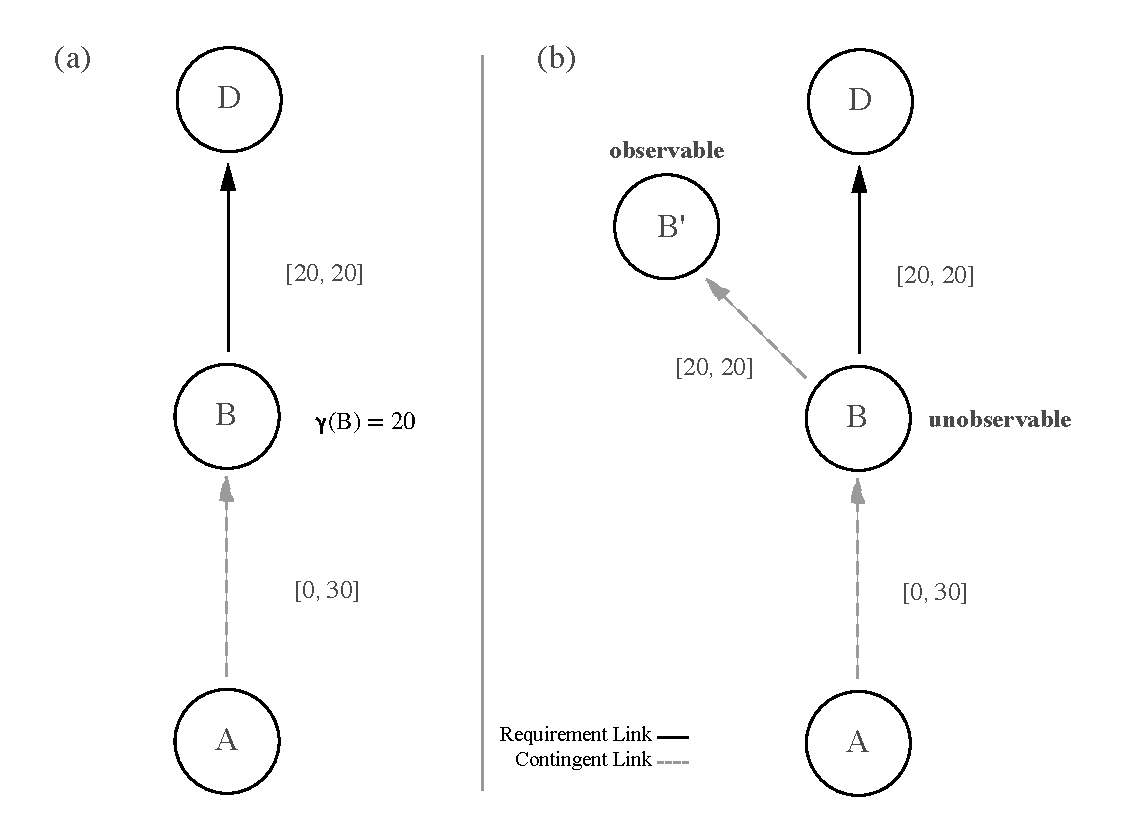
\includegraphics[width=0.75\textwidth]{POSTNU.pdf}
\end{figure}

It is not clear if controllability can be checked more efficiently across a greater subset of
POSTNUs beyond those without chained contingencies. However, it is worth highlighting that
variable-delay controllability can be leveraged to construct improved algorithms with respect to
scheduling and controllability of POSTNUs. The model for observation delay proposed by
variable-delay controllability can be expressed exactly as a POSTNU with a ``single-headed'' chained
contingency\footnote{To borrow the term ``single-headed'' from \citeprocitem{45}{[45]}.} as shown
in Figure \ref{fig:postnu}b; the main difference is that we represent the contingent link between \(B\) and
\(B'\) with our variable-delay function \(\gammabar(B)\). Hence, the algorithm we present for
variable-delay controllability can be used to both solve POSTNUs without chained contingencies, as
described above, as well as those POSTNUs with single-headed chained contingencies. Approaches
inspired by variable-delay controllability have been used to further expand POSTNU dynamic
controllability checking in more expressive chained instances \citeprocitem{45}{[45]}. We
hope that insights from variable-delay controllability will continue to expand the subset of POSTNUs
that can be controllability checked, and as such we advocate for continued development of the theory
of variable-delay controllability as a relevant framework for modelers.

%% This defines the bibliography file (main.bib) and the bibliography style.
%% If you want to create a bibliography file by hand, change the contents of
%% this file to a `thebibliography' environment.  For more information
%% see section 4.3 of the LaTeX manual.
\bibliography{extra-citations}
\begin{singlespace}
\begin{thebibliography}

\begin{hangparas}{1.5em}{1}
\hypertarget{citeproc_bib_item_1}{[1] N. Bhargava, C. Muise, and B. C. Williams, “Variable-delay controllability,” in \textit{IJCAI International Joint Conference on Artificial Intelligence}, 2018, vol. 2018-July, pp. 4660–4666. doi: \href{https://doi.org/10.24963/ijcai.2018/648}{10.24963/ijcai.2018/648}.\\}

\hypertarget{citeproc_bib_item_2}{[2] M. J. Miller, “Decision Support System Development For Human Extravehicular Activity,” Georgia Institute of Technology, 2017.\\}

\hypertarget{citeproc_bib_item_3}{[3] D. Wang and B. C. Williams, “TBurton: A divide and conquer temporal planner,” in \textit{Proceedings of the National Conference on Artificial Intelligence}, 2015, vol. 5, pp. 3409–3417.\\}

\hypertarget{citeproc_bib_item_4}{[4] J. W. McBarron, “Past, present, and future: The U.S. EVA Program,” \textit{Acta astronautica}, vol. 32, no. 1, pp. 5–14, 1994, doi: \href{https://doi.org/10.1016/0094-5765(94)90143-0}{10.1016/0094-5765(94)90143-0}.\\}

\hypertarget{citeproc_bib_item_5}{[5] C. P. Sonnett, “REPORT of the AD HOC WORKING GROUP ON APOLLO EXPERIMENTS AND TRAINING on the SCIENTIFIC ASPECTS OF THE APOLLO PROGRAM,” NASA, 1963.\\}

\hypertarget{citeproc_bib_item_6}{[6] J. M. Hurtado, K. Young, J. E. Bleacher, W. B. Garry, and J. W. Rice, “Field geologic observation and sample collection strategies for planetary surface exploration: Insights from the 2010 Desert RATS geologist crewmembers,” \textit{Acta astronautica}, vol. 90, no. 2, pp. 344–355, 2013, doi: \href{https://doi.org/10.1016/j.actaastro.2011.10.015}{10.1016/j.actaastro.2011.10.015}.\\}

\hypertarget{citeproc_bib_item_7}{[7] K. Young and T. Graff, “Planetary Science Context for EVA,” in \textit{NASA EVA Exploration Workshop}, 2020, p. 40.\\}

\hypertarget{citeproc_bib_item_8}{[8] A. Kanelakos, “Artemis EVA Flight Operations - Preparing for Lunar EVA Training \& Execution,” in \textit{NASA EVA Exploration Workshop}, 2020, p. 47.\\}

\hypertarget{citeproc_bib_item_9}{[9] C. Campbell, “Advanced EMU Portable Life Support System (PLSS) and Shuttle/ISS EMU Schematics, a Comparison,” \textit{42nd international conference on environmental systems}, pp. 1–18, 2012, doi: \href{https://doi.org/10.2514/6.2012-3411}{10.2514/6.2012-3411}.\\}

\hypertarget{citeproc_bib_item_10}{[10] E. S. Patterson and D. D. Woods, “Shift changes, updates, and the on-call architecture in space shuttle mission control,” \textit{Computer supported cooperative work}, vol. 10, no. 3-4, p. 27, 2001, doi: \href{https://doi.org/10.1023/A:1012705926828}{10.1023/A:1012705926828}.\\}

\hypertarget{citeproc_bib_item_11}{[11] S. J. Payler \textit{et al.}, “Developing Intra-EVA Science Support Team Practices for a Human Mission to Mars,” \textit{Astrobiology}, vol. 19, no. 3, pp. 387–400, 2019, doi: \href{https://doi.org/10.1089/ast.2018.1846}{10.1089/ast.2018.1846}.\\}

\hypertarget{citeproc_bib_item_12}{[12] D. A. Coan, “Exploration EVA System Concept of Operations Summary for Artemis Phase 1 Lunar Surface Mission,” NASA, Houston, TX, 2020.\\}

\hypertarget{citeproc_bib_item_13}{[13] M. A. Seibert, D. S. Lim, M. J. Miller, D. Santiago-Materese, and M. T. Downs, “Developing Future Deep-Space Telecommunication Architectures: A Historical Look at the Benefits of Analog Research on the Development of Solar System Internetworking for Future Human Spaceflight,” \textit{Astrobiology}, vol. 19, no. 3, pp. 462–477, Mar. 2019, doi: \href{https://doi.org/10.1089/ast.2018.1915}{10.1089/ast.2018.1915}.\\}

\hypertarget{citeproc_bib_item_14}{[14] M. J. Miller and K. M. Feigh, \textit{Addressing the envisioned world problem: A case study in human spaceflight operations}, vol. 5. Cambridge University Press, 2019. doi: \href{https://doi.org/10.1017/dsj.2019.2}{10.1017/dsj.2019.2}.\\}

\hypertarget{citeproc_bib_item_15}{[15] M. J. Miller, K. M. McGuire, and K. M. Feigh, “Information flow model of human extravehicular activity operations,” \textit{Ieee aerospace conference proceedings}, vol. 2015-June, 2015, doi: \href{https://doi.org/10.1109/AERO.2015.7118942}{10.1109/AERO.2015.7118942}.\\}

\hypertarget{citeproc_bib_item_16}{[16] M. J. Miller, K. M. McGuire, and K. M. Feigh, “Decision Support System Requirements Definition for Human Extravehicular Activity Based on Cognitive Work Analysis,” \textit{Journal of cognitive engineering and decision making}, vol. 11, no. 2, pp. 136–165, 2017, doi: \href{https://doi.org/10.1177/1555343416672112}{10.1177/1555343416672112}.\\}

NO\_ITEM\_DATA:Sehlke2019

\hypertarget{citeproc_bib_item_18}{[18] B. C. Williams, M. D. Ingham, S. H. Chung, and P. H. Elliott, “Model-based programming of intelligent embedded systems and robotic space explorers,” \textit{Proceedings of the ieee}, vol. 91, no. 1, pp. 212–236, 2003, doi: \href{https://doi.org/10.1109/JPROC.2002.805828}{10.1109/JPROC.2002.805828}.\\}

\hypertarget{citeproc_bib_item_19}{[19] B. C. Williams and R. J. Ragno, “Conflict-directed A* and its role in model-based embedded systems,” \textit{Discrete applied mathematics}, vol. 155, no. 12, pp. 1562–1595, 2007, doi: \href{https://doi.org/10.1016/j.dam.2005.10.022}{10.1016/j.dam.2005.10.022}.\\}

\hypertarget{citeproc_bib_item_20}{[20] R. E. Fikes and N. J. Nilsson, “Strips: A new approach to the application of theorem proving to problem solving,” \textit{Artificial intelligence}, vol. 2, no. 3-4, pp. 189–208, 1971, doi: \href{https://doi.org/10.1016/0004-3702(71)90010-5}{10.1016/0004-3702(71)90010-5}.\\}

\hypertarget{citeproc_bib_item_21}{[21] R. Dechter, I. Meiri, and J. Pearl, “Temporal constraint networks,” \textit{Artificial intelligence}, vol. 49, no. 1-3, pp. 61–95, 1991, doi: \href{https://doi.org/10.1016/0004-3702(91)90006-6}{10.1016/0004-3702(91)90006-6}.\\}

\hypertarget{citeproc_bib_item_22}{[22] E. Fernández González, “Generative Multi-Robot Task and Motion Planning Over Long Horizons,” Massachusetts Institute of Technology, 2018.\\}

\hypertarget{citeproc_bib_item_23}{[23] J. Chen, B. C. Williams, and C. Fan, “Optimal mixed discrete-continuous planning for linear hybrid systems,” in \textit{HSCC 2021 - Proceedings of the 24th International Conference on Hybrid Systems: Computation and Control (part of CPS-IoT Week)}, 2021, vol. 1. doi: \href{https://doi.org/10.1145/3447928.3456654}{10.1145/3447928.3456654}.\\}

\hypertarget{citeproc_bib_item_24}{[24] T. Vidal and H. Fargier, “Handling Contingency in Temporal Constraint Networks: From Consistency to Controllabilities,” \textit{Journal of experimental and theoretical artificial intelligence}, vol. 11, no. 1, pp. 23–45, 1999, doi: \href{https://doi.org/10.1080/095281399146607}{10.1080/095281399146607}.\\}

\hypertarget{citeproc_bib_item_25}{[25] P. H. Morris, N. Muscettola, and T. Vidal, “Dynamic Control Of Plans With Temporal Uncertainty,” 2001.\\}

\hypertarget{citeproc_bib_item_26}{[26] P. Morris and N. Muscettola, “Temporal dynamic controllability revisited,” \textit{Proceedings of the national conference on artificial intelligence}, vol. 3, pp. 1193–1198, 2005.\\}

\hypertarget{citeproc_bib_item_27}{[27] P. Morris, “A structural characterization of temporal dynamic controllability,” \textit{Lecture notes in computer science (including subseries lecture notes in artificial intelligence and lecture notes in bioinformatics)}, vol. 4204 LNCS, pp. 375–389, 2006, doi: \href{https://doi.org/10.1007/11889205\_28}{10.1007/11889205\\_28}.\\}

\hypertarget{citeproc_bib_item_28}{[28] P. Morris, “Dynamic controllability and dispatchability relationships,” \textit{Lecture notes in computer science (including subseries lecture notes in artificial intelligence and lecture notes in bioinformatics)}, vol. 8451 LNCS, no. Dc, pp. 464–479, 2014, doi: \href{https://doi.org/10.1007/978-3-319-07046-9\_33}{10.1007/978-3-319-07046-9\\_33}.\\}

\hypertarget{citeproc_bib_item_29}{[29] A. Cimatti, A. Micheli, and M. Roveri, “Solving temporal problems with uncertainty using SMT: Strong Controllability,” \textit{Constraints}, vol. 20, no. 1, pp. 1–29, 2012, doi: \href{https://doi.org/10.1007/s10601-014-9167-5}{10.1007/s10601-014-9167-5}.\\}

\hypertarget{citeproc_bib_item_30}{[30] M. Ingham, R. Ragno, A. Wehowsky, and B. Williams, “The Reactive Model-based Programming Language,” MIT Space Systems and Artificial Intelligence Laboratories, 2002.\\}

\hypertarget{citeproc_bib_item_31}{[31] N. Bhargava, “Multi-Agent Coordination under Limited Communication,” Massachusetts Institute of Technology, 2020.\\}

\hypertarget{citeproc_bib_item_32}{[32] M. D. Moffitt, “On the partial observability of temporal uncertainty,” \textit{Proceedings of the national conference on artificial intelligence}, vol. 2, pp. 1031–1037, 2007.\\}

\hypertarget{citeproc_bib_item_33}{[33] G. Kiczales, J. Des Rivières, and D. G. Bobrow, \textit{The art of the metaobject protocol}. Cambridge, Mass: MIT Press, 1991.\\}

\hypertarget{citeproc_bib_item_34}{[34] M. Fox and D. Long, “PDDL2.1: An extension to PDDL for expressing temporal planning domains,” \textit{Journal of artificial intelligence research}, vol. 20, pp. 61–124, 2003, doi: \href{https://doi.org/10.1613/jair.1129}{10.1613/jair.1129}.\\}

\hypertarget{citeproc_bib_item_35}{[35] N. Bhargava, C. Muise, T. Vaquero, and B. Williams, “Delay Controllability : Multi-Agent Coordination under Communication Delay,” Massachusetts Institute of Technology, Cambridge, MA, 2018.\\}

\hypertarget{citeproc_bib_item_36}{[36] L. Hunsberger, “Efficient execution of dynamically controllable simple temporal networks with uncertainty,” \textit{Acta informatica}, vol. 53, no. 2, pp. 89–147, 2016, doi: \href{https://doi.org/10.1007/s00236-015-0227-0}{10.1007/s00236-015-0227-0}.\\}

\hypertarget{citeproc_bib_item_37}{[37] N. Bhargava, C. Muise, T. Vaquero, and B. Williams, “Managing communication costs under temporal uncertainty,” in \textit{IJCAI International Joint Conference on Artificial Intelligence}, 2018, vol. 2018-July, pp. 84–90. doi: \href{https://doi.org/10.24963/ijcai.2018/12}{10.24963/ijcai.2018/12}.\\}

\hypertarget{citeproc_bib_item_38}{[38] L. Hunsberger, “A faster execution algorithm for dynamically controllable STNUs,” \textit{Proceedings of the 20th international symposium on temporal representation and reasoning}, pp. 26–33, 2013, doi: \href{https://doi.org/10.1109/TIME.2013.13}{10.1109/TIME.2013.13}.\\}

\hypertarget{citeproc_bib_item_39}{[39] L. Hunsberger, “Fixing the semantics for dynamic controllability and providing a more practical characterization of dynamic execution strategies,” \textit{Time 2009 - 16th international symposium on temporal representation and reasoning}, pp. 155–162, 2009, doi: \href{https://doi.org/10.1109/TIME.2009.25}{10.1109/TIME.2009.25}.\\}

\hypertarget{citeproc_bib_item_40}{[40] G. Casanova, C. Pralet, C. Lesire, and T. Vidal, “Solving dynamic controllability problem of multi-agent plans with uncertainty using mixed integer linear programming,” \textit{Frontiers in artificial intelligence and applications}, vol. 285, pp. 930–938, 2016, doi: \href{https://doi.org/10.3233/978-1-61499-672-9-930}{10.3233/978-1-61499-672-9-930}.\\}

\hypertarget{citeproc_bib_item_41}{[41] J. L. Stedl, “Managing Temporal Uncertainty Under Limited Communication: A Formal Model of Tight and Loose Team Coordination,” Massachusetts Institute of Technology, 2004.\\}

\hypertarget{citeproc_bib_item_42}{[42] L. Lamport \textit{et al.}, “The Part-Time Parliment,” \textit{Acm transactions on computer systems}, vol. 16, no. 2, pp. 373–386, 1998, doi: \href{https://doi.org/10.1145/568425.568433}{10.1145/568425.568433}.\\}

\hypertarget{citeproc_bib_item_43}{[43] D. Ongaro and J. Ousterhout, “In search of an understandable consensus algorithm,” \textit{Proceedings of the 2014 usenix annual technical conference, usenix atc 2014}, pp. 305–319, 2014.\\}

\hypertarget{citeproc_bib_item_44}{[44] A. Bit-Monnot, M. Ghallab, and F. Ingrand, “Which contingent events to observe for the dynamic controllability of a plan,” \textit{Ijcai international joint conference on artificial intelligence}, vol. IJCAI-16, no. July, pp. 3038–3044, 2016.\\}

\hypertarget{citeproc_bib_item_45}{[45] P. H. Morris and A. Bit-monnot, “Dynamic Controllability with Single and Multiple Indirect Observations,” in \textit{ICAPS 2019 - Proceedings of the 29th International Conference on Automated Planning and Scheduling}, 2019, p. 9.\\}\bigskip
\end{hangparas}

\end{thebibliography}
\end{singlespace}
\end{document}
\end{document}